% $Id$

\documentclass[a4paper,titlepage]{book}
\usepackage{epsfig,amsmath,pifont,moreverb,minitoc,alltt}
\usepackage[
	colorlinks=true,
	pdfpagemode=UseOutlines,
	pdftitle={PRoNTo Manual},
	pdfauthor={The PRoNTo Team},
	pdfsubject={Pattern Recognition in Neuroimaging Toolbox},
	pdfkeywords={neuroimaging, data mining, multivariate analysis, pattern recognition}
	]{hyperref}
\usepackage[usenames,dvipsnames]{color}
\hypersetup{
 colorlinks,
 citecolor=PineGreen,
 linkcolor=Blue,
 urlcolor=Gray}
\usepackage[titles]{tocloft}
\pagestyle{headings}
\bibliographystyle{plain}

%-----------------------------------------------------------------------

\hoffset=15mm
\voffset=-5mm
\oddsidemargin=0mm
\evensidemargin=0mm
\topmargin=0mm
\headheight=12pt
\headsep=10mm
\textheight=240mm
\textwidth=148mm
\marginparsep=5mm
\marginparwidth=21mm
\footskip=10mm

%-----------------------------------------------------------------------

\title{\huge{PRoNTo Manual}}
\author{The PRoNTo Team}

%-----------------------------------------------------------------------
% Defining some new commands & character sequences
\newcommand{\bi}{\begin{itemize}}
\newcommand{\ei}{\end{itemize}}
\newcommand{\matlab}{\textsc{Matlab}}
\newcommand{\bslash}{\texttt{\symbol{92}}}

% extra space between section number & name in TOC
\renewcommand*\cftsecnumwidth{3em}
\renewcommand*\cftsubsecnumwidth{4em}

%\newcommand{\PRoNTo}{\textsc{PRoNTo}}
%\newcommand{\PRoNTo}{{\it PRoNTo} }
\def\PRoNTo{\hbox{\it P\hskip -1.5pt R\hskip -1.5pt o\hskip -1.5pt N\hskip -1.5pt T\hskip -1.5pt o }}
\def\HPRoNTo{\hbox{\it P\hskip -4.5pt R\hskip -4.5pt o\hskip -4.5pt N\hskip -4.5pt T\hskip -4.5pt o }}
\def\hPRoNTo{\hbox{\it P\hskip -3.5pt R\hskip -3.5pt o\hskip -3.5pt N\hskip -3.5pt T\hskip -3.5pt o }}


%==========================================
%==========================================
\begin{document}

\let\oldlabel=\label
\renewcommand{\label}[1]{
{\pdfdest name {#1} fit}
\oldlabel{#1}
}

%-----------------------------------------------------------------------

%\maketitle
\newlength{\centeroffset}
\setlength{\centeroffset}{-0.5\oddsidemargin}
\addtolength{\centeroffset}{0.5\evensidemargin}
\thispagestyle{empty}

%\begin{center}
%	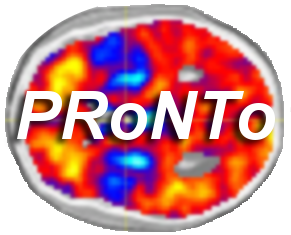
\includegraphics[width=10cm]{images/pronto_logo.png}
%\end{center}

\vspace*{\stretch{1}}
\noindent\hspace*{\centeroffset}\makebox[0pt][l]{\begin{minipage}{\textwidth}
\flushright
\textbf{\Huge{\HPRoNTo Manual}}
{\noindent\rule[-1ex]{\textwidth}{5pt}\\[2.5ex]}
\hfill{{\huge The \hPRoNTo Development Group} \\
\Large{(and honorary members)}\\}
\vspace{20mm}
\hfill{
John Ashburner \\
Carlton Chu\\
Andre Marquand\\
Janaina Mourao-Miranda\\
Joao M. Monteiro\\
Christophe Phillips\\
Jonas Richiardi\\
Jane Rondina\\
Maria J. Rosa\\
Jessica Schrouff}
\end{minipage}}

\vspace{\stretch{2}}
\noindent\hspace*{\centeroffset}\makebox[0pt][l]{\begin{minipage}{\textwidth}
\flushright
{\footnotesize
Machine Learning \& Neuroimaging Laboratory\\
Centre for Computational Statistics and Machine Learning\\
Computer Science department, UCL\\
Malet Place, London WC1E 6BT, UK \\
\today\\
\url{http://www.mlnl.cs.ucl.ac.uk/pronto}}
\end{minipage}}

%-----------------------------------------------------------------------

\dominitoc 
\tableofcontents
\newpage

%%%%%% INTRODUCTION %%%%%%
%==========================================
% $Id$

\chapter{Introduction}
\label{chap:intro}
\minitoc

%==========================
\section{Background}
%==========================

Advances in neuroimaging techniques have radically changed the way neuroscientists address questions about functional anatomy, especially in relation to behavioural and clinical disorders. Many questions about brain function, previously investigated using intracranial electrophysiological recordings in animals can now be addressed non-invasively in humans. Such studies have yielded important results in cognitive neuroscience and neuropsychology. Amongst the various neuroimaging modalities available, Magnetic Resonance Imaging (MRI) has become widely used due to its relatively high spatial and temporal resolution, and because it is safe and non-invasive. By selecting specific MRI sequence parameters, different MR signals can be obtained from different tissue types, giving images with high contrast among organs, between normal and abnormal tissues and/or between activated and deactivated brain areas. MRI is often sub-categorized into structural MRI (MRI) and functional MRI (fMRI). Examples of other of imaging modalities that measure  brain signals are Positron Emission Tomography (PET), ElectroEncephaloGraphy (EEG) recordings and MagnetoEncephaloGraphy (MEG) recordings. Neuroimaging data are inherently multivariate, since each measure (scan or recording) contains information from thousands of locations (e.g. voxels in MRI or electrodes in EEG). Considering that most brain functions are distributed processes involving a network of brain regions, it would seem desirable to use the spatially distributed information contained in the data to give a better understanding of brain functions in normal and abnormal conditions. 

The typical analysis pipeline in neuroimaging is strongly rooted in a mass-univariate statistical approach, which assumes that activity in one brain region occurs independently from activity in other regions. Although this has yielded great insights over the years, specially in terms of function localization, and continues to be the tool of choice for data analysis, there is a growing recognition that the spatial dependencies among signal from different brain regions should be properly modelled. The effect of interest can be subtle and spatially distributed over the brain - a case of high-dimensional, multivariate data modelling for which conventional tools may lack sensitivity. 

Therefore, there has been an increasing interest in investigating this spatially distributed information using multivariate pattern recognition approaches, often referred to as  multi-voxel pattern analysis (MVPA) (see  \cite{Norman2006},  \cite{Haynes2006} and \cite{Pereira2009}). Where pattern recognition has been used in neuroimaging, it has led to fundamental advances in the understanding of how the brain represents information and has been applied to many diagnostic applications. For the latter, this approach can be used to predict the status of the patient scanned (healthy vs. diseased or disease A vs. B) and can provide the discriminating pattern leading to this classification. Pattern recognition techniques can also be used to identify relationships between patterns of brain structure or activity and continuous measures such as age or a clinical score. Such information can then be used to predict individual-level measures for new individuals (i.e. regression models).

Several active areas of research in machine learning are crucially important for the difficult problem of neuroimaging data analysis: modelling of high-dimensional multivariate time series, sparsity, regularisation, dimensionality reduction, causal modelling, and ensembling to name a few. However, the application of pattern recognition approaches to the analysis of neuroimaging data is limited mainly by the lack of user-friendly and comprehensive tools available to the fundamental, cognitive, and clinical neuroscience communities. Furthermore, it is not uncommon for these methods to be used incorrectly, with the most typical case being improper separation of training and testing datasets.


%==========================
\section{Methods}
%==========================

PRoNTo (Pattern Recognition for Neuroimaging Toolbox) is a toolbox based on pattern recognition techniques for the analysis of neuroimaging data. Statistical pattern recognition is a field within the area of machine learning which is concerned with automatic discovery of regularities in data through the use of computer algorithms, and with the use of these regularities to take actions such as classifying the data into different categories \cite{Bishop2006}. In PRoNTo, brain images are treated as spatial patterns and statistical learning models are used to identify statistical properties of the data that can be used to discriminate between experimental conditions or groups of subjects (classification models) or to predict a continuous measure (regression models).


PRoNTo is \matlab based and includes five main modules: `Data \& Design', `Prepare feature set', `Specify model', `Run model' and `Compute weights'. The results can displayed in terms of the performance of the estimated model, as well as in terms of model parameters. Additional review options enable the user to review information about the data, features and models. All modules were implemented using a graphical user interface (GUI) and the MATLAB Batch System. Using the MATLAB Batch System the user can run each module as batch jobs, which enables a very efficient analysis framework.  All information about the data, experimental design, models and results are saved in a structure called PRT. PRoNTo also creates additional files during the analysis that are described in details in the next chapters.

The toolbox code will be distributed for free, but as copyright software under the terms of the GNU General Public License as published by the Free Software Foundation. 

\subsection{Inputs and preprocessing}

In terms of neuroimaging modalities, PRoNTo accepts NIFTI files. Mostly designed to analyse structural and functional Magnetic Resonance Imaging and PET, it can be used on any dataset converted to a NIFTI file. It assumes that the neuroimaging data has been previously pre-processed using SPM (\url{http://www.fil.ion.ucl.ac.uk/spm/}) or a similar software for neuroimaging analysis. In general, raw fMRI data should be previously corrected for movement artefact (realigned) and time difference in slice acquisition (slice time correction), mapped to a common template (normalized) and spatially smoothed. The normalisation and spatial smoothing steps might not be necessary for single subject analysis.  

In addition the General Linear Model (GLM) can be applied as a pre-processing step for pattern recognition analysis. In this case, the GLM coefficients (e.g. beta images in SPM) will correspond to the spatial patterns. Using beta images should be preferred in the case of event-related designs with short inter-stimulus time and/or event duration to better take into account the Haemodynamic Response Function (HRF). \textbf{Important note}: Beta images output by SPM contain NaNs (Not a Number) values in some voxels. For better performance of the model, a mask should be created to exclude the corresponding voxels from the analysis. Practically, a mask should be built (e.g. using SPM imcalc batch or a script provided in `utils') to specify which voxels have scalar values (1 in mask) or NaN or 0 value (0 in mask). The updated mask should then be input in the Data \& Design window. To ease this extra preprocessing step, a script is provided in \textit{your PRoNTo folder/utils}. It takes as inputs the images (i.e. beta images in nifti format), the mask to update (e.g. SPMnoeyes.nii provided in \textit{your PRoNTo folder/mask}) and the directory to save the updated mask. Inputs are optional, and just typing in the \matlab command: prt\_utils\_update\_mask will ask for the different inputs using file and path selectors.

Raw structural MRI data should be previously mapped to a common template (normalized) and spatially smoothed. Raw PET data should be realigned, normalized and smoothed. PET data is also usually scaled. This operation can be performed before hand or during the building of the feature set.

%In the current version of the software, regression models and regressing out effect of covariates from the data is provided only when selecting images by scans (i.e. for one image per subject). Therefore, we suggest that users interested in removing covariates from datasets with a (fMRI) design perform a GLM analysis before hand and input the derived beta images as patterns.

\subsection{Machine learning algorithms}

In PRoNTo different pattern recognition algorithms correspond to different machines. The machine library in PRoNTo v2 includes four classification models: Support Vector Machine (\cite{Cristianini2000}, \cite{Mourao-Miranda2007}), Gaussian Process Classifier (binary and multiclass, \cite{Rasmussen2006}, \cite{Marquand2010}) and L1-Multiple Kernel Learning \cite{Rakotomamonjy2008}. Four regression models are available: Kernel Ridge Regression \cite{ShaweTaylor2004}, Relevance Vector Regression \cite{Tipping2001}, Gaussian Process Regression \cite{Rasmussen2006} and L1-Multiple Kernel regression \cite{Rakotomamonjy2008}. New machines will be added to the library in future versions of the toolbox. %, Random Forest \cite{Geurts2006}

PRoNTo should facilitate the interaction between machine learning and neuroimaging communities. On one hand the machine learning community should be able to contribute to the toolbox with novel published machine learning models. On the other hand the toolbox should provide a variety of tools for the neuroscience and clinical neuroscience communities, enabling them to ask new questions that cannot be easily investigated using existing statistical analysis tools. 


%=====================
\section{Installing \& launching the toolbox}
%=====================
\label{sec:Installation}

In order to work properly, PRoNTo requires 2 other softwares:
\bi
\item a recent version of \matlab. We used versions 7.10 (R2010a) to 8.4 (R2014b) to develop PRoNTo, and it will not work with earlier versions\footnote{Any later \matlab~version should work, {\it in theory}.}. 
\item SPM8\cite{SPM8} installed on your computer\footnote{SPM8 can be dowloaded from the following website: \url{http://www.fil.ion.ucl.ac.uk/spm/software/}. You should install it in a suitable directory, for example {\tt C:\bslash SPM8\bslash }, then make sure that this directory is on the \matlab path. No need to include the subdirectories!}. SPM12b and SPM12 are also supported.
\ei

PRoNTo latest public version can be downloaded, after registration, from the following address: \url{http://www.mlnl.cs.ucl.ac.uk/pronto/prtsoftware.html}.

\textbf{Important note}: if you already have a version of SPM on your computer, please download the latest updates from the website. Various bugs, especially in terms of weight visualization, arise from out of date SPM versions.

\subsection{Installation}
%--------------------------------------

After downloading the zipped file containing PRoNTo, the installation proceeds as follow:
\begin{enumerate}\addtolength{\itemsep}{-1\baselineskip}
\item	Uncompress the zipped file in your favourite directory, for example {\tt C:\bslash PRoNTo\bslash };\\
\item	Launch \matlab ;\\
\item	Go to the ``{\tt File}'' menu $\rightarrow$ ``{\tt Set path}'';\\
\item	Click on the ``{\tt Add folder}'' button and select the PRoNTo folder, i.e. {\tt C:\bslash PRoNTo\bslash } if you followed the example;\\
\item	Click on save.
\end{enumerate}

Some routines, in particular the 'machines', are written in C++ ({\tt .cpp} files) for increased efficiency. We are trying to provide these compiled routines for the usual Operating Systems (OS's) such as: Windows XP (32 bits), Windows 7 (64 bits), Mac OS 10, Linux (32 and 64 bits). If your OS is not listed or routines do not work properly then you should compile the routines for your specific OS\footnote{you can also contact us and we'll try to come up with a solution for your system.}. 

\subsection{Launching and batching}
%--------------------------------------

Once installed, there are three ways to call up PRoNTo functionalities.
To launch the toolbox GUI, just type {\tt prt} or {\tt pronto} at the \matlab \ prompt and the main GUI figure will pop up, see Fig.~\ref{fig:mainGUI}. From there on simply click on the processing step needed (see Part \ref{sec:GUI} of this manual). Most functions of PRoNTo have been integrated into the {\tt matlabbatch} batching system \cite{matlabbatch} (like SPM8) and the batching GUI is launched from the main GUI by clicking on the {\tt Batch} button  (see Part \ref{sec:BATCH} of this manual).
Of course most tools can also be called individually by calling them directly from the \matlab \ prompt, or for scripting in a {\tt .m} file  (see Part \ref{sec:ADVTOP} of this manual).

\begin{figure}[!htbp]
  \begin{center}
      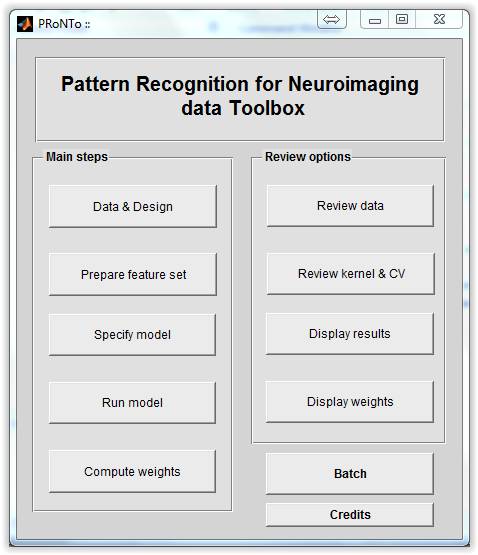
\includegraphics[height=7cm]{images/fig2_main_prt.png}
   \caption{Main GUI interface: each button launches a specific processing step.}
    \label{fig:mainGUI}
  \end{center}
\end{figure}	

\subsection{Troubleshooting}
%--------------------------------------
\subsubsection{Compiling libsvm}
Some problems when using SVMs might arise due to  libsvm, in which case, you might need to compile it on your own. The first thing that needs to be done is to download the desired libsvm version (usually the latest one) from the following website: \url{http://www.csie.ntu.edu.tw/~cjlin/libsvm/}. Then, the process will depend on your operating system.

If the steps described bellow do not work, please refer to the {\tt README} file that comes with libsvm.

\paragraph{Microsoft Windows}
\begin{itemize}
    \item Make sure you have a C++ compiler install. If not, you can install Microsoft Visual C/C++;
    \item Copy the libsvm folder to the `machines' directory of your PRoNTo instalation\\(e.g. C:\bslash PRoNTo\bslash machines\bslash);
    \item Open a DOS command window and change to the libsvm folder in the previous step ({\tt cd C:\bslash PRoNTo\bslash machines\bslash libsvm-3.17\bslash}). If the environment variables of VC++ have not been set, run the following command:\\{\tt C:\bslash Program Files\bslash Microsoft Visual Studio 10.0\bslash VC\bslash bin\bslash vcvars32.bat}. This command might be different, depending on the path of your Visual Studio installation;
    \item In the libsvm folder run the command: {\tt nmake -f Makefile.win clean all} 
    \item If no errors appear, open MATLAB;
    \item Change to the `matlab' folder inside the libsvm folder (e.g. C:\bslash PRoNTo\bslash machines\bslash libsvm-3.17 \bslash matlab\bslash);
    \item Run {\tt make} in the MATLAB Command Window. If there are no errors, you have just successfully compiled libsvm to be used with MATLAB.
\end{itemize}

Remember, if you want to use the version that you have just compiled, you have to add the libsvm folder to your path in MATLAB. If you have more than one libsvm folder inside the `machines' folder, please remove one of them from the MATLAB path. You should only have one libsvm folder in your path.


\paragraph{Unix (Mac OS or Linux)}

\begin{itemize}
    \item Make sure you have a C++ compiler installed. If you are using Mac OS, please install `Xcode'. On Linux systems, you should already have `gcc' installed;
    \item Copy the libsvm folder to the `machines' directory of your PRoNTo instalation\\(e.g. {\tt /home/<username>/PRoNTo/machines/});
    \item Open a terminal window and change to the `machines' directory: {\tt cd PRoNTo/machines/}
    \item Compile libsvm by running the following command: {\tt make}
    \item If no errors appear, open MATLAB;
    \item Change to the `matlab' folder inside the libsvm folder (e.g. PRoNTo/machines/libsvm-3.17/matlab/);
    \item Run {\tt make} in the MATLAB Command Window. If there are no errors, you have just successfully compiled libsvm to be used with MATLAB.
\end{itemize}

Remember, if you want to use the version that you have just compiled, you have to add the libsvm folder to your path in MATLAB. If you have more than one libsvm folder inside the `machines' folder, please remove one of them from the MATLAB path. You should only have one libsvm folder in your path.

%==========================
\section{What's new?}
%==========================

\subsection{Version 2.0}
This version of the toolbox (2015) aims at providing multiple new functionalities, including:
\begin{itemize}
\item \textbf{Build one kernel per modality}: When there are multiple modalities in the same dataset, it is now possible to build one kernel per modality and use them in the same model later on. If this option is not chosen, the selected modalities can still be concatenated as additional samples/examples or sessions (if they have the same dimensions) or used separately.
\item \textbf{Build one kernel per region}: It is also possible to specify an atlas, comprising regions of interest (ROIs) as defined by values in the atlas ranging from 1 to \textit{number of ROIs}. For each anatomically defined ROI, a kernel will be built taking into account the multivariate pattern within the region. It is possible to use this feature in combination with the previous one (e.g. one kernel per region and per modality, or concatenate modalities as additional samples and build one kernel per region).
\item \textbf{New machines}: The list of available machines was extended, and now includes L1-Multiple Kernel Learning (MKL, classification and regression). The latter corresponds to a hierarchical model defined by weights at two levels: the voxel level and the kernel level (i.e. ROI and/or modality).
\item \textbf{Flexible cross-validation}: A GUI is provided to manually specify a custom cross-validation matrix. It allows to either specify a basis (e.g. leave-one-subject-out), load a .mat or specify the number of folds. Then the user can, for each fold, select which examples are part of the training set, test set, or won't be used. The resulting matrix can be saved for further use.
\item \textbf{Nested cross-validation for hyperparameter optimization}: It is now possible to optimize the hyperparameter(s) of some machines (e.g. the soft-margin parameter, C, in SVM) using a nested cross-validation (CV) framework. The number of folds in the nested cross-validation, used only to estimate the value of the hyperparameter leading to the highest performance, does not need to be the same as the `outer' cross-validation (i.e. the one estimating the final model performance). For example, to decrease computational expenses, the nested CV can be a 4-fold CV while the outer CV can be a leave-one-out.
\item \textbf{Display results}: The display of the results was divided into two modules (Display Results and Display Weights). This allows to review the model performance in one window, with all the statistics. A new graph displaying the effect of the hyperparameter (if optimized) was also included.
\item \textbf{Weights per ROI}: For each model it is possible to build images representing the weights per voxel and also images summarising the weights per regions of interest as defined by an atlas. If an MKL model was built on ROIs, the contribution of each ROI (regional weight) is explicitly derived. On the other hand, if a simple kernel model was selected (e.g. SVM on the whole brain), the weights per voxel will be averaged (in absolute value) within each region, as defined by an atlas specified by the user. In both cases, an additional image, with weights per ROI, is created and saved.
\item \textbf{Display weights}: The weights of each model can be displayed at the voxel level in this window. If weights per ROI were derived (either summarized or from an MKL on ROIs), weights per region can be displayed as an image, as well as in a sorted list of regions. The same applies for MKL models on multiple modalities. A histogram is also displayed representing the contribution/weight of each ROI/modality to the model. The table can be exported as text for future use in publications/communications.
\end{itemize}

\subsection{Version 1.1}
In 2012, PRoNTo v1.1 was released mainly to provide bug fixes for version v1.0. Two features were also added:
\begin{itemize}
\item automatic compiling of the machines (in particular: no more issues with SVM, nor with Matlab toolboxes and paths).
\item k-folds Cross-Validation (CV): specify the number of folds or set it to 1 for half-half CV (train on first half, test on second).
\end{itemize}

\subsection{Version 1.0}
Launched in 2011, this version of PRoNTo allows to perform all the analysis steps, from Data \& Design to computing the weights for three classification machines (SVM, binary and multi-class GP) and two regression machines (KRR, SVR).

\subsection{How to cite}
%--------------------------------------
Please cite \cite{Schrouff2013} when using PRoNTo analyses in any type of publication. In addition, Multiple Kernel Learning analyses should refer to a second paper (submitted, tba)\footnote{When the paper gets accepted, this section will be updated and the paper will be listed in the documentation section of the website}. Meanwhile, please cite \cite{Schrouff2014} for MKL analyses and \cite{Schrouff2013a} for a posteriori weight summarization using atlas-defined regions of interest. 

%==========================
\section{Main contributors}
%==========================
PRoNTo is  developed by the Machine Learning \& Neuroimaging Laboratory, Computer Science department, University College London, UK (\url{ http://www.mlnl.cs.ucl.ac.uk}) and associated researchers.

The main contributors, in alphabetical order, are: 
\begin{description}
	\item[Dr. John Ashburner] is a Professor of Imaging Science at the Wellcome Trust Centre for Neuroimaging at the University College London Institute of Neurology. He is mainly interested in modelling brain anatomy from MR scans, and more recently in applying pattern recognition methods to make predictions about individual subjects. He is a co-developer of the SPM software (intra- and inter-subject registration, tissue classification, visualization and image file formats), which is used internationally by thousands of neuroimaging researchers. He has a Web of Science h-index of 63.  He did not contribute any actual code to PRoNTo, but he did attend many of the meetings;
    \item[Dr. Carlton Chu] is a research scientist at  Google DeepMind. Before joining DeepMind, he was a research fellow in brain imaging at the National Institute of Mental Health (NIMH), NIH. He received the B.Eng. degree (1\textsuperscript{st} class Honours) from Auckland University, in 2002 and the master of Biomedical Engineering from University of New South Wales, in 2004. Carlton obtained a PhD in Neuroimaging method from University College London in 2009, working in the statistical methods group at the Wellcome Trust Centre for Neuroimaging, creators of the famous ``SPM'' program. There he developed innovative pattern recognition methods to automatically detect the early stages of neurodegenerative diseases such as Alzheimer's and Huntingdon's from structural brain images. In 2007, Carlton won the first prize in the 2nd Pittsburgh Brain Activity Interpretation Competition (PBAIC), a prestigious international competition involving the application of machine learning to the problem of classification of brain activity. He led a small research team to victory, acclaim from peers in the field, and the \$10K first prize. His current research interests include image segmentation using convolutional neural networks and applications of deep-learning. Carlton was involved in the development of PRoNTo version 1.0;
	\item[Dr. Andre Marquand] is an Junior Principal Investigator at the Donders Institute for Brain Cognition and Behaviour and a Lecturer at the Institute of Psychiatry, Psychology and Neuroscience, King's College London.  His research focuses on the application of probabilistic machine learning techniques to neuroimaging data, particularly for clinical applications. His recent work includes the development of multi-class, multi-task and multi-modality pattern classification methods that offer many advantages over current techniques including more sensitive and specific detection of disease effects;
	\item[Dr. Janaina Mourao-Miranda] is a Wellcome Trust Senior Research Fellow at the Centre for Computational Statistics and Machine Learning (CSML), UCL.  Over the past years her research has involved developing and applying pattern recognition methods to analyze neuroimaging data, in particular brain activation and structural patterns that distinguish between controls and patients. Her current research focuses on developing machine-learning models to investigate complex relationships between neuroimaging data and multidimensional descriptions of mental health disorders. She has been coordinating the PRoNTo developments and contributed to PRoNTo versions 1.0, 1.1 and 2.0;
	\item[Mr. Joao M. Monteiro] is a MPhil/PhD Student at University College London under the supervision of Prof. John Shawe-Taylor and Dr. Janaina Mourao-Miranda. His research focuses on the application of unsupervised machine learning methods to neuroimaging. He contributed to PRoNTo versions 1.1 and 2.0;
	\item[Dr. Christophe Phillips] is FRS-FNRS Research Associate at the Cyclotron Research Centre and adjunct Assistant Professor at the Department of Electrical Engineering and Computer Science, University of Li\`ege, Belgium. His research focuses on the processing of multi-modal neuroimaging data. Recent work within the field of ``brain decoding'' aimed at distinguishing between levels of consciousness in unresponsive patients or between typical and atypical Parkinson Disease patients using Positron Emission Tomography (PET) imaging, as well as tracking mnesic traces in trained healthy subjects with fMRI;
	\item[Dr. Jonas Richiardi] is a Marie Curie researcher at the University of Geneva (Department of Fundamental Neuroscience). His research interests include the combination of imaging modalities with other biological information sources including genomic data, learning with graphs, machine learning for neuroimaging, brain connectivity / resting-state data analysis, interpretability of brain decoding results, and functional biomarkers. He has been involved with the organization of the workshop on Pattern Recognition in NeuroImaging since the beginning;
	\item[Dr. Jane Rondina] is a research fellow at the University College London Institute of Neurology. Previously, she was a post-doctoral research associate at the Centre for Neuroimaging Sciences, King's College London. In the past years, her research has involved application of pattern recognition methods to neuroimaging data and development of a stability-based method for feature selection and mapping in neuroimaging. Her current research focuses on prognosis and prediction of treatment response, mainly addressing approaches to combine complementary information from different imaging modalities and other sources of data (clinical, demographic and genetic). She contributed to the development of PRoNTo version 1.0. She is also involved in incorporation of new resources for version 3.0;
	\item[Dr. Maria J. Rosa] is an imaging scientist at IXICO, plc. Before, she was a Post-Doctoral Research Fellow at the Institute of Psychiatry, King's College London (KCL) and a Wellcome Trust post doctoral research associate at the Centre for Computational Statistics and Machine Learning (CSML), UCL. Maria's main area of work is the development and application of machine learning and multivariate methods to neuroimaging data. She did her PhD at the Wellcome Trust Centre for Neuroimaging, UCL. She contributed to PRoNTo versions 1.0, 1.1 and 2.0;
	\item[Dr. Jessica Schrouff] got her PhD from the University of Li\`ege, under the supervision of Dr. C. Phillips. She is a post-doctoral researcher at the Laboratory of Behavioral and Cognitive Neuroscience, Stanford University. Her research focuses on the detection and characterization of memory traces in resting state wakefulness using machine learning techniques, based on fMRI data (Ph.D. thesis) and intracranial EEG recordings. She contributed to PRoNTo versions 1.0, 1.1 and 2.0. She has also started adapting the toolbox for analysis of electrophysiological recordings (version 3.0);
\end{description}

We also thank students and post-docs for their help in testing the software and writing this manual: Dr. Liana Lima Portugal, Liane Canas, Dr. Ana Regia Neves, Rochelle Silva, Dr. Orlando Fernandes Junior and Dr. Qinquan Gao. 

%==========================
\section{Acknoweldgements}
%==========================
PRoNTo is the deliverable of a Pascal Harvest project coordinated by Dr. J. Mourao-Miranda and its development was possible with the financial and logistic support of 
\begin{itemize}
\item the Department of Computer Science, University College London  (\url{http://www.cs.ucl.ac.uk});
\item the Wellcome Trust (\url{http://www.wellcome.ac.uk/}) under grants no. WT086565/Z/08/Z and no. WT102845/Z/13/Z;
\item PASCAL2 (\url{http://www.pascal-network.org}) and its HARVEST programme;
\item the Fonds de la Recherche Scientifique-FNRS (\url{http://www.fnrs.be}), Belgium;
\item Funda\c{c}\~{a}o para a Ci\^{e}ncia e Tecnologia - FCT (\url{http://www.fct.pt}), Portugal;
\item Swiss National Science Foundation (PP00P2-123438) and Center for   Biomedical Imaging (CIBM) of the EPFL and Universities and Hospitals  of Lausanne and Geneva.
\item The EU Marie Curie Action under grant FP7-PEOPLE-2011-IOF \# 299500.
\item The Laboratory of Behavioral and Cognitive Neuroscience, Stanford University.
\end{itemize}

%PRoNTo is written for MATLAB X.Y (R20ZZb) and onwards. Some routine may need to be compiled for your specific OS.


%%%%%% GUI HELP %%%%%%
%==========================================
\part{Description of PRoNTo tools}
\label{sec:GUI}
% Description of each main and review step
% $Id: gui_data.tex 395 2011-11-17 22:34:59Z cphillip $
%
% Written by Maria Joao Rosa
%_______________________________________________

\chapter{Data \& Design}
\label{chap:DataDesign}
\minitoc

\section{Introduction}

The first step in a statistical analysis of neuroimaging data,  whether it's in a pattern recognition or general linear model (GLM) framework, usually entails providing to the analysis software all the information regarding the data and experimental design. PRoNTo is no exception. After preprocessing the data (if required), the analysis in PRoNTo starts with the `Data and Design' module. It is important to note that PRoNTo does not perform any spatial or temporal pre-processing, and if not performed with another software, pattern recognition might be affected by misalignment and noise in the data. 

In the `Data and design' module the user can enter the image/scan files, experimental conditions (TR, durations and onsets of events), as well as other parameters, covariates and regression values. PRoNTo supports multi-modality datasets and therefore it allows the user to enter more than one data modality, such fMRI, MRI, PET and ASL, per analysis. This module is therefore essential for the rest of the framework and stores all the information that is needed from the data to be used by the rest of the software modules, such as feature set preparation, model specification and estimation. 

Below is a summary of what the `Data and Design' module does. The Methods section discusses how the module is organised and what its main output is. It also mentions a few issues that need to be taken into consideration when entering the information and how they affect subsequent steps. This chapter then presents the graphical user interface (GUI) that is used to enter the data and design information and how it is used. Finally, the chapter finishes by mentioning the corresponding `Data and Design' {\tt matlabbatch} module, and particular issues that do not apply to the GUI.

\section{Methods}

\subsection{Data and design input}

PRoNTo provides two types of interfaces for entering the data and design information, a PRoNTo-specific graphical user interface (GUI) and the  {\tt matlabbatch} system that is also currently used by SPM. These two interfaces are also available for the other modules, as discussed in the Introduction chapter.

The information that needs to be entered is almost exactly the same for both the GUI and batch (the small differences are explained below in the  {\tt matlabbatch} section) and, more importantly, the output is exactly the same. Therefore it is up to the user to decide which system is best suited for his/her analyses. For instance, the GUI can be used as a first approach to the toolbox and by users not familiar with SPM, whilst the batch can be used by more advanced or SPM users, who know how to take advantage of the batch system to optimise their analyses.

As mentioned, PRoNTo supports multi-modality analyses. Therefore the data and design module is prepared to receive as input the following types of data: fMRI, sMRI, PET and beta images (created from a previous GLM analysis). Other types of data can also be entered at the user's risk, as long as they comprise nifti files.

Regardless of which interface the user chooses to enter the data and design (GUI or batch), the organisation is very similar and starts (after choosing the directory to save {\tt PRT.mat}) with the definition of Groups. In neuroimaging datasets, it is common to have a few subjects with a lot of images/scans per subject, such as the time-series in fMRI. However, the opposite is also common: lots of subjects with one image per subject, such as encountered in PET or MRI studies. Therefore, for each group, PRoNTo provides two ways of entering the rest of the information, i.e. subjects, modalities and design, which are referred to as the `select by subject' or `select by scans' option, respectively (as is shown below). If one chooses to enter the data by `scans', PRoNTo allows the user to enter, for each modality, all subjects (one image/scan per subject) at once, which is a lot quicker than entering each subject at a time. It is important to note that when using \textit{Regression} models this is the only way of inputing the data. As explained below, only the `select by scans' option allows the users to enter regression values (one value per subject/image). This option however is not appropriate for modalities which have an experimental design and more than one image per subject, such as fMRI. For these datasets the user should choose the `subjects' option. For each subject one can specify the modalities, experimental conditions and enter more than one image/scan. Both options are valid and produce exactly the same output structure (if used with the same dataset). 

\subsection{Data and design output}

The output of the `Data and Design' module is the PRT structure (as discussed in the Introduction). This structure contains subfields with all the information that is needed from the data for the subsequent analysis steps and it is saved in a `PRT.mat' file. For advanced users the fields of this structure can be edited directly and saved, therefore bypassing the need to use the GUI or  {\tt matlabbatch} to create the PRT. However, this structure is the core of PRoNTo and should be carefully created because it affects everything else.

\subsection{Review}

The `Data and Design' module also allows the user to review the information that has been entered (through the GUI, batch or manually). The main aim of the `Review' function is to check if the data and design has been correctly specified. It can also be used to inspect if the design is appropriate for subsequent analysis. For example, the review window shows the number of subjects in each group, and for modalities with experimental design, it can be used to show and alter the number of used and unused scans (see below). 

\subsection{HRF correction}

For datasets such as fMRI, there is a very important issue that needs to be carefully addressed when specifying the data and design. As is well known, the hemodynamic response function (HRF) is a delayed and dispersed version of the underlying neuronal response to an experimental event (Figure \ref{Fig2.1}). This means that, depending on the TR, the effect of the HRF can be felt over multiple scans, and therefore the acquired scans are not independent and might contain information from both past and present events. This can confound subsequent analyses and needs to be accounted for. For instance, in SPM, the stimulus time-series are convolved with a canonical HRF. Although convenient in the GLM framework, the convolution approach is not appropriate in the pattern recognition context. Therefore, the solution used in PRoNTo is to discard all overlapping scans. This is done as follows: PRoNTo allows the user to control a delay (time it takes for the hemodynamic response to peak after the stimulus) and overlap (width of the response) parameter that determine the shape of the HRF. As can be seen in Figure \ref{Fig2.1}, the delay means that the scans corresponding to a given condition are actually shifted in time, and the overlap means that the number of independent scans, for which the signal corresponds only to a given condition, is smaller than the total number of acquired scans for each condition. Given the delay, PRoNTo finds which scans correspond to each condition and discards the last scans in the time-series for which the response has not yet peaked. It then uses the overlap to determine which consecutive scans contain information from only one condition (i.e. the response does not overlap with the response from the previous condition) and discards the ones for which there is overlap (as shown in Figure \ref{Fig2.1}, bottom right). The discarded scans are not actually deleted but are not used in further analyses.

When using the GUI, the default value for the HRF parameters is 0 seconds and can only be changed in the `Review' window (as shown below). Therefore, for fMRI, the user should review the data and design and change these parameters to a more appropriate value (e.g. 6 seconds each). In the {\tt matlabbatch}, the default value for these parameters is also 0 seconds but can be changed directly within the batch (no need to open Review window). Again, for fMRI, these values should be changed (e.g. to 6 seconds).

Importantly, if one wants to avoid discarding scans and having to correct for the shape of the HRF, as explained in the above paragraph, one should use as input the beta (coefficients) images obtained by first running a GLM analysis on the original data. The GLM analysis accounts for the HRF delay and overlap using the convolution approach. This is normally the best approach in case of rapid event-related design experiments, in which there can be a lot of overlap, i.e. the number of discarded scans can be very high.

\begin{figure}[!h]
  \begin{center}
      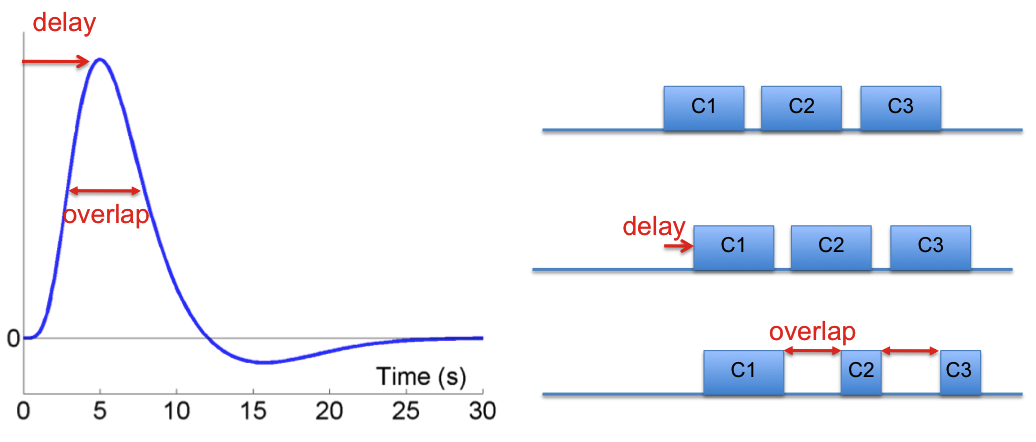
\includegraphics[height=2.2in]{images/Figure1.png}
   \caption{HRF correction. On the left is the standard HRF response. On the right is the effect of the delay and overlap on the number of independent scans (C1, C2 and C3 correspond to three different experimental conditions and the blue boxes correspond to various scans acquired during each condition). In fMRI datasets, the nature of the HRF (i.e. being a delayed and dispersed version of the neuronal response to an experimental event) might lead to less independent scans/events than the ones originally acquired. In PRoNTo, this issue is accounted for by discarding overlapping scans.}
    \label{Fig2.1}
  \end{center}
\end{figure}

The steps to specify the information relative to the data and design using both the GUI and the {\tt matlabbatch} system are described in the following sections.

\section{Graphical User interface}

The graphical user interface to specify the data and design is presented in Figure \ref{Fig2.2}. This GUI can be launched by typing `prt' in the Matlab window and then clicking the first button on the left, in the main steps panel.

\begin{figure}[!h]
  \begin{center}
      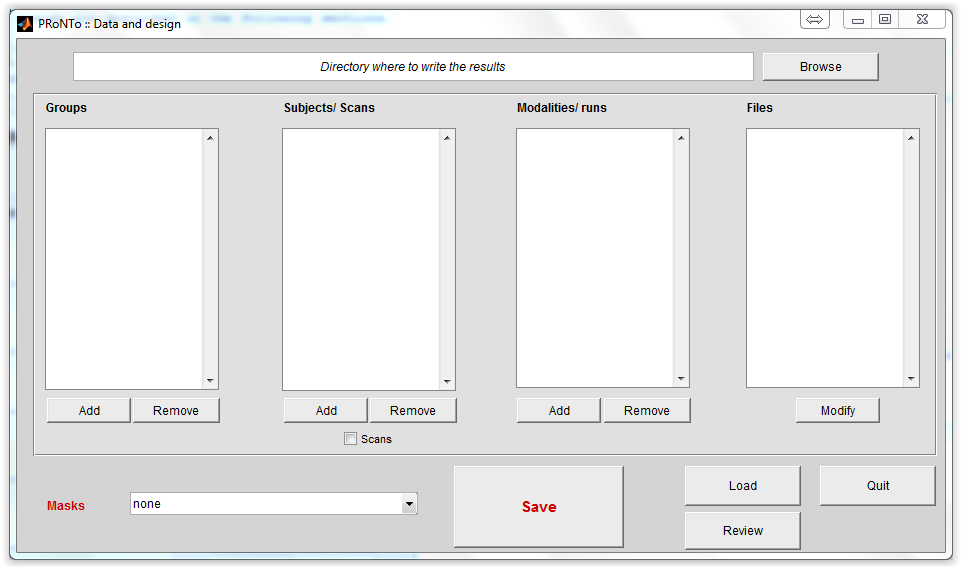
\includegraphics[height=2.7in]{images/Figure2.png}
   \caption{Data and design graphical user interface. This interface allows the user to enter all the information relative to the data, including the experimental design and masks. After introducing all the fields, PRoNTo creates the PRT structure, which is saved in the specified directory, as `PRT.mat' file.}
    \label{Fig2.2}
  \end{center}
\end{figure}

\subsection{PRT directory}

The first thing the user should specify is the directory in which to save the PRT structure. This can be done by browsing existing directories (previously created by the user) from the top of the data and design interface (Figure \ref{Fig2.2}). It is recommended to have different directories for different datasets (note that a dataset can include different modalities in case of multimodal analysis) because PRoNTo overwrites an existing PRT in the selected directory. The later modules in PRoNTo will then add more fields to this structure with further information, such as the models, features and kernels used in subsequent analyses. The file created is called `PRT.mat'.

\subsection{Groups}

The group panel allows one to add or remove a group of subjects. The minimum number of groups is one, but there is no maximum number. When `Add' is clicked, the user should provide a name to the group. Any alphanumeric string is sufficient and there should be no spaces in the string (this applies to all names throughout the toolbox). The name of the group can be later modified by right clicking on the name. When `Remove' is clicked, all the information relative to this group (including all subjects and corresponding data) is deleted. PRoNTo does not restore the deleted information and it can only be re-entered again by clicking `Add'.

The following panel after `Groups' is `Subjects/Scans'. Here, as mentioned above, there are two ways of entering the data: by `subjects' or by `scans'. The former is chosen by clicking `Add' under the `Subjects/Scans' panel and filling in the fields for each added subject at a time. The latter is done by clicking the tick box `Scans' under the `Subjects/Scans' panel. The subjects panel is then de-activated and the user can enter the modalities and files straight away. The fields to be filled under these two options are described below.

\subsection{Subjects}

\paragraph{Select by scans} The `select by scans' option allows the users to skip the subject step. To identify that this option has been selected, PRoNTo writes `scans' in the subjects panel (Figure \ref{Fig2.3}). The user can then add modalities and for each modality a new window will appear (bottom of Figure \ref{Fig2.3}). 

%It is important to remember that when the `scans' box is clicked all the information in the subjects panel is automatically deleted! 
% NOTE:AR-edit, no need for so many exclamations
It is important to remember that when the `scans' box is clicked all the information in the subjects panel is
automatically deleted. 
Unselecting the `scans' box also deletes all the information!

\paragraph{Select by subjects} The `Subjects/Scans' panel allows the user to add/remove subjects. This panel works exactly like the groups panel, but the subject name is automatically generated. This name can be later modified by right clicking on it. For each subject one can then specify the modalities in the next panel.

\begin{figure}[!h]
  \begin{center}
      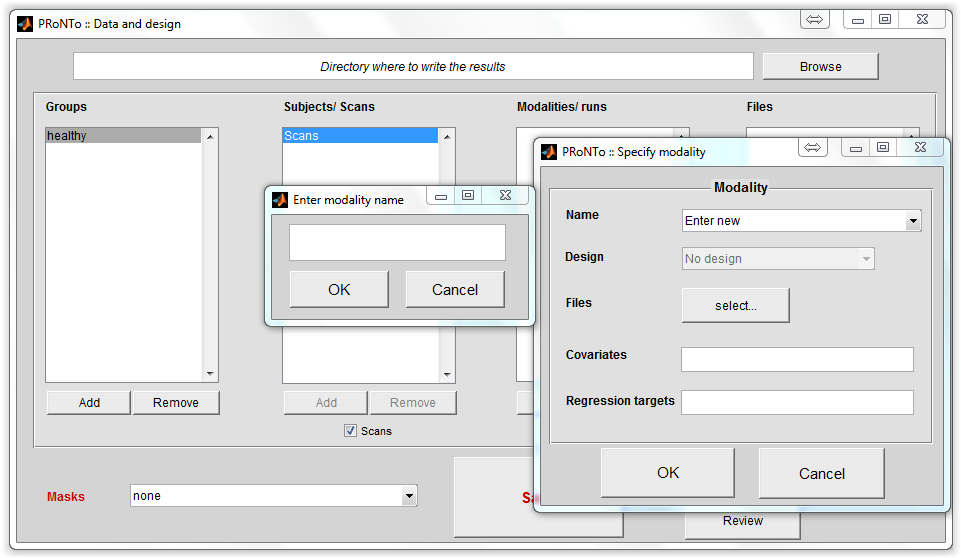
\includegraphics[height=3.5in]{images/Figure3.png}
   \caption{Data and design graphical user interface. If one chooses to specify everything using the `Scans' option (tick box below the `Subjects/Scans' panel), one can introduce the data for all subjects at once for each modality, but one cannot specify any design. This is the optimal approach when one has a lot of subjects with only one image/scan per subject, such can be the case of MRI and PET datasets.}
    \label{Fig2.3}
  \end{center}
\end{figure}

\subsection{Modalities} 

The modalities panel works like the group and subjects panel, but allows one to add and remove modalities. When a modality is added, a name needs to be provided (unless the modality has already been defined for a previous subject or through the masks menu, see below). It is important to note that a different modality can be a different type of data, such as fMRI and PET, or a different session of the same type of data, e.g. different runs/sessions of the same fMRI experiment. This way the different sessions can be integrated later into the same model and analysis.

The steps to enter the modality information are slightly different if one ticks the `scans' box or not.

\paragraph{Select by scans} Here the data is assumed to have been acquired without an experimental design, and therefore the `No design' option is automatically selected and cannot be changed (bottom window in Figure \ref{Fig2.3}). However, in select by scans, the user can also introduce `Covariates', i.e. a variable that covaries with the data (subjects) but of no interest to the subsequent analyses. This option will be functional in version 2.1 of PRoNTo. It requires the input of a matrix, with one row per image/subject. This matrix can either be entered as a Matlab command in the editable box, or the full path to a .mat containing the matrix should be provided (matrix named  `R'). This last option is recommended to input a matrix (i.e. more than one covariate). The last empty field can be used to enter `Regression targets'  (Figure \ref{Fig2.3}). This option allows the users to introduce a real number per subject to be used later for regression if that is the case. 
%As mentioned above, this is the only way of entering the data and regression values when doing \textit{Regression} models!
% NOTE:AR edit
As mentioned above, this is the only way of entering the data and regression values when doing
\textit{Regression} models.
\paragraph{Select by subjects} When entering the data by subjects, the modality window allows one to specify the experimental design (Figure \ref{Fig2.3}). Here there are three options. The last option is simply `No design', which means that for this modality there are no experimental conditions (this option is normally used when there is only one image per subject e.g. structural MRI or beta images from GLM analysis). The first option is to load an SPM.mat with a previously specified design. This option can be chosen if the user has created an SPM structure containing all the experimental fields using the SPM software. In this case, the user does not need to specify anything else, only the files (scans/images) for this subject/modality. The design information is extracted directly from the SPM structure and saved in PRT.mat. Finally, the `Specify design' option allows one to introduce all the conditions (durations and onsets), TR and other parameters corresponding to the experimental paradigm used for this subject and modality (this option is normally used with time series data, e.g. fMRI). After the design of the first subject has been specified, a new option will appear in the menu that allows to `Replicate design of subject 1', for the same modality and group. This facilitates design specification for groups of subjects with controlled (i.e. non-random) event onset and duration.

\begin{figure}[!h]
  \begin{center}
      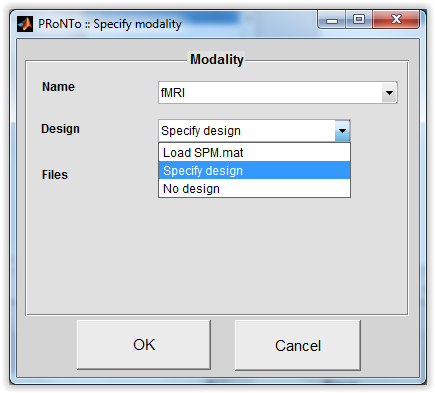
\includegraphics[height=3in]{images/Figure4.png}
   \caption{Data and design graphical user interface. The design menu in the modality window (when one uses the select by subject option) allows one to load a previously specified design from an SPM.mat file, create a new design or simply select no design, which usually applies to modalities where there is no experimental task, such as MRI or PET.}
    \label{Fig2.4}
  \end{center}
\end{figure}

\paragraph{Design} To create a new design one selects the option `Specify design' as explained in the previous paragraph (Figure \ref{Fig2.4}). This will then open another window (after choosing how many conditions you have) (Figure \ref{Fig2.5}). In this window one can then write the names, onsets, and durations of each condition. The units in which this information is read is specified below. There are two options `Scans' or `Seconds'. If the unit scans is selected, it is good to bear in mind that PRoNTo follows the convention, adopted in SPM, that the first scan is scan 0. In the durations field, one can introduce as many values as the number of onsets or just simply one value, which assumes the events all have the same duration. In this window there is also the option of introducing the Interscan Interval (TR), which is always read in seconds. 

One issue to have in mind when specifying the design is the following: if there are more scans than experimental events, these extra scans will not be used in later analyses. They are not deleted and the corresponding indexes can be found in the PRT structure: \\ PRT.group(g).subject(s).modality(m).design.conds(c).discardedscans. 

\begin{figure}[!h]
  \begin{center}
      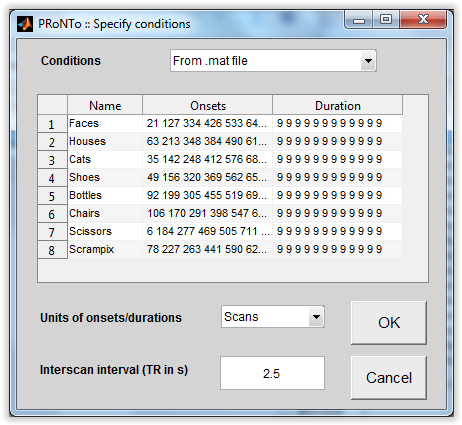
\includegraphics[height=3.5in]{images/Figure5.png}
   \caption{Data and design graphical user interface. The `specify conditions' window is available from the modality interface when the user chooses to enter the data by subjects and clicks `specify design'. This window is used to enter the conditions (names, onsets and durations) as well as the units of design, TR and covariates. }
    \label{Fig2.5}
  \end{center}
\end{figure}


\paragraph{Modify design}

The user can later modify a design by loading a PRT.mat in the Data and Design window. Please note that if feature sets or models have been previously computed, they will be discarded if changes are performed to the dataset. If the user wants to keep those, he/she should change the directory before saving any modification to the design. 

After loading a previously saved PRT, any change can be performed: subjects, groups or files can be added or removed. If the design needs to be modified, a right-click (ctrl+left-click in Mac) on the name of the concerned modality proposes to re-open the modality definition window. To review or modify the onsets/durations/blocks, the user can access their definition via the `specify design option'. Similar right-clicks (ctrl+left-click in Mac) allow renaming groups or subjects.

To modify the HRF parameters (delay or overlap), there is no need to load the PRT in Data and Design. Loading it within the Data Review allows the user to keep all previously computed feature sets and models. However, if the HRF parameters are changed, feature sets have to be computed anew since they do not correspond to the modified design. Changing the desired parameter (e.g. replacing `0' by `6') and hitting the `return' key updates the PRT directly in terms of scans selected for modelling. 
Please remember to keep an eye on the Matlab window, since important information are displayed on the workspace!

\paragraph{Files} Finally, independent of the way the user entered the information (by subjects or scans) the `Files' option allows one to choose which image files to use (Figure \ref{Fig2.6}). This will open another window that shows all image files available in each directory. These can be selected one by one or all at once, by using the mouse's right button on the right panel of the window (or shift key).

\begin{figure}[!h]
  \begin{center}
      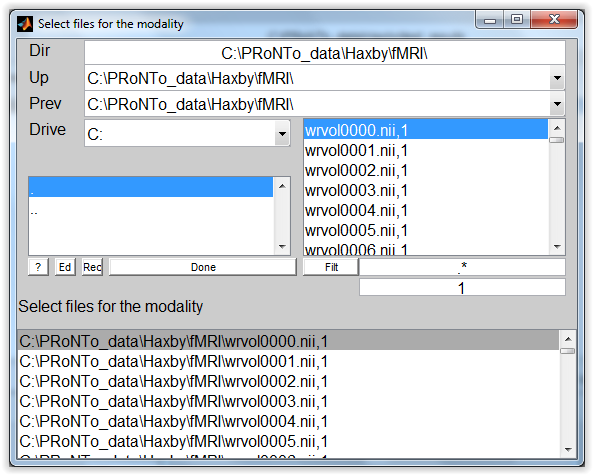
\includegraphics[height=3.2in]{images/Figure6.png}
   \caption{This window is called when one clicks `Files' and is used to select the scans/images for each subject/modality.}
    \label{Fig2.6}
  \end{center}
\end{figure}

All that is needed for each group, subject and modality has been specified and can now be viewed on the main window (Figure \ref{Fig2.7}) under each panel. The last panel shows which files have been entered for each modality and can be modified directly (click Modify). When Modify is clicked and no files are then selected all the previous files are deleted! Figure \ref{Fig2.7} shows how the data and design interface should look like once all the fields have been specified (using select by subject).
The design and files for each modality can also be modified by right clicking on the modality name in the modality panel. This option can be useful to visualise the design (onsets and durations) that has been previously entered and change it if necessary. For instance, one can check the design of the first subject and if changes are needed these can then be replicated for all other subjects as explained above.

\begin{figure}[!h]
  \begin{center}
      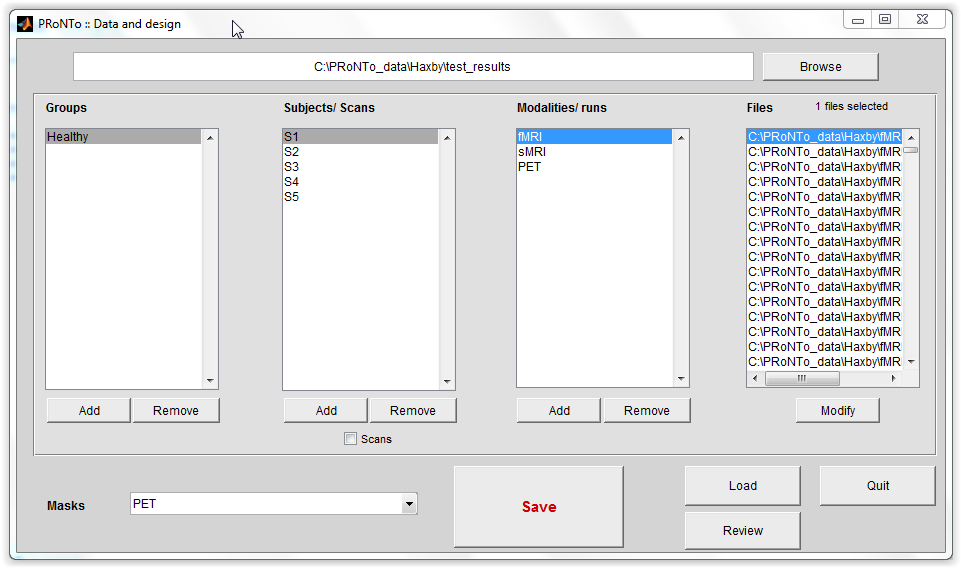
\includegraphics[height=2.85in]{images/Figure7.png}
   \caption{Data and design graphical user interface. After filling in all the fields using the select by subject option (the select by scans case is very similar) the data and design interface should look like this example figure.}
    \label{Fig2.7}
  \end{center}
\end{figure}


\subsection{Masks}

This popdown menu on the bottom of the main data and design window is where the user enters a binary image mask for each modality. This mask can be previously created by the user or simply chosen from a list of default masks available in the masks directory of PRoNTo. Every modality has to have a mask, which can be the same for all modalities. This is a first-level mask and is used simply to optimise the prepare feature set step by discarding all uninteresting features, such as voxels outside the brain. Later in the analysis one can choose another mask (second-level mask) that is more relevant to the scientific question and that can, for example, restrict the analysis to certain areas of the brain. To specify the mask one needs only to select the modality and then enter an image file. If the modalities have not yet been created, then one can create the modalities here, which will then appear in the modality panel.

\textbf{Important note}: If the first-level mask overlaps with areas that do not have values (e.g. either 0 or NaN) in the specified images, those areas will still be taken into account for further analysis. This might affect the results if those areas are not the same across images (typically, performance will be lower). We therefore advise the user to check the overlap between the first-level mask and his/her data. In most cases, this will not be needed, but for the acquisition of e.g. specific slices, this is recommended. We provide a script to update the mask automatically for beta images derived from a SPM GLM analysis (see \ref{chap:intro}, Inputs and preprocessing).

\subsection{Review}

The `Review' button allows one to review the data and design for each modality (Figure \ref{Fig2.8}). On the top right is the information relative to the number of groups and modalities that have been entered. The plot on the left displays the number of subjects per group. This is particularly important to check if the design is too unbalanced in terms of subjects. Then on the bottom right panel is the design information for each modality (if the selected modalities have an experimental design). Here, the user can view the number of conditions and can also edit the parameters that control the HRF delay and overlap (as explained above). The user can change the default value of 0 seconds and the effect is immediately seen on the number of scans plotted on the left (number of selected scans and number of discarded scans for each condition). The higher the value of the HRF peak and overlap, the higher the number of discarded scans. One can also read on the main Matlab window information regarding which group/subjects have had some scans discarded. The information below the HRF parameters corresponds to the interval between successive scans before and after the HRF delay/overlap correction. These values also change according to the changes entered in the boxes above. Please note, as mentioned in the section `Modify design', that information regarding the PRT being updated after changing the HRF parameters is written on the main Matlab window. 
%Again if you have previously computed feature sets and models, you have to recompute them because they do not correspond to the data anymore (changing the HRF delay and overlap parameters changes the data). 
% NOTE:AR-edit
Once again, if you have previously computed feature sets and models, you have to recompute them because they do not correspond to the data anymore (changing the HRF delay and overlap parameters changes the data). 
The information regarding which scans have been removed or not from the analysis can be found in the PRT structure: \\
{\tt PRT.group(g).subject(s).modality(m).design.conds(c).hrfdiscardedscans}.

\begin{figure}[!h]
  \begin{center}
      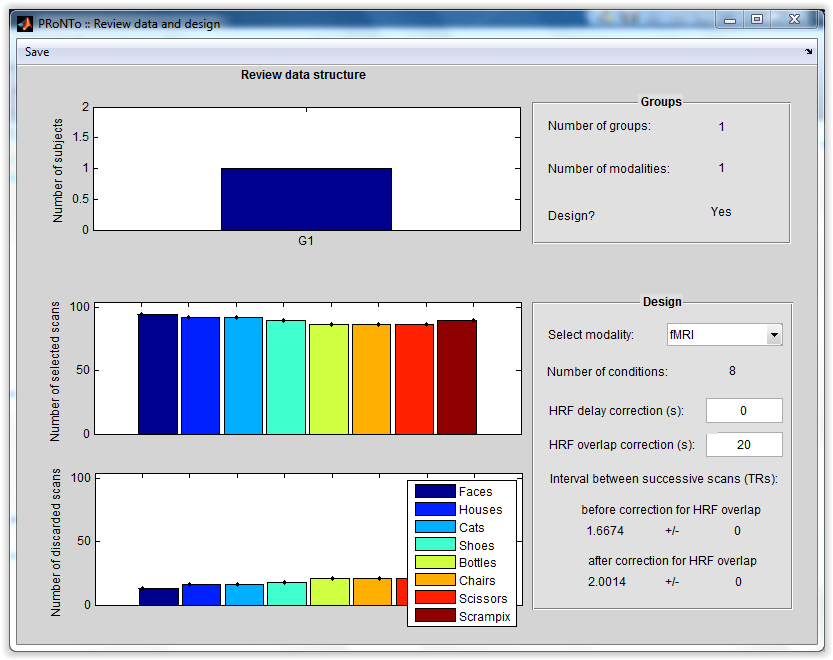
\includegraphics[height=4in]{images/Figure8.png}
   \caption{Data and design graphical user interface - `Review' window. This window allows the user to check the data and design, including the number of subjects per group. It also allows the user to change the HRF delay and overlap parameters that control the number of discarded scans (appropriate only for modalities such as fMRI). When there is no experimental design only the top plot and information is shown.}
    \label{Fig2.8}
  \end{center}
\end{figure}

\subsection{Load, Save and Quit}

The `Save' button allows the user to create the {\tt PRT.mat} file with the PRT structure containing all the information that has been specified here (Figure \ref{Fig2.7}). Incomplete information cannot be saved. At least one group should have all the required fields so that {\tt PRT.mat} can be created. `Load' allows the user to load the data and design information from a previously saved PRT.mat. The user can then edit the fields and update PRT by clicking again the `Save' button. It's very important to click `Save' because all the other steps in the analysis rely on the PRT structure. Without this structure one cannot proceed. However, when the {\tt PRT.mat} contains fields that have been added by the `Prepare feature set' or other modules, if the Save button is clicked, these fields will be deleted. The option `Quit' allows the user to leave the interface without saving the information. This is also the case when the user closes the window without first using the Save button.

\section{{\tt matlabbatch} interface}

The `Data and Design' module in the {\tt matlabbatch} is called either by first typing `prt' and clicking the `Batch' button or by typing `prt$\_$batch'. The user can then find on top of the batch a PRoNTo menu and under this menu the first module corresponds to the data and design module.

The options presented in the `Data and Design' GUI, mentioned above, are all available in the {\tt matlabbatch} interface (Figure \ref{Fig2.9}). However, there are a few things in the batch that differ from the GUI. One issue to note here is that, when using the batch one needs to be very careful with the names of the modalities specified for each subject (or using select by scans) and specified for each mask. The number of modalities should be exactly the same for each group and subject and the names should be consistent between groups/subjects and correspond to the names of the modalities under the masks field. In the GUI the names are made automatically consistent. The names of the conditions should also be the same across subjects and will be later used to define classes in the `Specify model' batch module.

Another issue is the HRF delay and overlap correction values. In the batch, the user can directly alter these values (instead of having to use the `Review' window) but the default is 0 seconds and should be changed (e.g. to 6 seconds) for modalities that depend on the HRF, such as fMRI.

As mentioned in the Introduction, the batch job can be saved as a .mat, and loaded again whenever needed, or as a .m that can be edited using the Matlab editor. This is a powerful tool that can make the specification of the data and design a lot easier and quicker, for example by editing and scripting existing batch files (for further information see the {\tt matlabbatch} chapter below).

\begin{figure}[!h]
  \begin{center}
      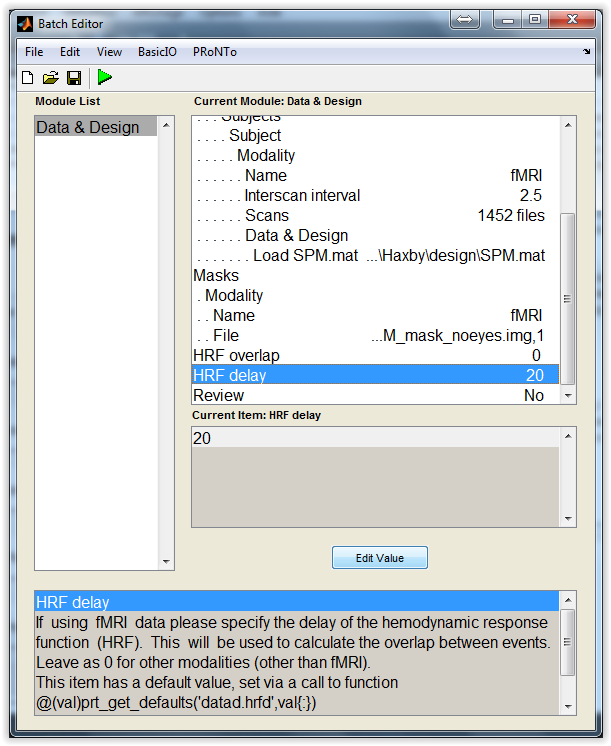
\includegraphics[height=4in]{images/Figure9.png}
   \caption{Data and design module in {\tt matlabbatch}. The {\tt matlabbatch} contains two extra options relative to the Data and Design interface. These options allow one to specify the delay and overlap of the HRF response (in the GUI it can only be changed in the `Review' window), and which are then used to determine the number of discard scans.}
    \label{Fig2.9}
  \end{center}
\end{figure}

% $Id: gui_preproc.tex 395 2011-11-17 22:34:59Z cphillip $
%
% Written by Jessica Schrouff
%_______________________________________________

\chapter{Prepare feature set}
\label{chap:PrepFeat}
\minitoc

\section{Introduction}
%===============
\label{sec:prep_intro}
One of the main inputs of a machine learning algorithm consists in a $N_{samples} \times N_{features}$ data matrix, containing the values of selected features for each sample. 
This matrix can either be input directly into the machine or be used to compute a ``similarity matrix", or kernel, of size $N_{samples} \times N_{samples}$, which is then input into the classification/regression algorithm [see ``kernel trick" \cite{Hofmann2008,Aizerman1964}]. PRoNTo computes a linear kernel (i.e. dot product) between the samples.
The `Prepare Feature Set' step computes both the feature and linear kernel matrices from one or more modalities, as defined in the previously built dataset (see chapter \ref{chap:DataDesign}). 
It allows detrending the features in the case of time series (such as fMRI) and scaling each image by a constant factor (input by the user) in the case of quantitative modalities (such as PET). Masks can be specified to perform the classification/regression on specific voxels only (e.g. Regions of Interest).

Multiple runs entered as different modalities (e.g. modality 1 is `fMRI\_run1', modality 2 is `fMRI\_run2',...) can be concatenated in terms of samples during this step. 
The images from different runs should then have the same number of features (i.e. selected voxels). In addition, version 2.0 allows to build multiple kernels, either from multiple modalities, or based on different anatomically labelled regions as defined by an atlas. In the case of multiple modalities, it is required that the selected modalities have the same number of samples, i.e. images. 

\section{Methods and resources}
%========================

After the selection of the dataset and of which modality to include in the feature set (further referred to as FS), the toolbox accesses each image, i.e. it gets the value of the voxels which are comprised in the first level mask selected for that modality (mask specified at the data and design step, see chapter `Data and Design'). 
This access is performed by `blocks' of features, not to overload the RAM memory. In the case of time-series, the user can specify detrending
methods and parameters to apply to the time course of each feature. Methods comprise a polynomial detrending (parameter: order of the polynomial) or
a Discrete Cosine Transform high-pass filter (SPM, parameter: frequency cutoff in seconds). An example of a linear detrending (polynomial detrending
of order 1) is shown in Fig. \ref{fig:lindetrend}.
\begin{figure}[!h]
  \begin{center}
      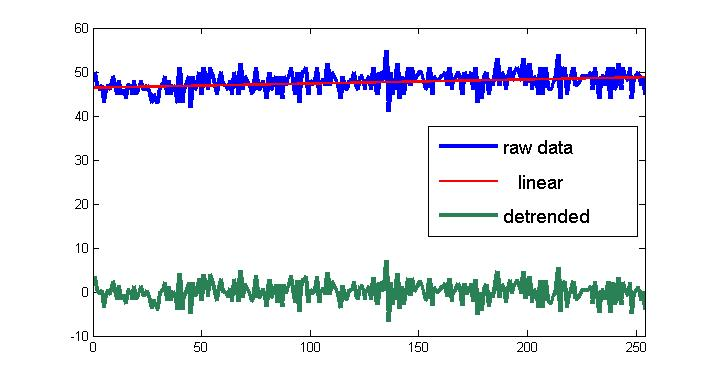
\includegraphics[height=6cm]{images/fig1_lindetrend.png}
   \caption{Example of detrending: the original signal over time of one feature (in blue) was approximated by a polynomial of order 1 (red line), which was then substracted from the original signal to give the detrended signal (in green).}
    \label{fig:lindetrend}
  \end{center}
\end{figure}

For each modality, the (detrended) features are then written in a file array (SPM, with a `.dat' extension), on the hard drive (in the same directory as the dataset). Please note that in the case of large datasets, this operation may require many Gb of free space on the hard drive and long computational times. Therefore, if the first condition can't be fulfilled, we recommend the use of external drives for the whole analysis. Regarding the computational expenses, we tried to minimize their effect by computing the features only once per modality: when preparing other feature sets using the same modality and detrending parameters, the built file array will be accessed for the next steps. 

{\bf Be careful} that using the same modality but different detrending methods and/or parameters will force the re-computation of the file array for the considered modality. In the same way, changing the dataset ({\tt PRT.mat}) from directory might lead to the re-computation of the feature sets if the file arrays were not moved accordingly. 

From the feature set(s), a linear kernel can then be computed. Different options can be specified:
\begin{itemize}
\item All scans/ All conds: In `all scans' the kernel matrix will be computed between all scans within the time series of all subjects and in `all
conds' the kernel matrix is computed only between the scans corresponding to the specified conditions of interest (see `Data and Design'). By default, the toolbox will use all scans to compute the kernel. With large datasets however, computational expenses can be reduced by selecting the last option. 
\item Scaling: allows the specification of constant values to scale each scan. The user has to enter a .mat containing a variable called `scaling' and of the same size as the number of scans in that modality. In case of quantitative modalities such as PET, this step is required since it insures the convergence of the machine learning algorithm.
\item Additional mask for selected modality: this option allows  the specification of a `second-level' mask, which would for example define Regions of Interest (ROIs) on which the classification/regression can be performed. In this case, the voxels used to compute the kernel (and only the kernel) would be the ones contained in both the first and second-level masks. Therefore, using one first-level mask and two second-level masks would create two kernels but only one file array.
\item Build one kernel per region: starting from version v2.0, PRoNTo allows to build one kernel per region as defined by an anatomically defined atlas, specified by the user\footnote{The atlas corresponds to a mask, except that the value of the voxels in each defined area correspond to a unique value, e.g. all voxels in fusiform have the value 3, and all voxels in orbito-frontal have the value 50.}. One atlas (Anatomical Automatic Labelling, AAL) is provided in \textit{your PRoNTo folder/atlas}. Atlases can be generated easily through SPM, or manually by the user. There are no constraints on how regions are built, as long as all the voxels within each region have a specific integer value. The toolbox will identify the different regions based on the values in the voxels. Each region will then act as a second-level mask and one kernel will be built for each region. The kernels are all saved in a same feature set and will then all be used at the modelling stage.
\end{itemize}

These options are performed at the kernel level only. This means that any change in one of these options would lead to the computation of a new kernel but not to the (re)computation of the file arrays. The use of different second-level masks or scaling parameters can therefore be easily envisaged.

ProNTo version 2.0 allows to build multiple kernels. These kernels can be derived from multiple modalities or from multiple regions of interest as defined by an atlas within each modality. These two options are not mutually exclusive and it is also possible to build multiple kernels within each modality and then combine those modalities as multiple kernels. The number of kernels would hence become \textit{number of modalities} $\times$ \textit{number of regions}. In the same way, it is possible to concatenate multiple runs of an experiment while building one kernel per region.

The {\tt PRT.mat} structure saves all information linked to the file arrays in a {\tt fas} field (standing for ``File Array Structure''), which size corresponds to the number of selected modality in all feature sets. The selected options and the link to the kernel (saved on the disk as a .mat) are stored in a {\tt fs} field (standing for ``Feature Set''), which size corresponds to the number of feature sets defined by the user.

\section{Graphical User interfaces}
%==========================

After clicking on the ``Prepare Feature Set'' button in the main interface (see Fig. \ref{fig:mainprep}), a second window will appear (Fig. \ref{fig:FSmainl}), allowing the user to select a saved PRT.mat, to name the FS and to define the number of modalities which should be included in the FS. 
\begin{figure}[!h]
  \begin{center}
      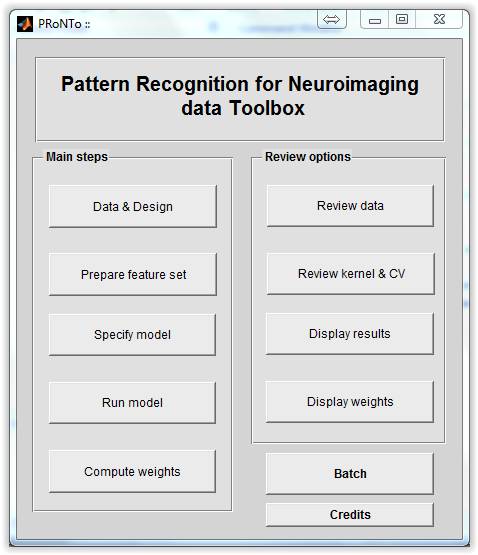
\includegraphics[height=7cm]{images/fig2_main_prt.png}
   \caption{Main interface: button to launch the 'Prepare Feature Set' step.}
    \label{fig:mainprep}
  \end{center}
\end{figure}

\begin{figure}[!h]
  \begin{center}
      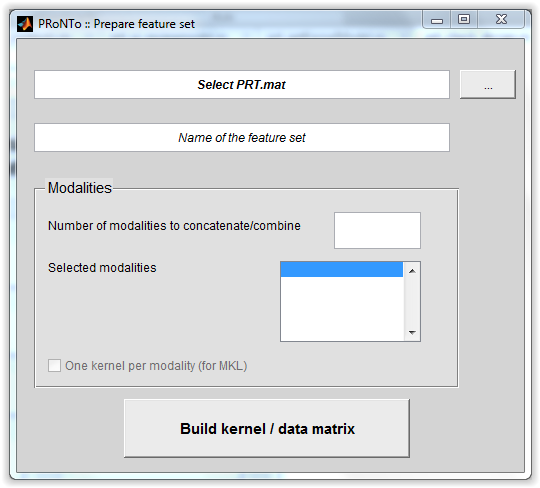
\includegraphics[height=9cm]{images/prt_ui_feature_set.PNG}
   \caption{Interface of the `Prepare Feature Set' step. Top: Dataset selection: type the full name (with path) or browse to select the dataset to prepare. Feature set name: Type the FS name, which will be used to save the kernel as a .mat on the hard drive. Modalities: Number of modalities to select with the list containing the names of the modalities included in the FS (no user interaction possible). A checkbox allows to build one kernel per modality if multiple modalities are present/have been selected in the FS. Build kernel/data matrix: builds the feature set and kernel(s).}
    \label{fig:FSmainl}
  \end{center}
\end{figure}

To define the number of modalities to include, the user should click in the appropriate edit box, type the number and then `return'. This will launch a third window (Fig. \ref{fig:modFS}), allowing the specification of the different options and parameters for each modality. When the dataset contains only one modality, this window is launched directly and (Fig. \ref{fig:FSmainl}) is filled automatically expect for the feature set name.
\begin{figure}[!h]
  \begin{center}
      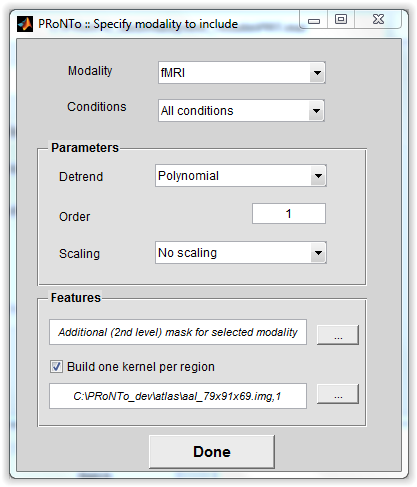
\includegraphics[height=7cm]{images/prt_ui_feature_set_modality.PNG}
   \caption{Specification of options and parameters for each modality. Modality: Select the modality name from a pull-down menu. Conditions: choose to build All scans or All conditions. Parameters: Detrend to perform with its parameter, as well as Scaling of the scans or not. Features: Selection of a second-level mask and/or of an atlas to build one kernel per region.}
    \label{fig:modFS}
  \end{center}
\end{figure}

In this third window, the user has to choose which modality to include based on its name (first pull-down menu) and  which scans to use to build the kernel (all or only those linked to the design). All other options are facultative. The first panel refers to operations to perform on the features:
\begin{itemize}
\item the detrending parameters: by default, the parameter is set to `No detrending'. However, we recommend to perform a detrending in the case of
time series data such as fMRI (and only in that case). When selecting polynomial, the `order' parameter will appear, with a default value of 1.
Changing this value will increase the order of the polynomial used to fit the data. If `Discrete Cosine Transform' is selected, the editable
parameter corresponds to the cutoff frequency (in seconds) of the high-pass filter. Please note that, when including more than one run (`modality') into a feature set, nothing will prevent the user from using different detrending methods/parameters. We however highly recommend to use a consistent detrending in the same FS.
\item the scaling: `no scaling' is the default option. However, when dealing with quantitative modalities such as PET, the user should provide one value per scan, stored in a vector in a .mat file under the variable name 'scaling'.
\end{itemize}

As previously mentioned, the detrending is performed before the features are saved in the file array, while the scaling is performed only when building the kernel.

The second panel allows to select a subset of the saved features to build the kernel. Two options are available:
\begin{itemize}
\item the specification of a second-level mask: type the full name (with path) of the mask or browse to select the mask image. When left empty or untouched, voxels are selected from the first-level mask specified in the data and design step. Otherwise, voxels within both the first and second-level masks will be selected to build the kernel.
\item the building of one kernel per region: when selecting this option, the user should load an atlas which defines regions in terms of their anatomy (in MNI space). Each region will then act as a second-level mask and one kernel will be built for each region. 
\end{itemize}

When working with Graphical User Interfaces (GUIs), some messages might appear in \matlab workspace. These can display information about the operations currently performed or explain why the toolbox does not do as the user expected (e.g. when a file could not be loaded or if information was input in a wrong format). Therefore we strongly encourage the user to have a look at \matlab prompt when using GUIs.

\section{{\tt matlabbatch} interface}
%=======================

The {\tt matlabbatch} system allows the input/selection of all parameters and options aforementioned. Just note that the batch is based on the names of the modalities and/or conditions. Therefore, for the batch to work properly, names should be consistent across all steps, starting from data and design to the model specification and running. The hierarchy for the case of a feature set containing one fMRI modality is displayed in (Fig. \ref{fig:batchFS}). For this feature set, we chose to load an atlas, and build multiple kernels based on the regions it defines.

\begin{figure}[!h]
  \begin{center}
      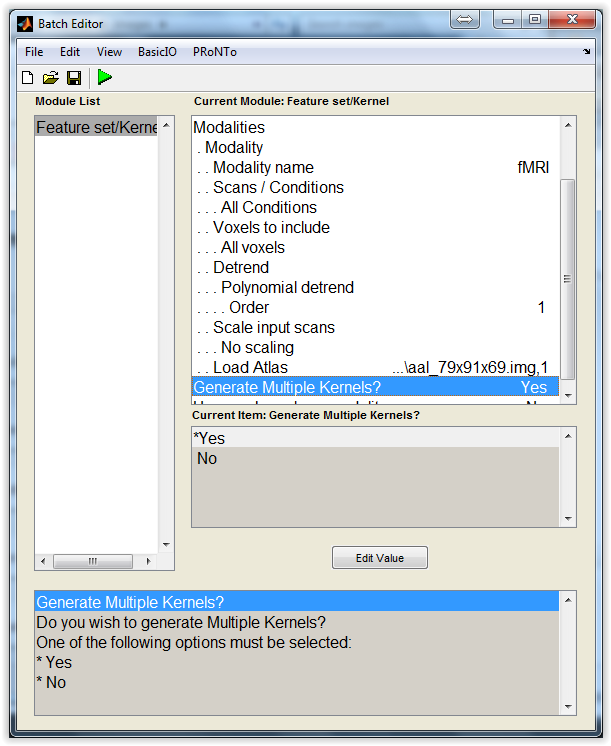
\includegraphics[height=10cm]{images/fig5_batchFS.png}
   \caption{{\tt matlabbatch} GUI for feature set building.}
    \label{fig:batchFS}
  \end{center}
\end{figure}

{\bf Important note:} Defining all important steps in one batch and running that batch will overwrite the {\tt PRT.mat} previously created and thus delete the links between the {\tt PRT.mat} and the computed kernel(s) and feature set(s). The file arrays would then be recomputed each time the batch is launched. For large datasets, we therefore recommend splitting the batch in two parts: a data and design and prepare feature set part and a second part comprising the model specification, run model and compute weights modules. This would indeed allow changing, e.g. model parameters, without recomputing the feature sets and kernels. 

% $Id: gui_amodel.tex 395 2011-11-17 22:34:59Z cphillip $
%
% Written by A Marquand, updated by J. Schrouff for v2.0
%_______________________________________________

\chapter{Model Specification and Estimation}
\label{chap:ModelCrossV}
\minitoc

\section{Introduction}

The specification of a model is the core step of the pattern recognition pipeline and  entails setting up the combination of the different components making up the analysis. For example, model specification is where you select which data features to use as input (i.e. a feature set), the type of prediction to perform (e.g. classification or regression), which machine learning algorithm to employ (e.g. support vector machines, Gaussian processes, ...), which cross-validation strategy to employ (e.g. leave one subject out, leave one run out, ...) and which operations or manipulations to apply to the kernel before the algorithm is trained. The framework provided by PRoNTo is highly flexible and supports most types of pattern recognition analysis typically performed in neuroimaging. This chapter provides an overview of each of the components making up a model in PRoNTo. The presentation will focus on the user interface although it is important to note that the batch system provides several advanced options not available in the user interface (described further).

\section{Beginning a model specification}

To begin a model specification with the PRoNTo user interface, select `Specify model' from the main PRoNTo window. This will launch the model specification window (Figure \ref{fig_specify_model})

\begin{figure}[!h]
\begin{center}
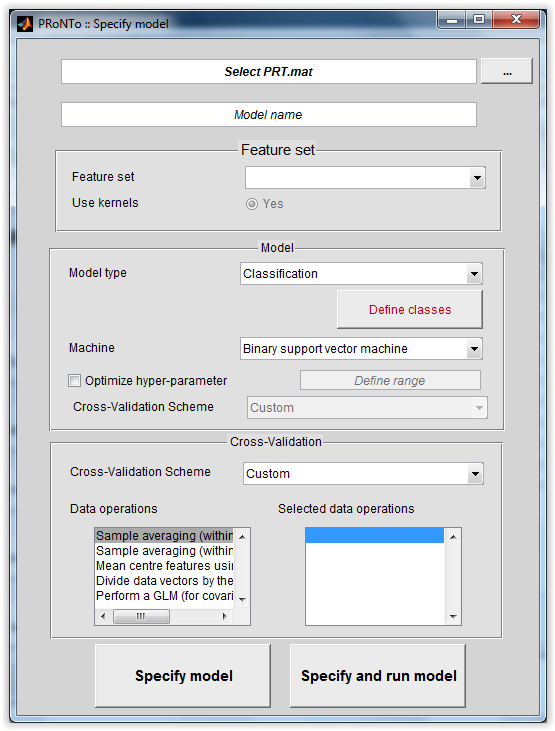
\includegraphics[height=3.5in]{images/prt_ui_model.png}
\caption{Model specification graphical user interface}
 \label{fig_specify_model}
\end{center}
\end{figure}

Next, select the \texttt{PRT.mat} containing your experimental parameters. Note that at least one feature set must be defined in this structure before a model can be created. See chapter \ref{chap:PrepFeat} for details on constructing feature sets.

Enter a unique name to identify the model, which is used internally in PRoNTo, by the batch system and for display purposes. It is a good idea to select a meaningful but short name (without spaces). \textbf{Note:} the \texttt{PRT.mat} data structure retains a permanent record of all models created but if a model with the specified name already exists in the \texttt{PRT.mat} data structure, it will be automatically overwritten.

\section{Feature set}
The drop-down list entitled `Feature set' will be populated once a \texttt{PRT.mat} containing one or more feature sets is selected. Select the appropriate feature set from the drop-down list. Note that a single feature set may contain more than one data modality (see chapter \ref{chap:PrepFeat}), which can be combined to build multimodal classification and regression models (e.g. L1-Multiple Kernel Learning models). This might also be useful if more than one run/session is available for each subject, in which case each run could be input as an independent modality in the data and design step and a single-subject classifier might be specified using leave-one-run-out cross-validation. 

In the current release of PRoNTo, only kernel machines are supported via the user interface. The capability to support non-kernel techniques will be added in a future release. Thus, the `Use kernel' radio button should always be set to true.

\section{Model type / pattern recognition algorithm}
In this part of the model specification input form, select the pattern recognition algorithm to employ (referred to in PRoNTo as a `machine'). In the current release, three classification algorithms are supported (binary support vector machines, Gaussian processes (binary and multiclass) and L1-Multiple Kernel Learning) and four multivariate regression methods (Gaussian process regression, kernel ridge regression 
\footnote{Kernel ridge regression is equivalent to a \emph{maximum a posteriori} approach to Gaussian process regression with fixed prior variance and no explicit noise term} , relevance vector regression and L1-Multiple Kernel Learning). 

\textbf{Note:} if a feature set contains multiple kernels (either from regions of interest or based on different modalities) but the selected classification/regression technique is a single kernel method (e.g. SVM or KRR), the kernels will first be summed before entering the classification/regression phase. This corresponds to concatenating the features before building the kernel. For regions of interest in a single modality, the summed kernel is hence equivalent to a whole brain model.

The PRoNTo user interface provides a mechanism for flexible definition of which components of the data design should be used for each classification or regression model. Note that this will not necessarily be the whole experiment; for example, in a complex fMRI experiment there may be several groups, each containing multiple subjects, each in turn having multiple experimental conditions (e.g. corresponding to
different subprocesses of a cognitive task). In such cases, it is usually desirable to ask several different questions using the data, such as discriminating between groups for a given experimental condition (``between group comparison"), discriminating between experimental conditions for a fixed group (`between-task comparison') or training independent pattern recognition models for different subsets of subjects. All of
these can be easily defined via the user interface by clicking the `Define classes' button (for classification) or `Select subjects/scan' (for regression).

\subsection{Classification}

The class selection panel is displayed in figure \ref{fig_specify_classesC}. First, define the number of classes, noting that some classification algorithms (e.g. support vector machines) are limited to binary classification, while other classification algorithms (e.g. Gaussian processes) support more than two classes. Enter a name for each class - again, it is a good idea to make these names informative but short. Notice that immediately after the number of classes has been specified, the group-, subject- and condition selection panels are greyed out. To enable them, simply select one of the classes from the drop-down menu.

For each class, select the subjects and conditions (if any) that collectively define that class. It is possible to select multiple experimental
conditions in the same class, but this complicates model interpretability and potentially also model performance (since by definition
conditions are not identically distributed). If a condition or subject is erroneously selected, click on it in the `selected subject(s)' or
`selected condition(s)' panel and it will be removed from the list. The performance of classification models is evaluated based on measures such as total accuracy, class accuracies and positive predictive values (representing the sensitivity and specificity). 

\begin{figure}[!h]
\begin{center}
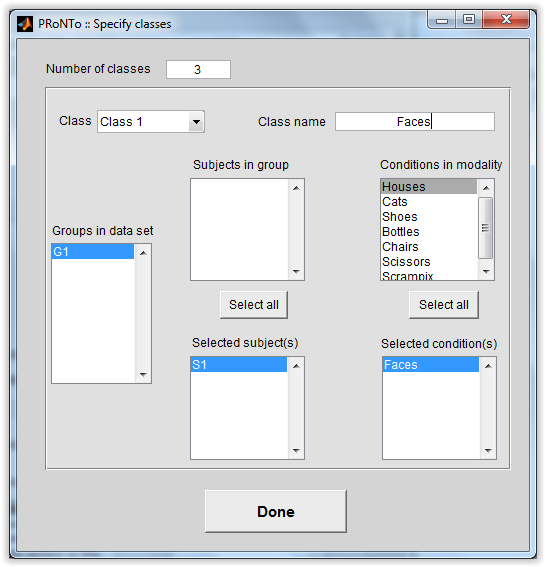
\includegraphics[height=3.5in]{images/prt_ui_model_classes.PNG}
\caption{Subject / condition selection panel for classification models}
 \label{fig_specify_classesC}
\end{center}
\end{figure}

\subsection{Regression}

Regression is a generic term for all methods attempting to fit a model to observed data in order to quantify the relationship between two groups of variables. Traditionally in neuroimaging massively univariate strategies (e.g. GLM) have been largely used, where data for each voxel are independently fitted with the same model. Statistics test are used to make inferences on the presence of an effect at each voxel (e.g. \emph{t-test}).  Multivariate regression, on the other hand, takes into account several input variables (voxels) simultaneously, thus modelling the property of interest considering existing relations among the voxels.

Although most studies exploring predictive analyses in neuroimaging have been related to classification, regression analysis has aroused interest in neuroscience community for its ability to decode continuous characteristics from neuroimaging data. This approach has potential to be used when the examples (patterns) can be associated to a range of real values. The objective is to predict a continuous value instead of predicting a class to which the example belongs. These values usually refer to demographic, clinical or behavioural data (as age, blood pressure or scores resulting from a test, for example). For validation, different metrics can be used to compute the agreement between the predicted values and the actual ones, such as Pearson's correlation coefficient (r) and Mean Squared Error (MSE).

The specification of which subjects and scans to include in regression models is similar to that for classification, see Figure  \ref{fig_specify_classesR} and for the purposes of model specification in PRoNTo, regression can be thought of as a classification problem with a single class. In the current release, regression is only supported if there is a single scan per subject (e.g. structural images or beta images from a GLM analysis). In a future release it will be possible to perform regression where an independent regression target is supplied for each trial, block or condition. To perform a regression, the regression targets are specified during the design stage. It is important to emphasize that in the current implementation, regression is only supported using the "select by scans" option (see chapter \ref{chap:DataDesign}).  

\begin{figure}[!h]
\begin{center}
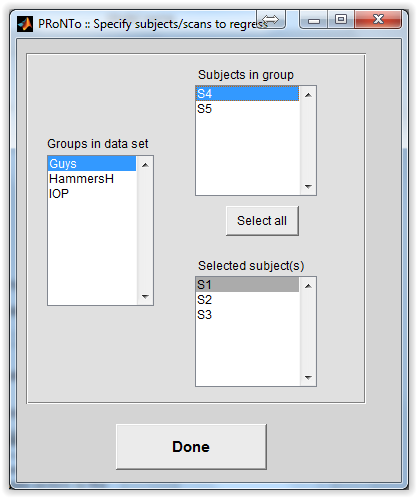
\includegraphics[height=3.5in]{images/prt_ui_model_regression.PNG}
\caption{Subject / condition selection panel for regression models}
 \label{fig_specify_classesR}
\end{center}
\end{figure}

\subsection{Hyper-parameter optimization}

From PRoNTo version 2.0, it is possible to optimize hyper-parameters of the machine learning models. For example, the soft-margin (a.k.a. C) hyper-parameter in
SVM can be optimized, using a nested cross-validation scheme. In this case, there are two loops in the cross-validation scheme. The inner loop is used for parameter optimization and the outer loop is used for assessing the model's performance. More specifically, the data is divided into training and testing sets according to the cross-validation scheme selected (outer loop). For each fold of the outer loop the training set is further divided into training and testing sets according to the cross-validation scheme selected (inner/nested loop). The inner loop is used to train and test the model with each value of the hyper-parameter specified by the user. The parameter leading to the highest performance in the inner/nested loop (balanced accuracy for classification and Mean Squared Error for regression) is then used in the outer loop. For each fold of the outer loop, the model is trained using the 'optimal' value of the hyper-parameter and tested on the data that was left out (and which was not used for parameter optimization). This nested CV procedure can lead to different values of the hyper-parameter to be selected in each fold. These are stored in the outputs of the model and can be reviewed in the `Display Results' panel.

Optimizing the hyper-parameter might lead to improved results compared to fixed values. This will usually depend on the number of features selected to model the data: for example, for whole brain models based on SVM classifiers, with many more features than images/trials, it is reasonable to assume that changing the hyper-parameter won't affect the model performance significantly due to the high dimensionality of the data with respect to the number of examples. However, when using (e.g.) regions of interest (in a second-level mask or in a MKL model), the ratio between the number of features and the number of examples will be much smaller. In this case, different values of the hyper-parameter might lead to different decision functions and optimizing the hyper-parameter is desirable.

Performing a nested cross-validation can be computationally expensive. For computational efficiency, PRoNTo allows to specify different cross-validation schemes for the `outer' and the `nested' CV\footnote{For example, the outer CV could have more folds, to use as much data as possible in each fold for prediction (e.g. leave-one-out), while the nested CV would not need as many folds to select the `optimal' value of the hyper-parameter (e.g. k-folds CV).}. 

In the current version of PRoNTo, the soft-margin parameter can be optimized for SVM and for MKL (classification and regression). In the same way, it is possible to optimize the $\lambda$ ridge parameter for KRR. If no value is provided, those parameters will take the values $0.01, 0.1, 1, 10, 100$ and $1000$, i.e. $10.^{[-2:3]}$.

\section{Cross-validation}

In the final part of the specify model input form, select the type of cross-validation to employ. Cross-validation is a crucial part of the
pattern recognition modelling and is used to assess the generalisation ability of the model and to ensure the model has not overfit to the data. Typically this is done by
partitioning the data into one or more partitions: a `training set', used to train the model (e.g. fit parameters) and a `testing set' used to assess performance on unseen data. By repeatedly repartitioning the data in this way, it is possible to derive an approximately unbiased estimate of the true generalisation error of the model. 

The most common cross-validation schemes in neuroimaging applications are leave-one-subject out (LOSO; exclude one subject for testing, train with the remaining), leave-one-run-out (LORO; leave one fMRI run out for testing, train with the remainder) and leave-one-block-out (LOBO; leave out a single block or event and train with the remainder). LOSO is suitable for multi-subject designs, while LORO and LOBO are suitable for single subject designs, where the former is better suited to designs having multiple experimental runs and the latter is appropriate if there is only a single run. The current release of PRoNTo supports each of these, and also supports leave-one-subject-per-group-out (LOSGO), which is appropriate if the subjects in each group are paired or for repeated measures experimental designs. Versions 1.1 and later allows k-fold cross-validation for each of the available schemes. This means that the user specifies the number of folds (`k') and that the data is partitioned according to that number. For example, specifying $k=4$ will use 25\% of the data to test the model, and 75\% to train it. Note: $k=1$ splits the data in half, training the model on the first half and testing on the second, i.e. there is no circular partitioning.

In version 2.0, a GUI allows the user to fully specify his/her cross-validation scheme. First, a `basis' needs to be specified (Figure \ref{fig_customCV_basis}). Three options are available: 

\begin{itemize}
\item Load a .mat containing a previously computed CV matrix (needs to contain the variable `CV').
\item Select a basis from the pop-down list (contains the same options as for the outer CV).
\item Specify the number of folds.
\end{itemize}


\begin{figure}[!h]
\begin{center}
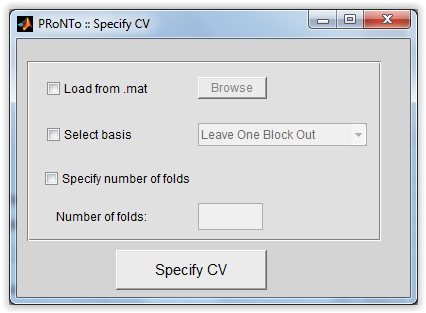
\includegraphics[height=4cm]{images/prt_customCV_basis.PNG}
\caption{Specify basis to build custom cross-validation}
 \label{fig_customCV_basis}
\end{center}
\end{figure}

When an option has been selected, a new window will appear (Figure \ref{fig_customCV}). The top panel of this window is a table that can be edited. Each row refers to a trial/image selected in the definition of the classes (or to perform regression on). Each column represents a fold. For each column, the different trials can have a value of 2 (test set), 1 (train set) or 0 (unused in this fold). Setting a whole fold to 0 takes it out of the CV matrix. Note: it is possible to change the value of multiple trials by changing the value of the last trial to modify, then shift-select the first one to modify. This also works across folds. The bottom panel displays the structure of the data selected for further classification or regression, along with a preview of the built CV matrix.

\begin{figure}[!h]
\begin{center}
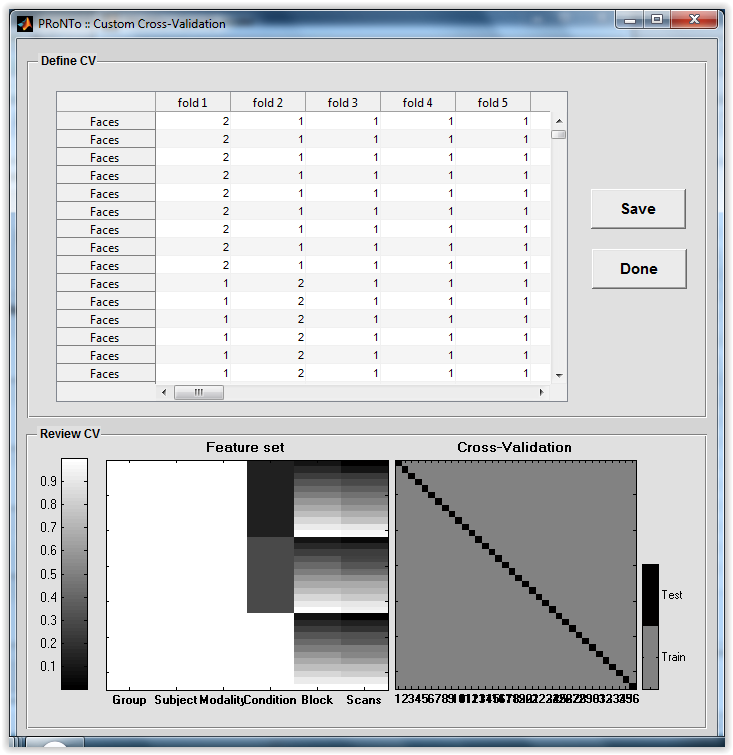
\includegraphics[height=9cm]{images/prt_customCV.PNG}
\caption{For each fold, specify which images/trials are part of the training and test set, or are unused}
 \label{fig_customCV}
\end{center}
\end{figure}

The resulting CV matrix can be saved in a .mat, alongside the PRT (name: \textit{model name\_ CV.mat}). This matrix can loaded as a custom CV in the batch, if exactly the same trials were selected for modelling. \textbf{Note:} The `custom' CV option is not available as a nested/inner cross-validation scheme. 

Information concerning the cross-validation structure is stored internally in matrix format, and can be visualised by clicking `Review Kernel and CV' from the main ProNTo window (see \ref{fig_reviewCV} for an example). In the left panel, this figure indicates which group, subject, modality and condition each scan in the feature set belongs to. On the right, each cross-validation fold (partition) is displayed as a separate column and each scan is colour coded according to whether it is in the training or testing set (or if it is unused).


\begin{figure}[!h]
\begin{center}
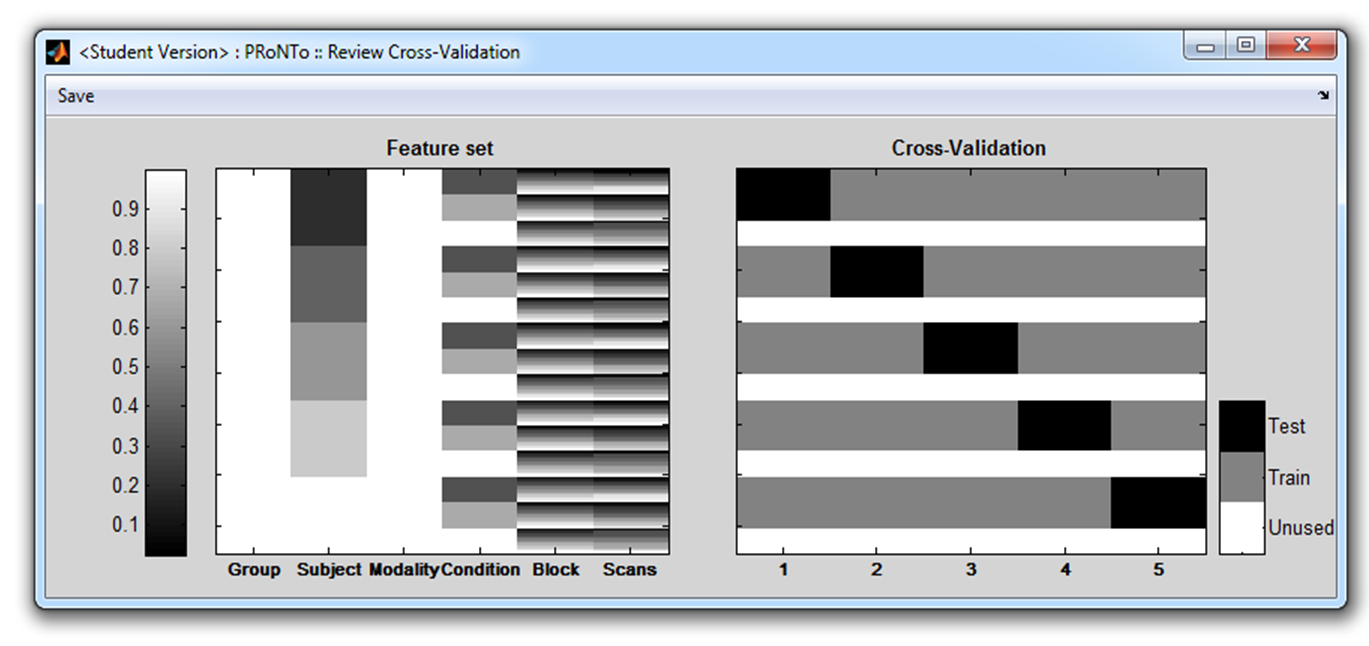
\includegraphics[height=2in]{images/prt_ui_reviewCV.png}
\caption{Review cross-validation matrix}
 \label{fig_reviewCV}
\end{center}
\end{figure}

It should be emphasised that the type of cross-validation selected should be appropriate for the experimental design. For example, it is nonsensical to select a leave-one-subject-out cross-validation approach for single subject designs. It is also important to ensure that the training and testing sets are completely independent to avoid the cross-validation statistics becoming biased. This is particularly important for fMRI, where successive scans in time are highly correlated. For example, if a leave-one-block-out approach is employed and the blocks are too close together then the independence of the training and testing set will be violated, and the cross-validation statistics will be biased (technically this is governed by the autocorrelation length of the fMRI timeseries and the temporal blurring induced by the haemodynamic response function). This can be avoided if care is taken to ensure that overlapping scans are discarded from the design (see chapter \ref{chap:DataDesign}), but it is a very important issue, and the user should still be careful to ensure that cross-validation folds are sufficiently far apart in time (especially for LOBO cross-validation).

During this part of the model specification, it is also possible to select one or more operations to apply to the data. Each of these operations is defined below:

\begin{enumerate}
\item \textbf{Sample averaging (within blocks):} constructs samples by computing the average of all scans within each block or event for each subject and condition. 
\item \textbf{Sample averaging (within subjects):} constructs samples by computing the average of all scans within all blocks for each subject and condition.
\item \textbf{Mean centre features using training data:} subtract the voxel-wise mean from each data vector.
\item \textbf{Divide data vectors by their norm:} scales each data vector (i.e. each example) to lie on the unit hypersphere by dividing it by its Euclidean norm.
%\item \textbf{Regressing out covariates:} regresses out the covariates entered for each subject/image (entered `by scans') from the kernel. \textbf{Note:} This operation is actually performed without taking into account the separation between training and test sets. A new formulation of this operation, taking into account the division of train and test, is currently in development and will be implemented as soon as possible.
\end{enumerate}


%(except for the GLM)
A crucial point to note is that all operations are embedded within the cross-validation structure such that they are applied independently to training and testing sets. This prevents a very common mistake in pattern recognition from occurring, whereby parameters are computed using the whole data set prior to cross-validation. Observing a complete split between training and testing sets during all phases of analysis ensures that accuracy measures are an appropriate reflection of the true generalisation ability of the machine and are not biased because of improper applications of preprocessing operations to the entire dataset.

Other points to note include: (i) the order of operations is potentially important. For example, subtracting the mean then dividing each data vector by its norm is not the same as performing the operations the other way around. (ii) operations (1) and (2) have no effect if no design is specified or for events with a length of one TR.

At a minimum, we recommend that features should be mean centered over scans during cross-validation. In addition, for multiple kernel learning, we advise the user to normalize each kernel. This will compensate for the fact that different kernels might be computed from examples/samples with different number of features (e.g. different regions contain different numbers of voxels).

The different operations selected for a specific model can then be reviewed using the `Review Kernel and CV' (starting from version 2.0). The selected operations will be listed below the kernels (`Show kernel').

\section{Specify / Run model}

Using the GUI, it is possible to either `Specify' the model, or `Specify and Run' the model. The first option saves all the parameters of the model in the PRT structure. This information can be found in \texttt{PRT.model(\textit{m}).input}, where \textit{m} is the index of the model. The second saves all the parameters of the model and then runs the model. In this case, the inputs, which include the cross-validation matrix, the target values or labels, and the machine (e.g. binary SVM, Gaussian Process, etc.), are fed to the estimation routines, which will then add to the PRT an output field (\texttt{PRT.model(\textit{m}).output}) containing the estimated parameters, statistics, and other information from the learning process.

In some cases (e.g. multiple models to run or models with nested CV and/or slower machines), it would be desirable to estimate models later on (e.g. just before lunch break or at the end of the day). The `Run model' option allows to select multiple models and run them one at a time automatically (Figure \ref{fig_run_model}). The first thing that needs to be done using this window is to specify which PRT we would like to work with. PRoNTo will then read the available models from this structure and display the list of models on the left panel. These models can be selected (the selected models will show on the right panel) by clicking each model individually or by clicking the `Select all' button in the middle of the panels. Finally, to estimate the model(s), one needs only to click the bottom button `Run model(s)'.

\begin{figure}[!h]
\begin{center}
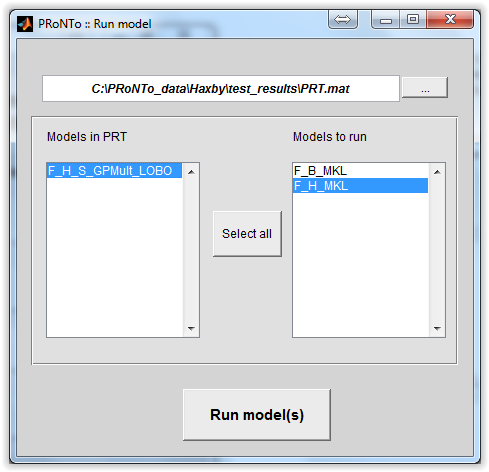
\includegraphics[height=5cm]{images/prt_run_model.PNG}
\caption{Choose models to be estimated}
 \label{fig_run_model}
\end{center}
\end{figure}

It is useful to have a look at what is displayed in the \matlab command space when the model is being estimated. Information such as the number of folds can help double-check that everything is going as expected. Furthermore, if some options were specified (e.g. using a feature set with multiple kernels) that are not available at the modelling step (e.g. to be modelled with SVM), warnings will be displayed, as in Figure \ref{fig_ws_matlab}.

\begin{figure}[!h]
\begin{center}
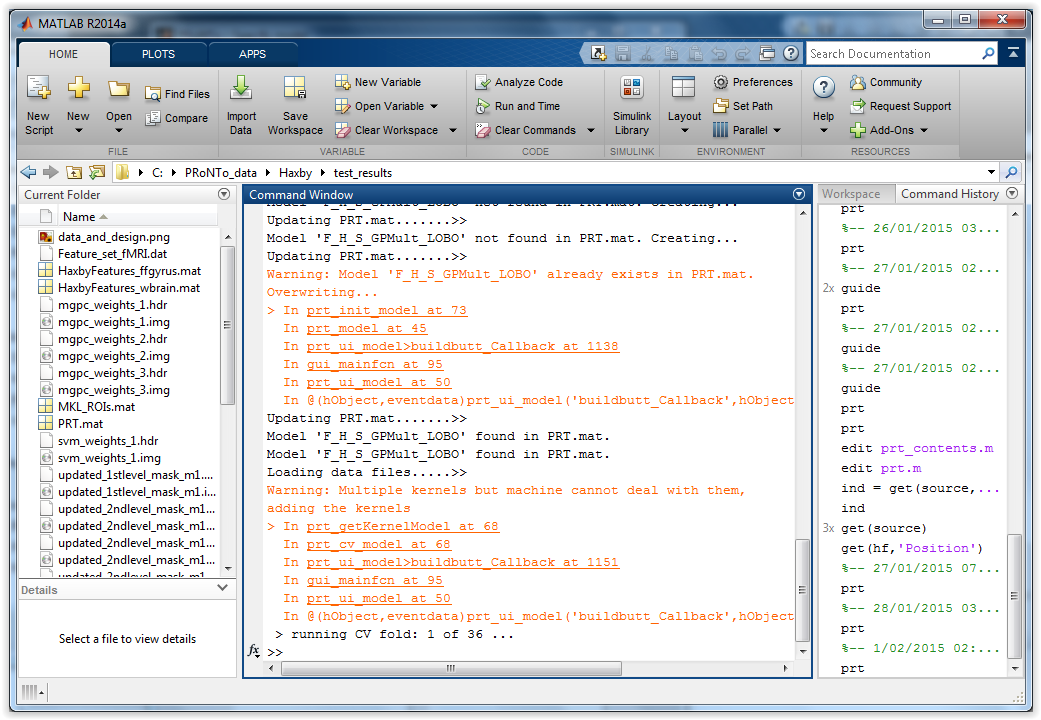
\includegraphics[height=8cm]{images/matlab_workspace_model.PNG}
\caption{\matlab workspace displaying warnings when kernels are added}
 \label{fig_ws_matlab}
\end{center}
\end{figure}

\textbf{Important note:} multiple kernel feature sets can be modelled using any machine. For machines not supporting multiple kernels, these will first be added before the model is estimated. This corresponds to concatenating the features from the different regions and/or modalities.

\section{Batch interface}

The batch module provides all the functionality provided in the user interface and allows complex analyses to be scripted in advance. As noted,
the batch module also provides functionality not available in the user interface. The most important difference is that the batch module allows
customised \matlab \ functions to be used as prediction machines. This functionality allows PRoNTo to be easily extended to allow many types of
classification and regression algorithms not provided under the current framework. This can be achieved by selecting `Custom machine' under the
`Model Type' heading. This allows a function name to be specified (i.e. any \texttt{*.m} function in the \matlab \ search path). The behaviour of this custom machine can then be controlled by a free-format argument string. See the developer documentation and the examples in the \texttt{machines/} subdirectory of the PRoNTo distribution for more information. Another important difference between the batch and user interfaces is that mean centering data vectors across scans is enabled by default in the batch. Also, flexible CV is available in the batch only in the form of `load a .mat'. This .mat must contain a variable called `CV', specifying the CV matrix for the selected trials/images.

An example of the batch window for model specification is provided in figure \ref{fig_batch_model}.

\begin{figure}[!h]
\begin{center}
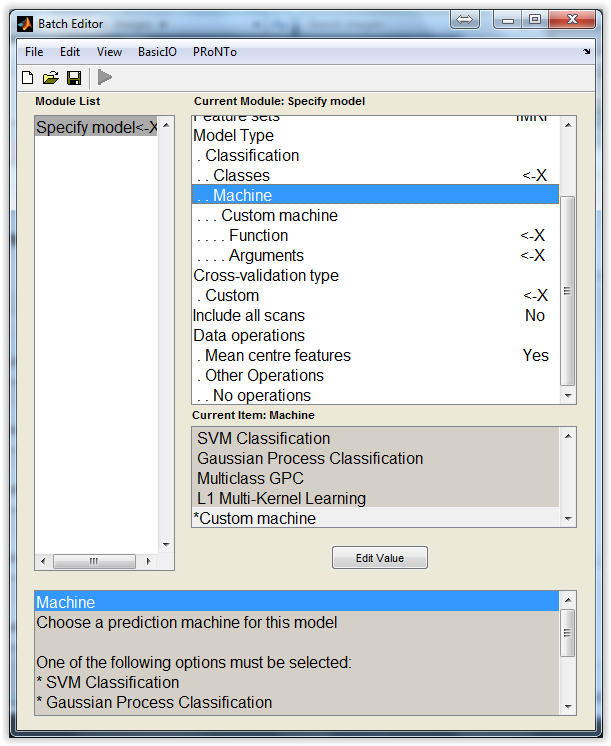
\includegraphics[height=3.5in]{images/prt_batch_model.PNG}
\caption{Batch interface to specify a model}
 \label{fig_batch_model}
\end{center}
\end{figure}

As displayed in Figure \ref{fig_batch_model}, the batch does not allow to specify and run the model directly. Instead, the user had to add a `Run model' module. The batch has the advantage of allowing to perform permutations along model estimation (option available in the `Display results' window in the GUI). Furthermore, it is possible to save the predictions and the balanced accuracy (for classification) for each permutation, to perform further statistical tests if needed. The `Run model' batch module is presented in Figure \ref{fig_batch_runmodel}. \textbf{Note:} Dependencies on the model name are available when performing a `Model specification' followed by a `Run model' module.

\begin{figure}[!h]
\begin{center}
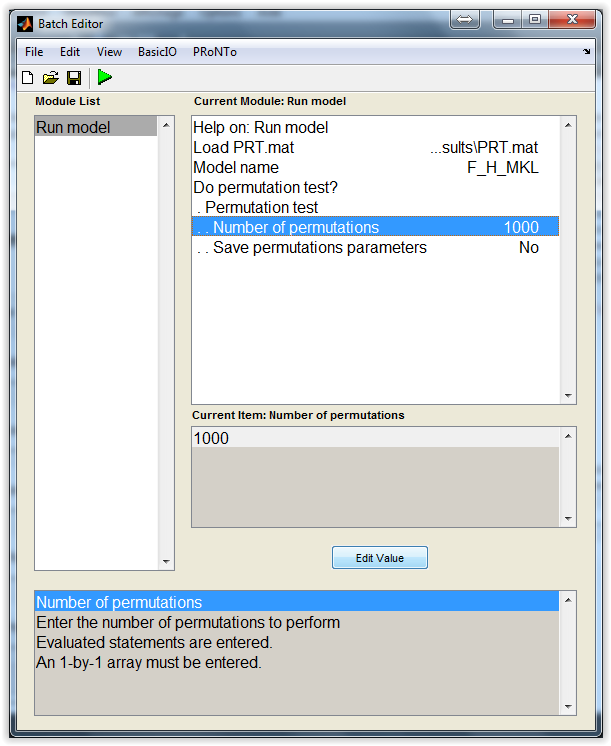
\includegraphics[height=3.5in]{images/prt_batch_runmodel.PNG}
\caption{Batch interface to run a model}
 \label{fig_batch_runmodel}
\end{center}
\end{figure}


% $Id: gui_bmodel.tex 395 2011-11-17 22:34:59Z cphillip $

\chapter{Computing Feature and Region Contributions}
\label{chap:ComputeWeights}

\minitoc

\section{Introduction}

The previous module allows the user to specify one or more models. These include the machine to be used, the cross-validation scheme and the classification/regression problem. The estimation of those models led to predictions on unseen/test data (in each fold), from which measures of performance of the model can be derived.

In addition, as PRoNTo uses linear models it provides the option of recovering the model weights in the original feature (voxel) space, and transforming the weights vector into an image, or map. These maps contain at each voxel the corresponding weight of the linear model (together defining the optimal decision function), and which related to how much this particular voxel contributed to the classification/regression task in question. The weights can later be displayed using the `Display results' module (described below).

Furthermore, the MKL machine estimates contribution of each kernel to the final decision function. This means that there will
be one value per region of interest as defined by an atlas and/or per modality (depending on how multiple kernels were built).
Therefore, it is possible to build maps at the region level, in addition to the maps at the voxel level. Regions/modalities
can then be ranked according to their contribution. Since L1-MKL is a sparse algorithm (i.e. only some kernels will have a non-null contribution to the model), this eases model interpretation.

\section{Methods}

The output of the linear kernel models in PRoNTo include the coefficients of the dual representation, i.e. the coefficients of the training examples. These coefficients are then multiplied by the training examples to obtain the model weights. The vector of model weights has the same dimensions of the original voxel space, and can therefore be converted to a 3D image. This computation is done for each fold. The resulting 3D images for all folds are then assembled into a single 4D NIFTI file with dimensions [3D x (number of folds + 1)], where $1$ corresponds to an extra 3D image with the averaged weights over all folds. The NIFTI file is saved in the same directory as PRT.mat. In the case of multi-class classification, one image will be built for each class, the index of the class being saved in the image name (e.g. \textit{image\_ name\_ c1.img}). In the case of multiple modalities being considered as multiple kernels (i.e. not concatenated in samples), one image will be built for each modality, the modality name being appended to the image name.

In addition, it is possible to build an image containing the contributions of each region of interest as defined by an atlas (same dimensions as for the voxel weight images). Two options are available:

\begin{itemize}
\item Contributions of kernels estimated through MKL: In this case, the contributions of each region to the model are derived from the contributions of each kernel. This option is available for MKL modelling of feature sets containing multiple kernels based on ROIs defined by an atlas.
\item Summarizing the weights according to ROIs: If a whole brain feature set was used, or if the kernels were added to perform single kernel modelling (e.g. SVM, GP, KRR, RVR), it is possible to select an atlas and summarize a posteriori the weights in each anatomically defined ROI. The contribution of each region is then simply the sum of the absolute values of the weights within that region, divided by the number of voxels in that region (see \cite{Schrouff2013a} for details).
\end{itemize}

In both cases, the contribution of each region is divided by the total contribution of all regions. The derived values can then be seen as percentages of contribution of each region to the decision function. The contributions can be ranked, leading to a list of regions sorted by descending contribution to the model. This list can also be computed if multiple modalities were built and used in an MKL model. In this case, each modality has a contribution to the model, that can be normalized and a sorted list can be derived.

Furthermore, for MKL models - which are sparse in the number of kernels contributing to the model - a bar graph can be built, representing the number of kernels with a non-null contribution to the model. The same graph bar will depict the contribution of each region to the decision function in the case of summarized weights. In this case, the bar graph will not be sparse.

\section{Graphical user interface}

If the user wants to create images of the weights, using the GUI, the user first needs to click the `Compute weights' button
on the main PRoNTo window. This will launch the window shown in Fig \ref{CompWeights}. To estimate the weights and create the
weight maps the user needs to select a {\tt PRT.mat} file. The window is then divided in two panels: a `Feature weights' panel
and a `Atlas-based weights' panel. In the first panel, PRoNTo will show the list of available models, and the user can choose
one model for which to estimate the weights. If the selected model is the MKL modelling of ROI-based kernels, the `Atlas-based
weights' panel will be automatically updated, and the name of the selected atlas at the feature set step will appear.
Otherwise, those fields will stay blank. In the `Feature weights' panel, it is also possible to define the name of the created
image file, which is saved in the same directory as PRT.mat. Alternatively, if left empty, PRoNTo will name the file according to the model name, class (if multi-class machine) and/or modality (if MKL on modalities). The `Atlas-based weights' allows to estimate the contribution of each anatomically defined region to the model. If the model refers to an MKL machine estimated on kernels per region, the `Atlas name' field will be filled automatically and the contribution of each region is derived from the contribution of each kernel. If this is not the case (single kernel machine or feature set), an atlas should be loaded (using the browse option). The weights will then be summarized for each region a posteriori.

\begin{figure}[h!]
\begin{center}
	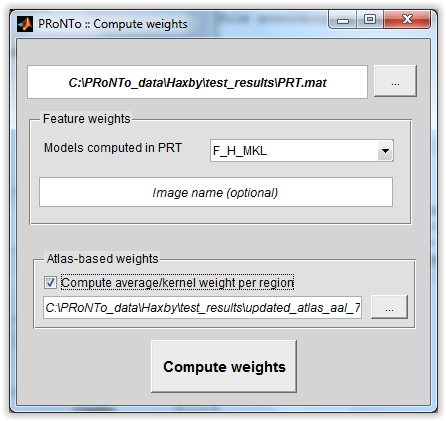
\includegraphics[height=7cm]{images/CompWeights.png}
	\caption{Weights computation GUI.}
	\label{CompWeights}
\end{center}
\end{figure}

\section{{\tt matlabbatch} interface}

The {\tt matlabbatch} module to compute the weights has the same options as the GUI. One main difference being that instead of listing the available models in a given PRT, it will ask for the name (string) of the model to be used. As for estimating models, the name of the model should be exactly the name given in `Specify model'. Another difference is that the batch allows to compute weight images for each permutation. In this case, only the average across folds will be saved in a nifti. This potentially allows for statistical tests to be performed on weights and/or on the derived ranking of the regions (for MKL modelling of anatomically defined ROIs).

\begin{figure}[h!]
\begin{center}
	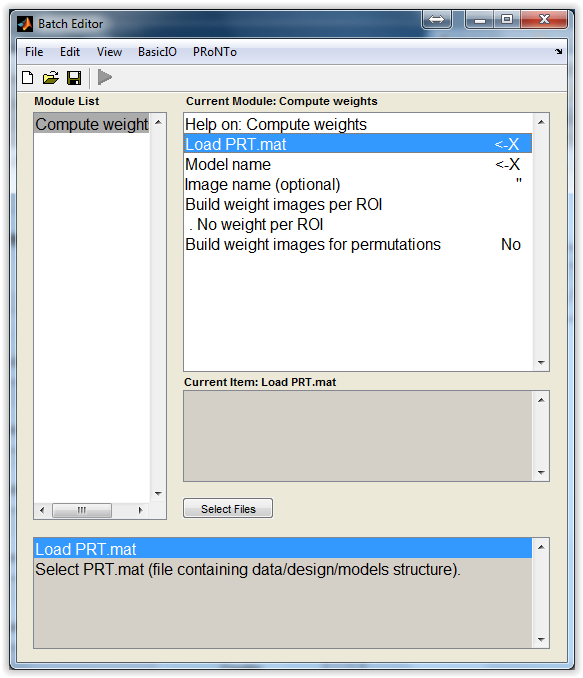
\includegraphics[height=7cm]{images/batchWeights.PNG}
	\caption{Weights computation GUI.}
	\label{batch_CompWeights}
\end{center}
\end{figure}

% $Id: gui_disres.tex 395 2011-11-17 22:34:59Z cphillip $
%
% Written by Jonas Richiardi, updated by J. Schrouff for v2.0
%_______________________________________________


\chapter{Display Model Performance}
\label{chap:DisRes}
\minitoc

\section{Introduction}

Once a machine (e.g. a classifier or a regression function) has been specified, 
its parameters have been estimated over training data, and its performance has been
evaluated over a testing set using cross-validation, it is necessary to examine the outcome
of the whole procedure in detail. The results windows enables the user to see the model's performance evaluated by different metrics.

Examining model output and parameters is helpful in diagnosing the potentially
bad performance of a particular model. For example, if the machine cannot perform above
chance, it could be due to an inappropriate experimental paradigm, noisy data, insufficient
amount of data, wrong choice of features,  or the wrong choice of machine. It is important to
recognise that any of these factors could cause the modelling to fail. 

Model performance can be reviewed using the `Display Results' GUI. Alternatively, all computed statistics are saved within the PRT structure, in the \texttt{PRT.model(m).output.stats} field, with \texttt{m}, being the index of the model to review.

\section{Launching results display}

Make sure all previous steps have been performed (Data and Design, Chapter~\ref{chap:DataDesign};
Prepare feature set, Chapter~\ref{chap:PrepFeat}; Specify Model and Run Model, Chapter~\ref{chap:ModelCrossV} ).

In the {\tt Review Options} panel of the main PRoNTo window, press {\tt Display Results}. At the `Select PRT.mat' window, navigate to where your {\tt PRT.mat} file is stored (using the left column), and select it. The main results window will open and look as represented in Figure \ref{fig_prt_ui_results_emptyWin}. In the {\tt Model} panel in the top-right corner, the list of models that have been successfully estimated will appear. Note: there will be a `beep' if one or more models were specified but not estimated (`Run model') and their name will appear in the command window.

\begin{figure}[h!]
\begin{center}
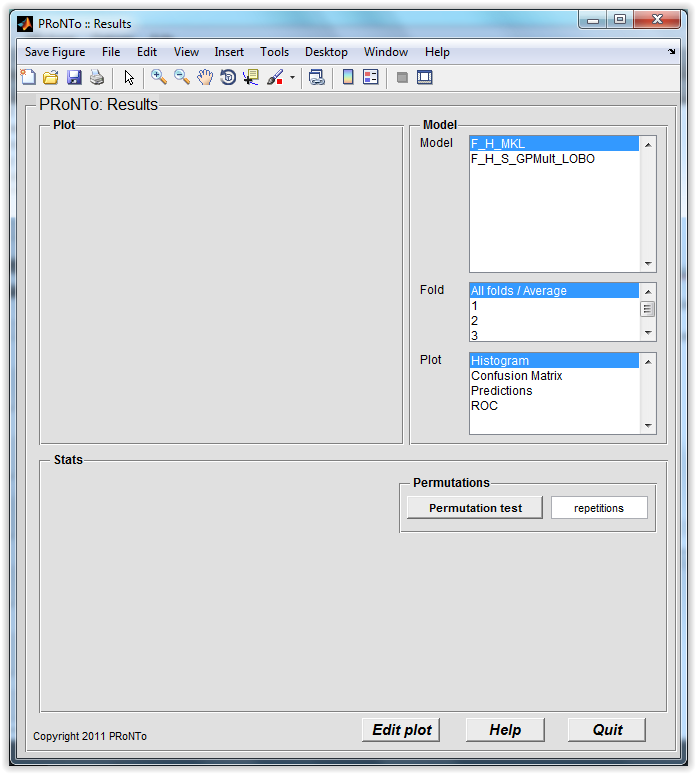
\includegraphics[width=10cm]{images/prt_ui_results_emptyWin.png}
\caption{Initial state of the results display main window.}
\label{fig_prt_ui_results_emptyWin} 
\end{center}
\end{figure}

\section{The main results display window}

The window is divided into three panels; going clockwise from top left to bottom left, they
are:
\begin{description}
\item[Plot]: This panel displays the plots for the various analyses that can be performed on
test results. With the exception of the confusion matrix plot, these cannot be interacted with.
\item[Model]: This panel allows the user to select the model to visualize, whether to visualize a
particular fold or all folds at once, and which plot to produce.
\item[Stats]: The {\tt stats} panel allows the user to visualize a variety of performance metrics (based on the selected fold), including accuracy statistics for classifiers and MSE for regression models. In addition, p-values for these metrics based on permutation tests can also be visualized.
\end{description}

To populate the `Plot' panel, first click on a model in the {\tt Model} selector, then on
`all folds' (or a particular fold) in the {\tt Fold} selector, and finally on a plot
in the {\tt Plot} selector. The next section details the plots available.

The window also comprises `Edit plot', `Help' and `Quit' buttons. The `Edit plot' button exports the displayed plot in an extra window, such
that it can be edited and easily saved. The `Help' button provides information on each panel of the window (not as detailed as in this
manual) and the `Quit' button closes the results window. In addition, the GUI menu comports a `Save figure' option (on the top left) that
acts as a `printscreen' of this window (with white background), which can be saved for records/publications.

\section{Analysing a machine's performance graphically}

Looking at a machine output's graphically can often yield insights into the performance
of the machine. In PRoNTo, plots are different for classification and regression.

\subsection{Classification}

\subsubsection{Predictions plot}

A prediction plot displays, for a particular fold (y-axis), the output value of the machine's
decision function for each test sample (x-axis, e.g., for a linear SVM, this could be $\mathbf{w}^T\mathbf{x}_i + b$,
for a probabilistic classifier this could be a posterior probability $P(\Omega=\omega | \mathbf{x}_i)$). The decision threshold is displayed by a vertical line at the centre of the plot.
A well-performing classifier will yield very different function values for samples of different
classes, i.e. samples from different classes will fall on different sides of the decision threshold. 
%By observing which fold have more or less overlapping function values, it is possible
%to understand which block / subject / condition might have a test distribution of features that
%departs from the training set. 
The inspection, in each fold, of the overlap of function values between classes, can help to identify which of the test blocks/subjects/conditions is atypical with respect to the training set.  
This plot is available for binary classification.


On the plot, each class is represented by a different marker and color, and indicated in the legend.
Figure \ref{fig_prt_ui_results_plots_pred} shows an example predictions plot. 

\begin{figure}[h!]
\begin{center}
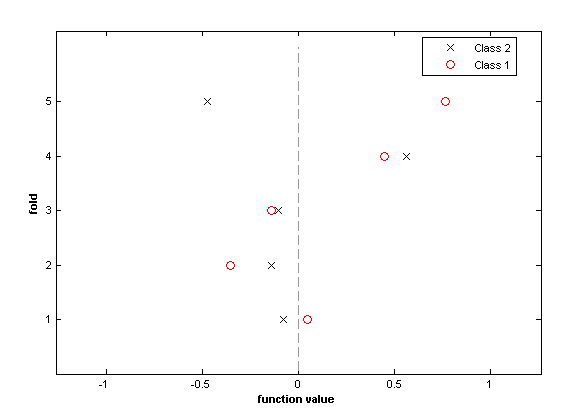
\includegraphics[height=6cm]{images/prt_ui_results_plots_pred.png}
\caption{Example predictions plot for a two-class problem modelled by an SVM.}
\label{fig_prt_ui_results_plots_pred}
\end{center}
\end{figure}

\subsubsection{Receiver Operating Characteristic (ROC) plot}

In two-class classification, there is always a trade-off between class 1
and class 2 errors. Indeed, a classifier predicting class 1 regardless of input
would have excellent accuracy on class 1, but bad accuracy on class2. This is also
known as the sensitivity / specificity trade-off. The 
ROC curve is a graphical depiction of this trade-off, showing how one error rate
varies as a function of the other. An ideal classifier would have an ROC passing
through the top-left corner. The area under curve (AUC) is a summary measure of 
classifier performance, where higher is better (1 represents perfect performance,
0.5 represents random performance). As with all summary measures,
the AUC is but one way of comparing performance of machines, and cannot be used alone
to declare a machine statistically significantly superior to another on a given dataset.

Figure \ref{fig_prt_ui_results_plots_ROC} shows an example of such a plot (Haxby dataset, Faces versus Houses, 4-folds nested CV, LOBO outer CV).

\begin{figure}[h!]
\begin{center}
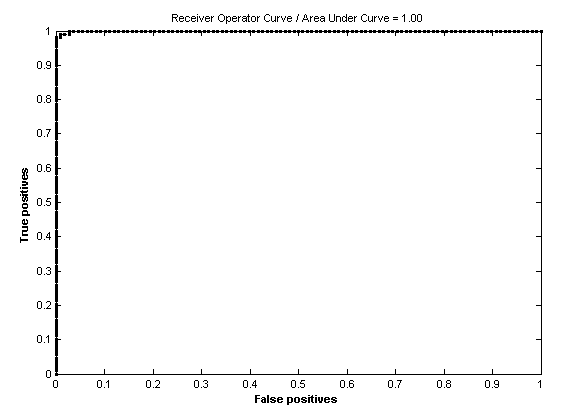
\includegraphics[height=6cm]{images/prt_ui_results_plots_ROC.png}
\caption{Example ROC curve for a two-class problem modelled by an MKL on ROIs.}
\label{fig_prt_ui_results_plots_ROC}
\end{center}
\end{figure}

\subsubsection{Histogram plot}

The histogram plot is a smoothed density version of the predictions
plot, showing how function values are distributed. A good classifier
would have minimal overlap between the densities. The error rate of the
classifier is proportional to the area of the overlap. The ROC curve can 
be thought of as the result of sweeping a decision threshold over the range
of functional values, and recording the joint sensitivity/specificity values
for each decision threshold setting. A typical linear SVM would have a decision
threshold at 0.

Figure \ref{fig_prt_ui_results_plots_hist} shows an example of such a plot for a binary classification (SPM EEG dataset, Faces versus Scrambled, LOBO CV).


\begin{figure}[h!]
\begin{center}
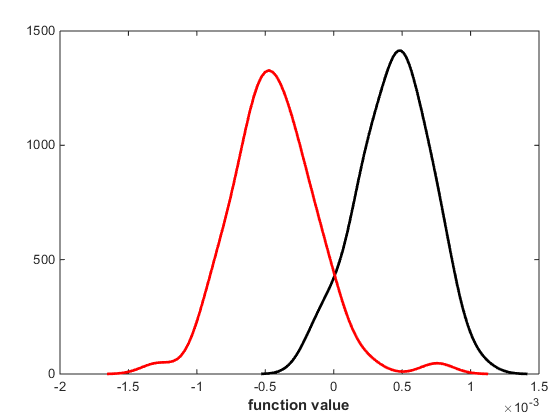
\includegraphics[width=8cm]{images/prt_ui_results_plots_hist.png}
\caption{Example function values histogram curve for a binary problem modelled by L1-MKL.}
\label{fig_prt_ui_results_plots_hist}
\end{center}
\end{figure}

\subsubsection{Confusion matrix plot}

The confusion matrix shows counts of predicted class labels $\hat{\omega}_n = f(\mathbf{x}_n)$ (in rows) versus true class labels $\omega_n$ (in columns). An ideal confusion matrix is diagonal: all predicted class labels correspond to the truth. Off-diagonal elements represent errors. It is important to check that none of the classes is
``sacrificed'' to gain accuracy in other classes - in other words, if all classes are equally
important to classify, no class should have more off-diagonal than on-diagonal entries. Many
summary statistics, including class accuracy, total accuracy, sensitivity, and specificity,
can be computed from the confusion matrix.

Figure \ref{fig_prt_ui_results_plots_confMat} shows an example of a confusion matrix (Haxby dataset, Faces versus Houses versus Scissors, LOBO CV).


\begin{figure}[h!]
\begin{center}
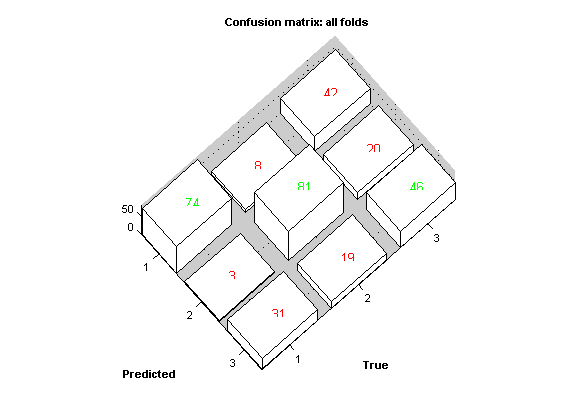
\includegraphics[height=6cm]{images/prt_ui_results_plots_confMat.png}
\caption{Example confusion matrix for all folds of a three-class problem modelled by GP.}
\label{fig_prt_ui_results_plots_confMat}
\end{center}
\end{figure}

\subsection{Regression}

\subsubsection{Predictions (scatter)}

This plot represents the predicted values (x-axis) against the real values or targets (y-axis). A perfect correspondence between targets and predictions would be represented by a diagonal on this plot. Figure \ref{fig_prt_ui_results_plots_predReg} displays such a plot for the prediction of age from sMRI images (IXI dataset, 15 images acquired across 3 centres).

\begin{figure}[h!]
\begin{center}
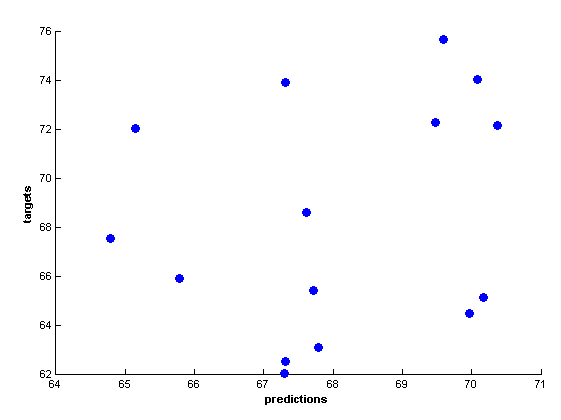
\includegraphics[height=6cm]{images/prt_ui_results_plots_predReg.png}
\caption{Example of scatter prediction plot on 15 data points modelled by KRR.}
\label{fig_prt_ui_results_plots_predReg}
\end{center}
\end{figure}

\subsubsection{Predictions (bar)}

This plot displays, for each image/subject, the target and the prediction in bar plots. An example plot is displayed in Figure \ref{fig_prt_ui_results_plots_bar} for the same model. 

\begin{figure}[h!]
\begin{center}
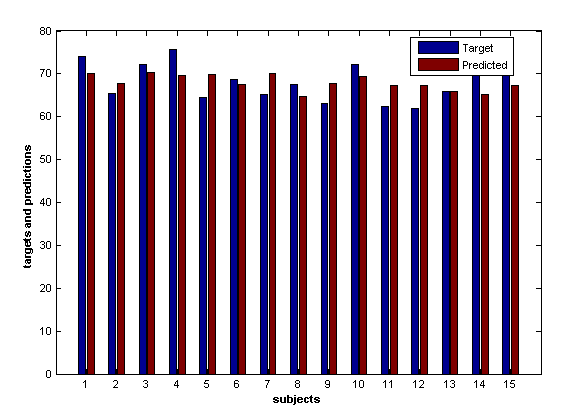
\includegraphics[height=6cm]{images/prt_ui_results_plots_bar.png}
\caption{Example of bar prediction plot on 15 data points modelled by KRR.}
\label{fig_prt_ui_results_plots_bar}
\end{center}
\end{figure}

\subsubsection{Predictions (line)}

This plot displays, for each fold, the target and the prediction, each in line plots. An example plot is displayed in Figure \ref{fig_prt_ui_results_plots_line} for the same model. 

\begin{figure}[h!]
\begin{center}
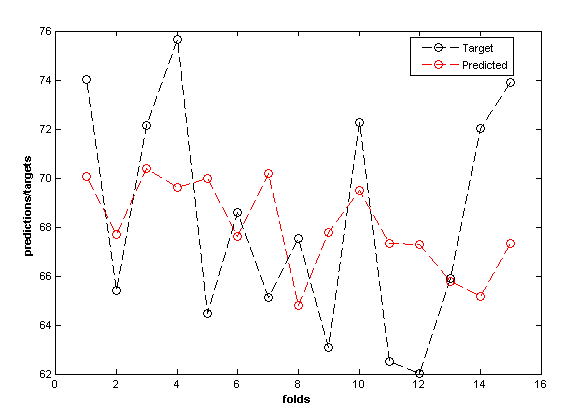
\includegraphics[height=6cm]{images/prt_ui_results_plots_line.png}
\caption{Example of line prediction plot on 15 data points modelled by KRR.}
\label{fig_prt_ui_results_plots_line}
\end{center}
\end{figure}

\subsection{Influence of the hyper-parameter on performance}

This plot will be present in the list if hyper-parameter optimization was performed. When displaying the average across folds, for each value of the hyper-parameter, it displays the average model performance (balanced accuracy for classification and MSE for regression, line on the plot) across nested folds, with an error bar representing the standard deviation of model performance. The frequency of selection of a hyper-parameter value (i.e. the number of times this value was returned as `optimal' to the outer CV fold) is represented with a gray bar plot on the right-side y-axis. An example of such a plot is displayed in Figure \ref{fig_prt_ui_results_plots_hyper} for the optimization of the soft-margin parameter in L1-MKL (Haxby dataset, Faces versus Houses, 4-folds nested CV, LOBO outer CV). When selecting a specific fold, this plot displays the model performance for each value of the hyper-parameter, and represents the optimal value (i.e. the one leading to highest performance) in red. 

\begin{figure}[h!]
\begin{center}
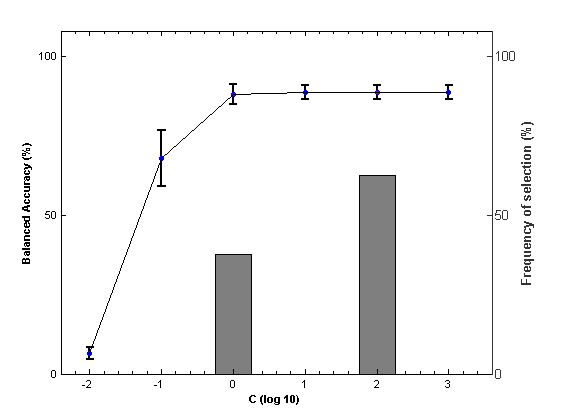
\includegraphics[height=6cm]{images/prt_ui_results_plots_hyper.png}
\caption{Example performance curve depending on the hyper-parameter value with frequency of selection of each hyper-parameter.}
\label{fig_prt_ui_results_plots_hyper}
\end{center}
\end{figure}

\section{Statistical analysis of a machine's performance}
\label{s:DisRes_stats}

One of the main questions to ask of a model is how precise its predictions are.
In regression, goodness-of-fit is often assessed via mean squared error and coefficient of determination ($R^2$). In classification, a common practice is to compute prediction accuracy, both for each class and for all test data. Once a specific performance metric has been obtained, it is also possible to obtain a p-value for the metric, reflecting
how certain we are that the result is not due to chance.

The statistics table gives a summary of the model's performance. Model performance is estimated differently for classification and for regression. In PRoNTo, classification performance is assessed using total accuracy (TA), balanced accuracy (BA), class accuracies (CA) and class predictive values. For regression, the goodness-of-fit is assessed based on the coefficient of determination ($R^2$), the mean squared error (MSE), the normalized mean squared error, and the correlation between the targets and the predictions.

\subsection{Classification} 

The accuracy $acc$ is the total number of correctly classified test samples divided by the total number of test samples $N$, irrespective of class. The accuracy is exactly equivalent to 

\begin{equation}
\label{eq:acc_as_01loss}
acc = 1- \frac{1}{N} \sum_n l_{01}(y_n,f(\mathbf{x}_n)),
\end{equation}

where $l_{01}(y_n,f(\mathbf{x}_n))$ is a 0-1 loss function that 
counts each classification error as costing 1 and each classification success as costing 0:

\begin{equation}
l_{01}(y_n,f(\mathbf{x}_n)) = \left\{
\begin{array}{ll}
0 & y_n = f(\mathbf{x}_n)\\
1 & y_n \neq f(\mathbf{x}_n)
\end{array} \right.
\end{equation}


Balanced accuracy takes the number of samples in each class into account, and gives equal weight
to the accuracies obtained on test samples of each class. In other words, the class-specific accuracy is computed by restricting 
the sum of equation \ref{eq:acc_as_01loss} to be taken over $C$ disjoint subsets of the whole testing data,
where each subset contains only test samples from one class. This produces a set of class-specific
accuracies $\{acc_1, \ldots, acc_C\}$, from which the balanced accuracy can be computed as 

\begin{equation}
acc^{bal}=\frac{1}{C} \sum acc_c .
\end{equation}

Balanced accuracy is the measure of choice when there is class imbalance (one
class, called the \textit{majority class}, has much more data than others).

The stats panel also gives the class accuracies $\{acc_1, \ldots, acc_C\}$, useful
to check whether the model favours some classes over others. If class 1 represents control subjects, 
and class 2 represents patients, then class 1 accuracy is equivalent to specificity, and class 2 accuracy is 
equivalent to sensitivity. In the same way, the figure displays class positive predictive value, which represents the number of false positives for each class. An example of classification stats is displayed in Figure \ref{fig_prt_ui_results_statsTable}.

\begin{figure}[h!]
\begin{center}
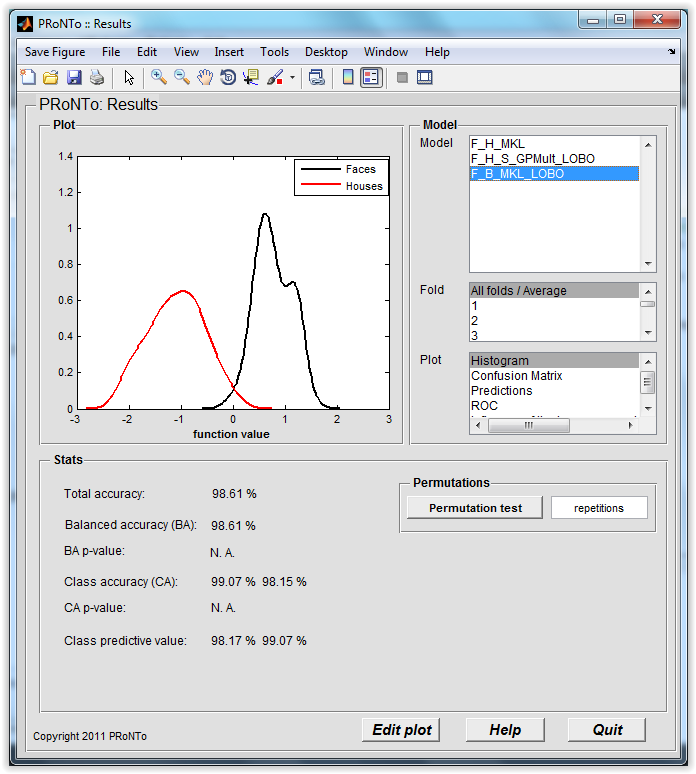
\includegraphics[height=8cm]{images/prt_ui_results_statsTable.png}
\caption{Example statistics for all folds of a two-class problem modelled by an L1-MKL.}
\label{fig_prt_ui_results_statsTable}
\end{center}
\end{figure}

\subsection{Regression}

As previously mentioned, model performance for regression is assessed by the correlation between the predictions and the targets (linear correlation), the coefficient of determination ($R^2$), the mean square error (MSE), and the normalized MSE. An example of such stats window is displayed in Figure \ref{fig_prt_ui_results_statsTableReg}.

\begin{figure}[h!]
\begin{center}
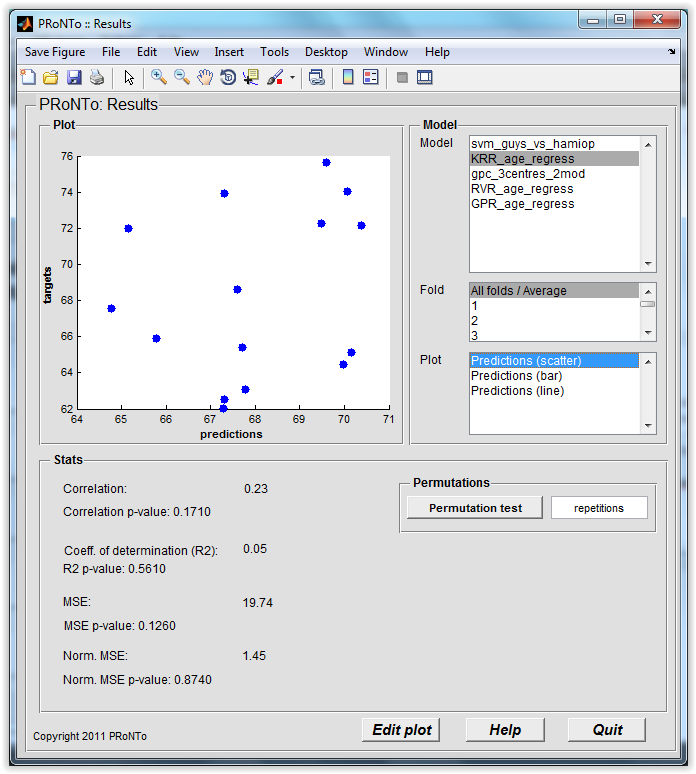
\includegraphics[height=8cm]{images/prt_ui_results_statsTableReg.PNG}
\caption{Example statistics for all folds of a KRR modelling on 15 data points.}
\label{fig_prt_ui_results_statsTableReg}
\end{center}
\end{figure}

% We have the following fields in stats, stats.r2 'Coefficient of Determination', stats.mse 'Mean Squared Error', stats.nmse 'Normalised Mean Squared Error', all calculated in prt_stats.m
The mean-squared error is calculated as:
\begin{equation}
\begin{aligned}
MSE=\frac{1}{N}\sum_{n} (y_n-f(\mathbf{x}_n))^2
\end{aligned}
\end{equation}
This is the standard measure when assessing goodness-of-fit for regression models. 
%There are two important things to remember when using this measure. Firstly, its value is disproportionately affected by bad predictions, because of the 'squared' term. Secondly, its value will be affected by the range of y ie. ....
%Note that the value of this measure is affected by the scale of y. 
%We therefore also calculate 
%the Normalised Mean Square Error, `NMSE':
Since the magnitude of the MSE depends on the scale of $y$, we also calculate the Normalised Mean Square Error, `Norm. MSE':
\begin{equation}
\begin{aligned}
Norm. MSE=\frac{MSE}{(y_{max}-y_{min})}
\end{aligned}
\end{equation}
where we divide the MSE by the range of the targets over the 
%ie., training and test, 
data. This gives a scale invariant measure of prediction accuracy.
In addition, the correlation coefficient of the targets and predictions are determined:
\begin{equation}
\begin{aligned}
CORR=\frac{\sum_{n} (y_n-\mu_y) (f(\boldsymbol{x}_n)-\mu_f)}{\left\{\sum_{n} (y_n-\mu_y)^2 \sum_{n} (f(\boldsymbol{x}_n)-\mu_f)^2\right\}^\frac{1}{2}}
\end{aligned}
\end{equation}
in which $\mu_y$ and $\mu_f$ are the sample means of the targets and predictions respectively. The resulting measure $-1<CORR<1$ provides a measure of the strength of the linear dependence between the targets and the predicted targets, with values close to zero indicating no relationship, values close to 1 indicating a positive relationship, and values close to -1 indicating a negative relationship. Values of $CORR$ less than zero would imply that the model has performed poorly, as this would mean that targets with large values tend to be given smaller predicted values than targets with small values. However, it should be remembered that a large positive value of $CORR$ does not \emph{necessarily} mean that the model is giving accurate predictions, since 
%multiplying all the predictions by a constant scaling factor gives the same value for $CORR$. 
a global scaling and shifting of the predictions gives the same value for $CORR$. 
We would therefore recommend examining both $CORR$ and $MSE$, as well as the scatterplots, to verify that the model is performing well.  For completeness, the statistics table also include the `coefficient of determination' $R^2$, which is given by
\begin{equation}
\begin{aligned}
R^2=CORR^2
\end{aligned}
\end{equation}


\subsection{Permutation testing}

Much of statistical theory and machine learning theory rests on the assumption that the data is
IID (independently and identically distributed). However, in functional neuroimaging this assumption
is often not met, due to e.g. within-run correlations and haemodynamic effects. Therefore, classical estimates of
confidence intervals (such as the binomial confidence interval) may not always
be appropriate. Permutation testing is a non-parametric procedure that allows to obtain meaningful 
confidence intervals and p-values in this case. Because it requires retraining the model a number of times, 
which can be costly in computation time, this is not done by default. After filling in the {\tt repetitions}
field with a number of repetitions $R$, pressing the {\tt Permutation test} button will estimate the model for the specified number of times with permuted labels/targets, and produce a  p-value for performance statistics (see Figure~\ref{fig_prt_ui_results_statsTable}). The smallest increment in p-value is equal to $1/R$ (e.g. 20 permutations gives you increments of 0.05), with a minimum value of $1/R$ (i.e. running 10 permutations will never lead to statistically significant result at the commonly used threshold of $p<0.05$). Usually, we would recommend computing several hundreds to a thousand permutations.

For both classification and regression models, the p-value associated with each performance measure can be estimated using permutations. Until they have been estimated, `N.A.' will be displayed (standing for `not available').

\textbf{Important note:} This step is essential to assess model performance! It is not methodologically sound to simply assume that the chance level is close to $50\%$ and that any balanced accuracy higher than that threshold is significant. Please report p-values as computed from permutations along with model performance.

% XXX Maybe ref Golland TR


% $Id: gui_disres.tex 395 2011-11-17 22:34:59Z cphillip $
%
% Written by J. Schrouff for v2.0
%_______________________________________________


\chapter{Display voxel and region contribution}
\label{chap:DisWeights}
\minitoc

\section{Introduction}

Another important aspect of pattern recognition modelling when applied to neuroimaging is trying to interpret the models' parameters or weights. Some brain 
areas are probably more informative about class membership/regression targets than others. For example, in a visual
task, we would expect discriminative information in the occipital lobe. This can be seen as \textit{information mapping}, and it can be helpful to evaluate a specific model - if
the discriminative weight of a machine is concentrated in the eyes, for example, it is important
to correct the mask used in the analysis to exclude them. In the case of linear kernels, the classifier/regression weight
vector is a linear combination or weighted average of the training examples, and can be plotted
as an image representing a weight map. The \textit{weight map} is therefore a spatial representation
of the decision function, i.e. every voxel within the mask contributes with a certain weight to the decision function. 
Pattern recognition models (classifiers or regression functions) are multivariate, i.e. they
take into account correlations in the data. Since the discrimination or prediction is
based on the whole brain pattern, rather than on individual regions or voxels, all voxels
contribute to the classification or regression and no conclusions should be drawn about a particular
subset of voxels in isolation.

Starting from PRoNTo v2.0, it is possible to derive weights at the region level (as anatomically defined by an atlas, from MKL or from summarizing the weights). This window allows to display maps of voxel and of region contribution. Furthermore, the region contributions can be ranked in descending order, yielding a sorted list of regions according to their contribution to the classification/regression model. We hope this will help the interpretation of model parameters in terms of cognitive neuroscience.

\textbf{Important note:} The implemented version of MKL (\cite{Rakotomamonjy2008}) is sparse in the kernel combination. This means that only a few regions/modalities will contribute to the model. However, this selection of regions/modalities might depend on the dataset, and small variations in the dataset (as induced by cross-validation) might lead to different subsets of regions/modalities begin selected. Therefore, care should be taken when reporting selected regions/modalities and each fold should be looked at separately. We also provide a quantification of the variability across folds of the ranking of the regions/modalities (`Expected Ranking', see further) to provide some insights on this issue.


\section{Displaying weights}

To launch the `Display weights' window, make sure that weight maps have been computed for at least one model (Compute Weights, Chapter~\ref{chap:ComputeWeights}).

In the {\tt Review Options} panel, press {\tt Display weights}. At the `Select PRT.mat' window,
navigate to where your {\tt PRT.mat} file is stored (using the left column), and select it in the
right column. The display window then opens (Figure \ref{fig_prt_ui_weights_empty}).

\begin{figure}[h!]
\begin{center}
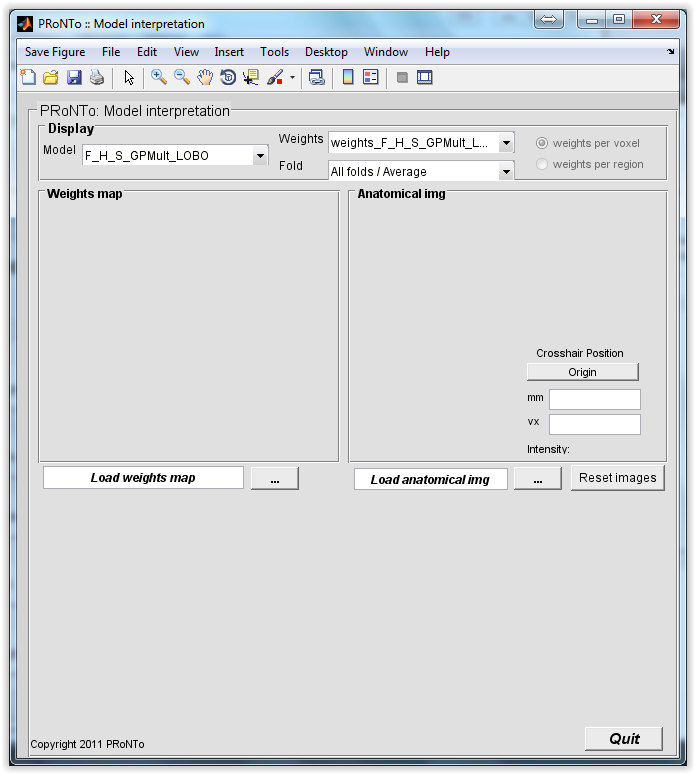
\includegraphics[height=9cm]{images/prt_ui_weights_empty.PNG}
\caption{Display weights main window after selection of PRT.mat.}
\label{fig_prt_ui_weights_empty}
\end{center}
\end{figure}


The window is divided into four panels; going from top left to bottom left, they
are:
\begin{description}
\item[Display]: This panel allows the user to choose which model and image to display, as well as whether to display the voxel weights or the region contributions.
\item[Weights map]: This displays three projections of the selected weight map and allows to navigate it.
\item[Anatomical img]: If an anatomical image has been loaded, this will display three projections,
and the cross-hair will be synchronised with the weight map.
\item[Additional plots]: The blank area at the bottom of the window will display additional information about the model parameters, such as a sorted list of the regions according to their contribution (if weights per region were computed, in the form of a table) and a bar plot of the relative region contribution. If MKL modelling was performed based on multiple modalities, the same table and bar plot will display the relative contributions of each modality to the decision function. 
\end{description}

\subsection{Select image to display}

The \texttt{Display} panel shows the models for which weights were computed and weight images were found in the same folder as the PRT. For each model, the list of images available is displayed in the \texttt{Weights} pop-down list. Typically, one image will be created for a binary comparison or regression with only one modality or multiple modalities concatenated in samples (e.g. multiple runs). On the other hand, multiclass classification models will return one image per class (with the index of the class appended to the name of the image). In the same way, multiple modalities used in multiple kernels will lead to the building of \textit{number of modalities} images. For each image, the weight map can be displayed for each fold or for their average. In PRoNTo v2.0, it is possible to display the contributions of each voxel (\texttt{weights per voxel}) or of each region (\texttt{weights per region}, if previously computed).

\textbf{Note:} the weight images (per voxel and per region) are automatically detected in the list of files in the PRT folder according to the name specified in the `Compute weights' step (Chapter \ref{chap:ComputeWeights}). Modifying the image name afterwards or moving the images might lead to warning messages and the images will not be listed in the GUI.

To display a weight image, select a model, an image and a fold. If only weights per voxel were estimated, the window will look similar to Figure \ref{fig_prt_ui_weights_img}.

\begin{figure}[h!]
\begin{center}
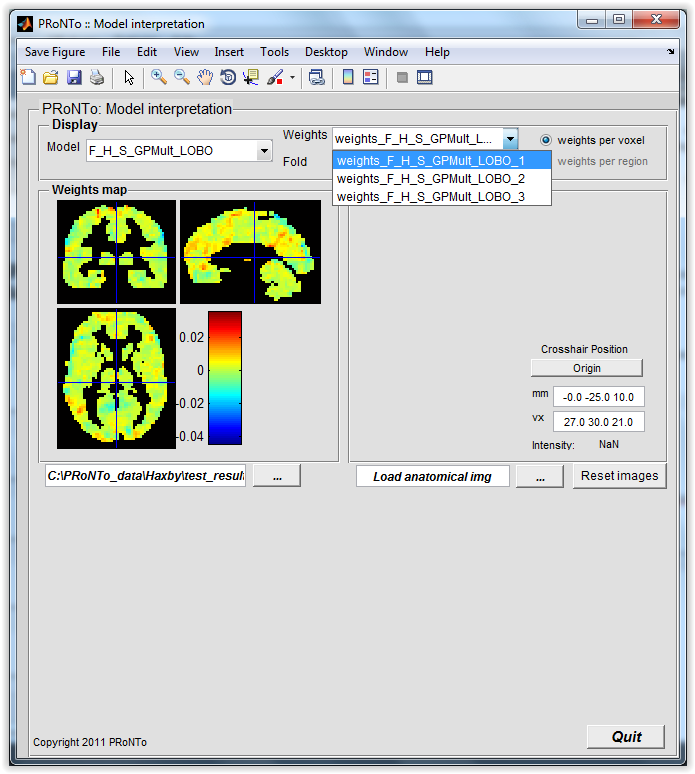
\includegraphics[height=9cm]{images/prt_ui_weights_img.PNG}
\caption{Displaying weight image for class 1 of a three-class GP model (Haxby dataset).}
\label{fig_prt_ui_weights_img}
\end{center}
\end{figure}

\subsection{Weights map}

The weight map is displayed with a cross-hair and a colorbar. The colorbar indicates the
relative importance of the voxel in the decision function. This value is also
indicated in the {\tt intensity} field of the {\tt Anatomical img} panel. Note that all voxels
in the mask contribute to the decision function, since the analysis is multivariate. Contrary
to common practice in Statistical Parametric Mapping, which is a mass-univariate approach, {\em it does
not make sense to isolate part of the pattern and report only on the peaks of the distribution
of the decision function's weight map, unless they have perfectly null contribution (as might happen with sparse models such as L1-MKL modelling)}. 

Below the displayed image, an edit box and a `browse' ($[${\tt ...}$]$) button also allow to load a weight image (.img) that is not linked to a model (e.g. from a previous PRoNTo version).

\subsection{Anatomical image}

By clicking on the $[${\tt ...}$]$ button next to the {\tt Load anatomical img} field, 
a dialogue opens that allows you to select an anatomical images {\tt .img} file that was co-registered with the data images.

In this panel, the cross-hair position is displayed in voxels and in mm. It can also be reset to the origin of the image. For each position, the corresponding voxel weight is displayed in the `intensity' field.

\subsection{Additional plots}

Additional information will be displayed in two main cases:
\begin{itemize}
\item \textbf{Multiple Kernel Learning modelling:} MKL modelling, based on modalities or on regions as defined by an atlas, will provide weights at two levels: the kernel level and the voxel level. The kernel contributions, which sum to 1, can then be ranked in descending order. 
\item \textbf{Summarizing weights per region:} in PRoNTo v2.0, weights can be summarized within regions of interest as defined by an atlas (user-specified). For each region, a normalized contribution can be defined, and those contributions can then be ranked in descending order. 
\end{itemize}

In both cases, the region/modality contributions will be displayed in a table as well as in a bar plot, for each fold and for their average (according to the selected fold in the \texttt{Display} panel). An example is displayed in Figure \ref{fig_prt_ui_weights_ROI}, for weight summarization after GP modelling.

\begin{figure}[h!]
\begin{center}
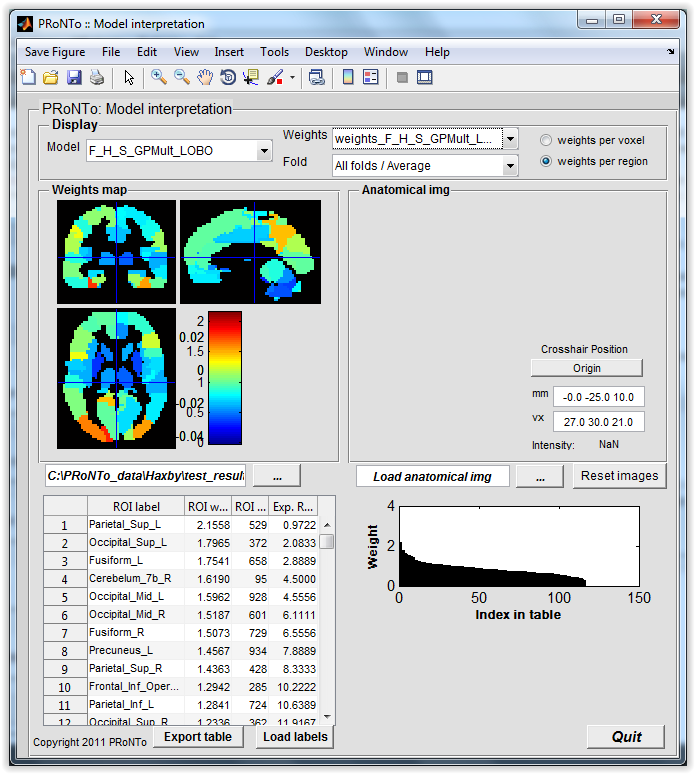
\includegraphics[height=9cm]{images/prt_ui_weights_ROI.PNG}
\caption{Displaying ROI contributions for class 1 of a three-class GP model (Haxby dataset).}
\label{fig_prt_ui_weights_ROI}
\end{center}
\end{figure}

In the case where kernels were built both at the modality and at the region level (i.e. multiple modalities with each multiple regions as defined by an atlas), two tables will be displayed (one for regions, one for modalities). The table for modalities will sum the contributions of each region within that modality.

\subsubsection{Sorted table of region/modality contributions}

The displayed table comprises one row per region and 5 columns (for an example on ROIs, as displayed in Figure \ref{fig_prt_ui_weights_ROI}):

\begin{itemize}
\item \textbf{Index of the ROI:} The first column displays the ranking of the region of interest in the selected fold, according to its contribution.
\item \textbf{ROI Label:} When using the atlas provided in \textit{your PRoNTo folder/atlas}, the labels of each region will be loaded automatically from a .mat, stored alongside the atlas. If using another atlas, the labels can be loaded through the `Load Labels' button. In this case, the user should select a .mat comprising a cell array of size \textit(number of regions,1), with the label for each region in the corresponding cell (in characters). The cell array should be saved under the variable name `ROI\_ names'. Otherwise, generic names will be used (e.g. ROI\_ 1).
\item \textbf{ROI weight:} The (normalized) contribution of each region is displayed in the third column (in \%). The rows of the table are sorted in descending order according to this value. 
\item \textbf{ROI size:} This column displays the size of the ROI in voxels. This gives indications on the overlap between the atlas and the data.
\item \textbf{Expected Ranking}: This measure reflects how stable the ranking of the region is across folds. It is computed from the ranking in each fold (see \cite{Schrouff2013a} for details), and is therefore the same, whether the user is displaying fold 1, or the average of all folds. If the Expected Ranking (ER) is close to the ranking in the selected fold, then it reflects that this region has a similar ranking across folds. On the contrary, if the ER is quite different from the ranking shown for the selected fold, this means that the ranking might be variable across folds. This variability can come from the fact that the region did not have the same contribution to slightly different datasets. It might also happen that it is not selected at all in some folds (as can happen with L1-MKL since it will not select kernels with correlated information).
\end{itemize}

When selecting a specific region label in the table, the weight map will only display colored voxel or region weights (according to which plot was selected) for this region, the rest of the image being in grey scale. This allows e.g. to look closely at the voxel weights within a region that highly contributes to the selected model and fold (Figure \ref{fig_prt_ui_weights_specROI}).

\begin{figure}[h!]
\begin{center}
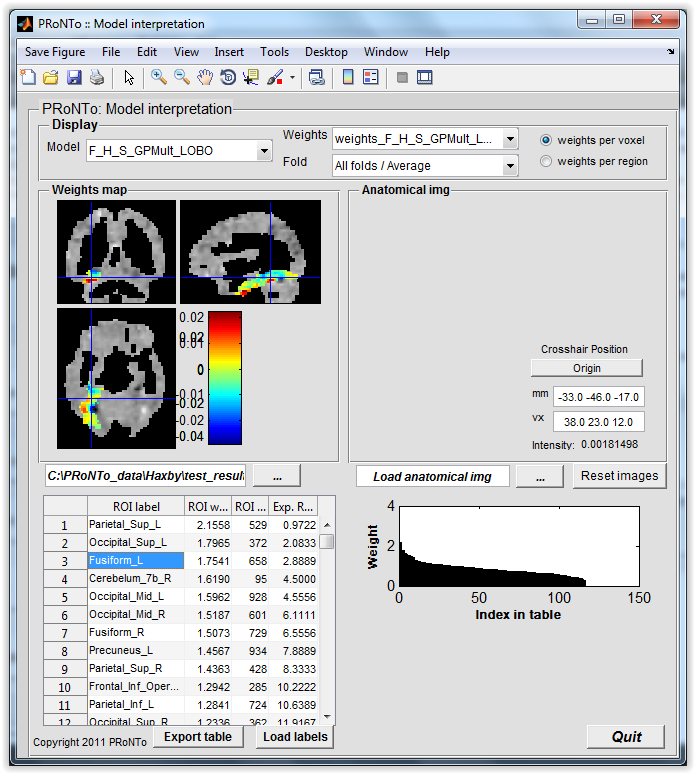
\includegraphics[height=9cm]{images/prt_ui_weights_specROI.PNG}
\caption{Displaying fusiform weights for binary MKL model (Haxby data).}
\label{fig_prt_ui_weights_specROI}
\end{center}
\end{figure}


Finally, the table can be exported as a text file using the `Export Table' button.

\subsubsection{Bar plot of contributions}
The bar plot displays the third column of the table, i.e. the contribution of each ROI or modality to the decision function. The x-axis represents the index of the ROI in the table (i.e. first column of the table), in the selected fold, while the y-axis displays the contribution of each region/modality. The bar graph provides insights on how sparse or dense the region/modality contributions are.






%%%%%% BATCHING HELP %%%%%%
%==========================================
\part{Batch interfaces}
\label{sec:BATCH}
% Help on the batching system
% These files are automatically generated by prt_latex.m from the batch help fields!
% $Id$ 

\chapter{Data \& Design  \label{Chap:data}}

\vskip 1.5cm

Specify the data and design for each group (minimum one group).


\section{Directory}
Select a directory where the PRT.mat file containing the specified design and data matrix will be written.


\section{Groups}
Add data and design for one group. Click 'new' or 'repeat' to add another group.


\subsection{Group}
Specify data and design for the group.


\subsubsection{Name}
Name of the group. Example: 'Controls'.


\subsubsection{Select by}
Depending on the type of data at hand, you may have many images (scans) per subject, such as a fMRI time series, or you may have many subjects with only one or a small number of images (scans) per subject , such as PET images. If you have many scans per subject select the option 'subjects'. If you have one scan for many subjects select the option 'scans'.


\paragraph{Subjects}
Add subjects/scans.


\subparagraph{Subject}
Add new modality for this subject.


\textbf{Modality}
Add new modality.


\textsc{Name}
Name of modality. Example: 'BOLD'. The names should be consistent accross subjects/groups and the same names specified in the masks.


\textsc{Interscan interval}
Specify interscan interval (TR). The units should be seconds.


\textsc{Scans}
Select scans (images) for this modality. They must all have the same image dimensions, orientation, voxel size etc.


\textsc{Data \& Design}
Specify data and design.


\textsl{Load SPM.mat}
Load design from SPM.mat (if you have previously specified the experimental design with SPM).


\textsl{Specify design}
Specify design: scans (data), onsets and durations.


\textit{Units for design}
The onsets of events or blocks can be specified in either scans or seconds.


\textit{Conditions}
Specify conditions. You are allowed to combine both event- and epoch-related responses in the same model and/or regressor. Any number of condition (event or epoch) types can be specified.  Epoch and event-related responses are modeled in exactly the same way by specifying their onsets [in terms of onset times] and their durations.  Events are specified with a duration of 0.  If you enter a single number for the durations it will be assumed that all trials conform to this duration.For factorial designs, one can later associate these experimental conditions with the appropriate levels of experimental factors.


\textit{Condition}
Specify condition: name, onsets and duration.


\textit{Name}
Name of condition (alphanumeric strings only).


\textit{Onsets}
Specify a vector of onset times for this condition type. 


\textit{Durations}
Specify the event durations. Epoch and event-related responses are modeled in exactly the same way but by specifying their different durations.  Events are specified with a duration of 0.  If you enter a single number for the durations it will be assumed that all trials conform to this duration. If you have multiple different durations, then the number must match the number of onset times.


\textit{Multiple conditions}
Select the *.mat file containing details of your multiple experimental conditions. 



If you have multiple conditions then entering the details a condition at a time is very inefficient. This option can be used to load all the required information in one go. You will first need to create a *.mat file containing the relevant information. 



This *.mat file must include the following cell arrays (each 1 x n): names, onsets and durations. eg. names=cell(1,5), onsets=cell(1,5), durations=cell(1,5), then names{2}='SSent-DSpeak', onsets{2}=[3 5 19 222], durations{2}=[0 0 0 0], contain the required details of the second condition. These cell arrays may be made available by your stimulus delivery program, eg. COGENT. The duration vectors can contain a single entry if the durations are identical for all events.



Time and Parametric effects can also be included. For time modulation include a cell array (1 x n) called tmod. It should have a have a single number in each cell. Unused cells may contain either a 0 or be left empty. The number specifies the order of time modulation from 0 = No Time Modulation to 6 = 6th Order Time Modulation. eg. tmod{3} = 1, modulates the 3rd condition by a linear time effect.



For parametric modulation include a structure array, which is up to 1 x n in size, called pmod. n must be less than or equal to the number of cells in the names/onsets/durations cell arrays. The structure array pmod must have the fields: name, param and poly.  Each of these fields is in turn a cell array to allow the inclusion of one or more parametric effects per column of the design. The field name must be a cell array containing strings. The field param is a cell array containing a vector of parameters. Remember each parameter must be the same length as its corresponding onsets vector. The field poly is a cell array (for consistency) with each cell containing a single number specifying the order of the polynomial expansion from 1 to 6.



Note that each condition is assigned its corresponding entry in the structure array (condition 1 parametric modulators are in pmod(1), condition 2 parametric modulators are in pmod(2), etc. Within a condition multiple parametric modulators are accessed via each fields cell arrays. So for condition 1, parametric modulator 1 would be defined in  pmod(1).name{1}, pmod(1).param{1}, and pmod(1).poly{1}. A second parametric modulator for condition 1 would be defined as pmod(1).name{2}, pmod(1).param{2} and pmod(1).poly{2}. If there was also a parametric modulator for condition 2, then remember the first modulator for that condition is in cell array 1: pmod(2).name{1}, pmod(2).param{1}, and pmod(2).poly{1}. If some, but not all conditions are parametrically modulated, then the non-modulated indices in the pmod structure can be left blank. For example, if conditions 1 and 3 but not condition 2 are modulated, then specify pmod(1) and pmod(3). Similarly, if conditions 1 and 2 are modulated but there are 3 conditions overall, it is only necessary for pmod to be a 1 x 2 structure array.



EXAMPLE:

Make an empty pmod structure: 

  pmod = struct('name',{''},'param',{},'poly',{});

Specify one parametric regressor for the first condition: 

  pmod(1).name{1}  = 'regressor1';

  pmod(1).param{1} = [1 2 4 5 6];

  pmod(1).poly{1}  = 1;

Specify 2 parametric regressors for the second condition: 

  pmod(2).name{1}  = 'regressor2-1';

  pmod(2).param{1} = [1 3 5 7]; 

  pmod(2).poly{1}  = 1;

  pmod(2).name{2}  = 'regressor2-2';

  pmod(2).param{2} = [2 4 6 8 10];

  pmod(2).poly{2}  = 1;



The parametric modulator should be mean corrected if appropriate. Unused structure entries should have all fields left empty.


\textsl{No design}
Do not specify design. This option can be used for modalities (e.g. structural scans) that do not have an experimental design.


\paragraph{Scans}
Depending on the type of data at hand, you may have many images (scans) per subject, such as a fMRI time series, or you may have many subjects with only one or a small number of images (scans) per subject, such as PET images. Select this option if you have many subjects per modality to spatially normalise, but there is one or a small number of scans for each subject. This is a faster option with less information to specify than the 'select by subjects' option. Both options create the same 'PRT.mat' but 'select by scans' is optimised for modalities with no design.


\subparagraph{Modality}
Specify modality, such as name and data.


\textbf{Name}
Name of modality. Example: 'BOLD'. The names should be consistent accross subjects/groups and the same names specified in the masks.


\textbf{Files}
Select scans (images) for this modality. They must all have the same image dimensions, orientation, voxel size etc.


\textbf{Regression targets (per scans)}
Enter one regression target per scan. or enter the name of a variable.  This variable should be a vector [Nscans x 1], where Nscans is the number of scans/images.


\textbf{Covariates}
Select a .mat file containing your covariates (i.e. any other data/information you would like to include in your design). This file should contain a variable 'R' with a matrix of covariates. On covariate per image is expected.


\section{Masks}
Select first-level (pre-processing) mask for each modality. The name of the modalities should be the same as the ones entered for subjects/scans.


\subsection{Modality}
Specify name of modality and file for each mask. The name should be consistent with the names chosen for the modalities (subjects/scans).


\subsubsection{Name}
Name of modality. Example: 'BOLD'. The names should be consistent accross subjects/groups and the same names specified in the masks.


\subsubsection{File}
Select one first-level mask (image) for each modality. This mask is used to optimise the prepare data step. In 'specify model' there is an option to enter a second-level mask, which might be used to select only a few areas of the brain for subsequent analyses.


\section{fMRI\_Des}
fMRI design specific parameters, HRF overlap and delay.


\subsection{HRF overlap}
If using fMRI data please specify the width of the hemodynamic response function (HRF). This will be used to calculate the overlap between events. Leave as 0 for other modalities (other than fMRI).


\subsection{HRF delay}
If using fMRI data please specify the delay of the hemodynamic response function (HRF). This will be used to calculate the overlap between events. Leave as 0 for other modalities (other than fMRI).


\section{Review}
Choose 'Yes' if you would like to review your data and design in a separate window.


% $Id$ 

\chapter{Feature set/Kernel  \label{Chap:fs}}

\vskip 1.5cm

Compute feature set according to the design specified


\section{Load PRT.mat}
Select data/design structure file (PRT.mat).


\section{Feature/kernel name}
Target name for kernel matrix. This should containonly alphanumerical characters or underscores (\_).


\section{Modalities}
Add modalities


\subsection{Modality}
Specify modality, such as name and data.


\subsubsection{Modality name}
Name of modality. Example: 'BOLD'. Must match design specification


\subsubsection{Scans / Conditions}
Which task conditions do you want to include in the kernel matrix? Select conditions: select specific conditions from the timeseries. All conditions: include all conditions extracted from the timeseries. All scans: include all scans for each subject. This may be used for modalities with only one scan per subject (e.g. PET), if you want to include all scans from an fMRI timeseries (assumes you have not already detrended the timeseries and extracted task components)


\paragraph{All scans}
No design specified. This option can be used for modalities (e.g. structural scans) that do not have an experimental design or for an fMRI designwhere you want to include all scans in the timeseries


\paragraph{All Conditions}
Include all conditions in this kernel matrix


\subsubsection{Voxels to include}
Specify which voxels from the current modality you would like to include


\paragraph{All voxels}
Use all voxels in the design mask for this modality


\paragraph{Specify mask file}
Select a mask for the selected modality.


\subsubsection{Detrend}
Type of temporal detrending to apply


\paragraph{None}
Do not detrend the data 


\paragraph{Polynomial detrend }
Perform a voxel-wise polynomial detrend on the data (1 is linear detrend) 


\subparagraph{Order}
Enter the order for polynomial detrend (1 is linear detrend)


\paragraph{Discrete cosine transform}
Use a discrete cosine basis set to detrend the data.


\subparagraph{Cutoff of high-pass filter (second)}
The default high-pass filter cutoff is 128 seconds (same as SPM)


\subsubsection{Scale input scans}
Do you want to scale the input scans to have a fixed mean (i.e. grand mean scaling)?


\paragraph{No scaling}
Do not scale the input scans


\paragraph{Specify from *.mat}
Specify a mat file containing the scaling parameters for each modality.


\subsubsection{Use atlas to build ROI specific kernels}
Select an atlas file to build one kernel per ROI. The AAL atlas (named 'aal\_79x91x69.img') is available in the 'atlas' subdirectory of PRoNTo


\section{Use one kernel per modality}
Select "Yes" to use one kernel per modality.


% $Id$ 

\chapter{Specify model  \label{Chap:model}}

\vskip 1.5cm

Construct model according to design specified


\section{Load PRT.mat}
Select data/design structure file (PRT.mat).


\section{Model name}
Name for model


\section{Use kernels}
Are the data for this model in the form of kernels/basis functions? If 'No' is selected, it is assumed the data are in the form of feature matrices


\section{Feature sets}
Enter the name of a feature set to include in this model. This can be kernel or a feature matrix. 


\section{Model Type }
Select which kind of predictive model is to be used.


\subsection{Classification}
Specify classes and machine for classification.


\subsubsection{Classes}
Specify which elements belong to this class. Click 'new' or 'repeat' to add another class.


\paragraph{Class}
Specify which groups, modalities, subjects and conditions should be included in this class


\subparagraph{Name}
Name for this class, e.g. 'controls' 


\subparagraph{Groups}
Add one group to this class. Click 'new' or 'repeat' to add another group.


\textbf{Group}
Specify data and design for the group.


\textsc{Group name}
Name of the group to include. Must exist in PRT.mat


\textsc{Subjects}
Subject numbers to be included in this class. Note that individual numbers (e.g. 1), or a range of numbers (e.g. 3:5) can be entered


\textsc{Conditions / Scans}
Which task conditions do you want to include? Select conditions: select specific conditions from the timeseries. All conditions: include all conditions extracted from the timeseries. All scans: include all scans for each subject. This may be used for modalities with only one scan per subject (e.g. PET), if you want to include all scans from an fMRI timeseries (assumes you have not already detrended the timeseries and extracted task components)


\textsl{Specify Conditions}
Specify the name of conditions to be included 


\textit{Condition}
Specify condition:.


\textit{Name}
Name of condition to include.


\textsl{All Conditions}
Include all conditions in this model


\textsl{All scans}
No design specified. This option can be used for modalities (e.g. structural scans) that do not have an experimental design or for an fMRI designwhere you want to include all scans in the timeseries


\subsubsection{Machine}
Choose a prediction machine for this model


\paragraph{SVM Classification}
Binary support vector machine.


\subparagraph{Optimize hyper-parameter}
Whether to optimize C, the SVM hyper-parameter, or not. If Yes, than provide a range of possible values for C, in the form min:step:max. Examples: 10.\^[-2:5] or 1:100:1000 or 0.01 0.1 1 10 100. If not, a default value will be used (C=1).


\subparagraph{Soft-margin hyper-parameter}
Value(s) for prt\_machine\_svm\_bin: soft-margin C. Examples: 10.\^[-2:5] or 1:100:1000 or 0.01 0.1 1 10 100.


\subparagraph{Cross-validation type for hyper-parameter optimization}
Choose the type of cross-validation to be used


\textbf{Leave one subject out}
Leave a single subject out each cross-validation iteration


\textbf{k-folds CV on subjects}
k-partitioning of subjects at each cross-validation iteration


\textsc{k}
Number of folds/partitions for CV. To create a 50%-50%,choose k as 2. Please note that there can be more partitions than specified when leaving subjects per group out. Also note that leaving more than 50% of the data out is not permitted.


\textbf{Leave one subject per group out}
Leave out a single subject from each group at a time. Appropriate for repeated measures or paired samples designs.


\textbf{k-folds CV on subjects per group}
K-partitioning of subjects from each group at a time. Appropriate for repeated measures or paired samples designs.


\textsc{k}
Number of folds/partitions for CV. To create a 50%-50%,choose k as 2. Please note that there can be more partitions than specified when leaving subjects per group out. Also note that leaving more than 50% of the data out is not permitted.


\textbf{Leave one block out}
Leave out a single block or event from each subject each iteration. Appropriate for single subject designs.


\textbf{k-folds CV on blocks}
k-partitioning on blocks or events from each subject each iteration. Appropriate for single subject designs.


\textsc{k}
Number of folds/partitions for CV. To create a 50%-50%,choose k as 2. Please note that there can be more partitions than specified when leaving subjects per group out. Also note that leaving more than 50% of the data out is not permitted.


\textbf{Leave one run/session out}
Leave out a single run (modality) from each subject each iteration. Appropriate for single subject designs with multiple runs/sessions.


\paragraph{Gaussian Process Classification}
Gaussian Process Classification


\subparagraph{Arguments}
Arguments for prt\_machine\_gpml


\paragraph{Multiclass GPC}
Multiclass GPC


\subparagraph{Arguments}
Arguments for prt\_machine\_gpclap


\paragraph{L1 Multi-Kernel Learning}
Multi-Kernel Learning. Choose only if multiple kernels 

were built during the feature set construction (either multiple modalities or ROIs). 

It is strongly advised to "normalize" the kernels (in "operations").


\subparagraph{Optimize hyper-parameter}
Whether to optimize C, the SVM hyper-parameter, or not. If Yes, than provide a range of possible values for C, in the form min:step:max. Examples: 10.\^[-2:5] or 1:100:1000 or 0.01 0.1 1 10 100. If not, a default value will be used (C=1).


\subparagraph{Arguments}
Arguments for prt\_machine\_sMKL\_cla (same as for SVM)Examples: 10.\^[-2:5] or 1:100:1000 or 0.01 0.1 1 10 100.


\subparagraph{Cross-validation type for hyper-parameter optimization}
Choose the type of cross-validation to be used


\textbf{Leave one subject out}
Leave a single subject out each cross-validation iteration


\textbf{k-folds CV on subjects}
k-partitioning of subjects at each cross-validation iteration


\textsc{k}
Number of folds/partitions for CV. To create a 50%-50%,choose k as 2. Please note that there can be more partitions than specified when leaving subjects per group out. Also note that leaving more than 50% of the data out is not permitted.


\textbf{Leave one subject per group out}
Leave out a single subject from each group at a time. Appropriate for repeated measures or paired samples designs.


\textbf{k-folds CV on subjects per group}
K-partitioning of subjects from each group at a time. Appropriate for repeated measures or paired samples designs.


\textsc{k}
Number of folds/partitions for CV. To create a 50%-50%,choose k as 2. Please note that there can be more partitions than specified when leaving subjects per group out. Also note that leaving more than 50% of the data out is not permitted.


\textbf{Leave one block out}
Leave out a single block or event from each subject each iteration. Appropriate for single subject designs.


\textbf{k-folds CV on blocks}
k-partitioning on blocks or events from each subject each iteration. Appropriate for single subject designs.


\textsc{k}
Number of folds/partitions for CV. To create a 50%-50%,choose k as 2. Please note that there can be more partitions than specified when leaving subjects per group out. Also note that leaving more than 50% of the data out is not permitted.


\textbf{Leave one run/session out}
Leave out a single run (modality) from each subject each iteration. Appropriate for single subject designs with multiple runs/sessions.


\textbf{Custom}
Load a cross-validation matrix comprising a CV variable


\paragraph{Custom machine}
Choose another prediction machine


\subparagraph{Function}
Choose a function that will perform prediction.


\subparagraph{Arguments}
Arguments for prediction machine.


\subsection{Regression}
Add group data and machine for regression.


\subsubsection{Groups}
Add one group to this regression model. Click 'new' or 'repeat' to add another group.


\paragraph{Group}
Specify data and design for the group.


\subparagraph{Group name}
Name of the group to include. Must exist in PRT.mat


\subparagraph{Subjects}
Subject numbers to be included in this class. Note that individual numbers (e.g. 1), or a range of numbers (e.g. 3:5) can be entered


\subsubsection{Machine}
Choose a prediction machine for this model


\paragraph{Kernel Ridge Regression}
Kernel Ridge Regression.


\subparagraph{Optimize hyper-parameter}
Whether to optimize K, the KRR hyper-parameter, or not. If Yes, than provide a range of possible values for K, in the form min:step:max. Examples: 10.\^[-2:5] or 1:100:1000 or 0.01 0.1 1 10 100. If not, a default value will be used.


\subparagraph{Regularization}
Regularization for prt\_machine\_krr. Examples: 10.\^[-2:5] or 1:100:1000 or 0.01 0.1 1 10 100.


\subparagraph{Cross-validation type for hyper-parameter optimization}
Choose the type of cross-validation to be used


\textbf{Leave one subject out}
Leave a single subject out each cross-validation iteration


\textbf{k-folds CV on subjects}
k-partitioning of subjects at each cross-validation iteration


\textsc{k}
Number of folds/partitions for CV. To create a 50%-50%,choose k as 2. Please note that there can be more partitions than specified when leaving subjects per group out. Also note that leaving more than 50% of the data out is not permitted.


\textbf{Leave one subject per group out}
Leave out a single subject from each group at a time. Appropriate for repeated measures or paired samples designs.


\textbf{k-folds CV on subjects per group}
K-partitioning of subjects from each group at a time. Appropriate for repeated measures or paired samples designs.


\textsc{k}
Number of folds/partitions for CV. To create a 50%-50%,choose k as 2. Please note that there can be more partitions than specified when leaving subjects per group out. Also note that leaving more than 50% of the data out is not permitted.


\textbf{Leave one block out}
Leave out a single block or event from each subject each iteration. Appropriate for single subject designs.


\textbf{k-folds CV on blocks}
k-partitioning on blocks or events from each subject each iteration. Appropriate for single subject designs.


\textsc{k}
Number of folds/partitions for CV. To create a 50%-50%,choose k as 2. Please note that there can be more partitions than specified when leaving subjects per group out. Also note that leaving more than 50% of the data out is not permitted.


\textbf{Leave one run/session out}
Leave out a single run (modality) from each subject each iteration. Appropriate for single subject designs with multiple runs/sessions.


\textbf{Custom}
Load a cross-validation matrix comprising a CV variable


\paragraph{Relevance Vector Regression}
Relevance Vector Regression. Tipping, Michael E.; Smola, Alex (2001).

"Sparse Bayesian Learning and the Relevance Vector Machine". Journal of Machine Learning Research 1: 211?244.


\paragraph{Gaussian Process Regression}
Gaussian Process Regression


\subparagraph{Arguments}
Arguments for prt\_machine\_gpr


\paragraph{Multi-Kernel Regression}
Multi-Kernel Regression


\subparagraph{Optimize hyper-parameter}
Whether to optimize C, the MKL hyper-parameter, or not. If Yes, than provide a range of possible values for C, in the form min:step:max. Examples: 10.\^[-2:5] or 1:100:1000 or 0.01 0.1 1 10 100. If not, a default value will be used (C=1).


\subparagraph{Arguments}
Arguments for prt\_machine\_sMKL\_reg


\subparagraph{Cross-validation type for hyper-parameter optimization}
Choose the type of cross-validation to be used


\textbf{Leave one subject out}
Leave a single subject out each cross-validation iteration


\textbf{k-folds CV on subjects}
k-partitioning of subjects at each cross-validation iteration


\textsc{k}
Number of folds/partitions for CV. To create a 50%-50%,choose k as 2. Please note that there can be more partitions than specified when leaving subjects per group out. Also note that leaving more than 50% of the data out is not permitted.


\textbf{Leave one subject per group out}
Leave out a single subject from each group at a time. Appropriate for repeated measures or paired samples designs.


\textbf{k-folds CV on subjects per group}
K-partitioning of subjects from each group at a time. Appropriate for repeated measures or paired samples designs.


\textsc{k}
Number of folds/partitions for CV. To create a 50%-50%,choose k as 2. Please note that there can be more partitions than specified when leaving subjects per group out. Also note that leaving more than 50% of the data out is not permitted.


\textbf{Leave one block out}
Leave out a single block or event from each subject each iteration. Appropriate for single subject designs.


\textbf{k-folds CV on blocks}
k-partitioning on blocks or events from each subject each iteration. Appropriate for single subject designs.


\textsc{k}
Number of folds/partitions for CV. To create a 50%-50%,choose k as 2. Please note that there can be more partitions than specified when leaving subjects per group out. Also note that leaving more than 50% of the data out is not permitted.


\textbf{Leave one run/session out}
Leave out a single run (modality) from each subject each iteration. Appropriate for single subject designs with multiple runs/sessions.


\textbf{Custom}
Load a cross-validation matrix comprising a CV variable


\paragraph{Custom machine}
Choose another prediction machine


\subparagraph{Function}
Choose a function that will perform prediction.


\subparagraph{Arguments}
Arguments for prediction machine.


\section{Cross-validation type}
Choose the type of cross-validation to be used


\subsection{Leave one subject out}
Leave a single subject out each cross-validation iteration


\subsection{k-folds CV on subjects}
k-partitioning of subjects at each cross-validation iteration


\subsubsection{k}
Number of folds/partitions for CV. To create a 50%-50%,choose k as 2. Please note that there can be more partitions than specified when leaving subjects per group out. Also note that leaving more than 50% of the data out is not permitted.


\subsection{Leave one subject per group out}
Leave out a single subject from each group at a time. Appropriate for repeated measures or paired samples designs.


\subsection{k-folds CV on subjects per group}
K-partitioning of subjects from each group at a time. Appropriate for repeated measures or paired samples designs.


\subsubsection{k}
Number of folds/partitions for CV. To create a 50%-50%,choose k as 2. Please note that there can be more partitions than specified when leaving subjects per group out. Also note that leaving more than 50% of the data out is not permitted.


\subsection{Leave one block out}
Leave out a single block or event from each subject each iteration. Appropriate for single subject designs.


\subsection{k-folds CV on blocks}
k-partitioning on blocks or events from each subject each iteration. Appropriate for single subject designs.


\subsubsection{k}
Number of folds/partitions for CV. To create a 50%-50%,choose k as 2. Please note that there can be more partitions than specified when leaving subjects per group out. Also note that leaving more than 50% of the data out is not permitted.


\subsection{Leave one run/session out}
Leave out a single run (modality) from each subject each iteration. Appropriate for single subject designs with multiple runs/sessions.


\subsection{Custom}
Load a cross-validation matrix comprising a CV variable


\section{Include all scans}
This option can be used to pass all the scans for each subject to the learning machine, regardless of whether they are directly involved in the classification or regression problem. For example, this can be used to estimate a GLM from the whole timeseries for each subject prior to prediction. This would allow the resulting regression coefficient images to be used as samples.


\section{Data operations}
Specify operations to apply


\subsection{Mean centre features}
Select an operation to apply.


\subsection{Other Operations}
Include other operations?


\subsubsection{No operations}
No design specified. This option can be used for modalities (e.g. structural scans) that do not have an experimental design or for an fMRI designwhere you want to include all scans in the timeseries


\subsubsection{Select Operations}
Add zero or more operations to be applied to the data before the prediction machine is called. These are executed within the cross-validation loop (i.e. they respect training/test independence) and will be executed in the order specified. 


\paragraph{Operation}
Select an operation to apply.


% $Id$ 

\chapter{Run model  \label{Chap:cv_model}}

\vskip 1.5cm

Trains and tests the predictive machine using the cross-validation structure specified by the model.


\section{Load PRT.mat}
Select PRT.mat (file containing data/design structure).


\section{Model name}
Name of a model. Must match your entry in the 

'Specify model' batch module.


\section{Do permutation test?}
Perform a permutation test on accuracy, or not


\subsection{No permutation test}
Do not perform permutation test


\subsection{Permutation test}
Perform a permutation test.


\subsubsection{Number of permutations}
Enter the number of permutations to perform


\subsubsection{Save permutations parameters}
Set to Yes to save the parameterss obtained from eachpermutation.




%%%%%% DATA EXAMPLE %%%%%%
%==========================================
% Help on the data examples
\part{Data processing examples}
% $Id$

\chapter{Block design fMRI dataset}
\label{sec:Block_design_fMRI_dataset}
\minitoc

This chapter will describe the steps necessary to perform a classification using PRoNTo. The dataset\footnote{Pre-processed (realigned and normalised) data from participant 1.} used in this chapter can be found in PRoNTo's website \url{http://www.mlnl.cs.ucl.ac.uk/pronto/prtdata.html} (data set 1) and the whole\footnote{Not pre-processed.} dataset is available in \url{http://data.pymvpa.org/datasets/haxby2001/}.

This fMRI dataset originates from a study on face and object representation in human ventral temporal cortex \cite{Haxby2001}. In this study, the subject was shown a set of grey scale images of 8 categories (faces, houses, cats, chairs, bottles, scissors, shoes and scrambled pictures), with 12 runs/blocks. Each image was displayed for 500 ms and was followed by a 1500 ms rest interval. This experiment consisted on a block-design of 9 scans of task followed by 6 scans of inter-stimulus interval. Images were acquired with a TR of 2.5 s. The full-brain fMRI data was made up by 1452 volumes with 40 x 64 x 64 voxels, each of which with dimensions of 3.5 x 3.75 x 3.75 mm.

For simplicity, in this example we will use PRoNTo to predict if the subject is viewing an image of a Face or a House based on the fMRI scans. We will classify the whole brain images using Support Vector Machines, and a leave one block out cross-validation scheme.

\section{GUI analysis}

We will first analyse the data using PRoNTo's GUI and then repeat the analysis using the {\tt matlabbatch} system.

To start, create a new directory in which to save the results of the analysis, then start up MATLAB and type `prt' or `pronto' in the MATLAB prompt. This will open the main interface of PRoNTo (Figure \ref{fig:mainInterface}).

\begin{figure}[!h]
	\centering
		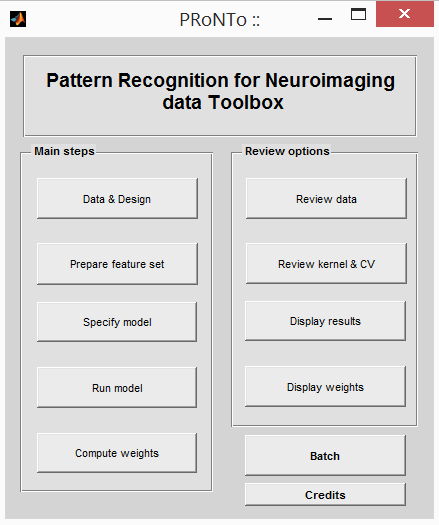
\includegraphics[scale=0.8]{images/Tutorial/classification/mainInterface.png}
	\caption{Main interface of PRoNTo.}
	\label{fig:mainInterface}
\end{figure}

%--------------------------------------------------------------------------
\subsection{Data \& Design}

\begin{itemize}
	
	\item In PRoNTo's main window, click on `Data \& Design' and a new window will open, `Data and design' (Figure \ref{fig:dataDesign}). Then, browse the directory in which to save the PRT structure (saved as `PRT.mat');
	
\begin{figure}[!h]
	\centering
			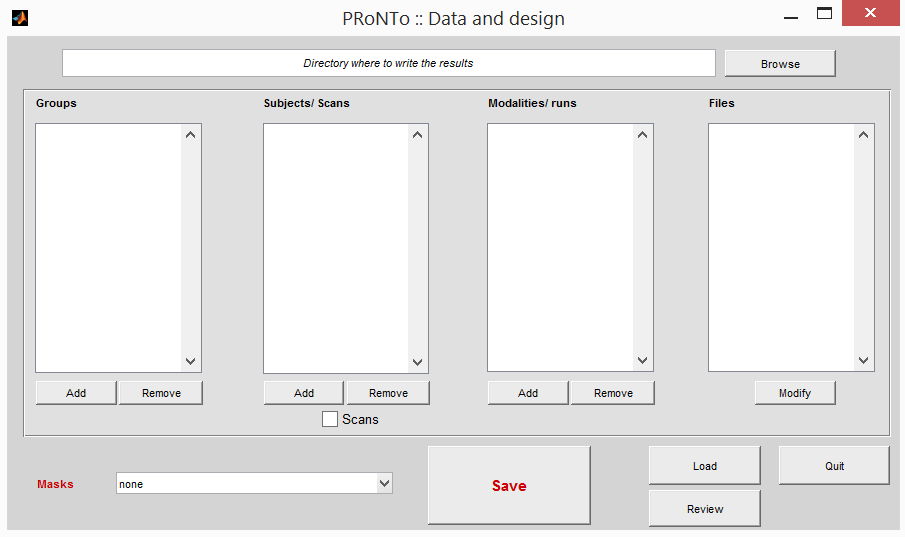
\includegraphics[scale=0.7]{images/Tutorial/classification/dataDesign.png}
	\caption{`Data and design' GUI.}
	\label{fig:dataDesign}
\end{figure}
	
	\item In the panel `Groups', click on `Add' and provide a name to the group (we only have one group/subject), with no spaces, e.g. `G1';
	
	\item Add a subject in the `Subject/Scans' option, e.g. `s1', and leave the `Scans' tick box below the panel unchecked. See Chapter \ref{chap:DataDesign} of the manual for more information on this option;
	
	\item In the `Modalities' panel, click on `Add' and provide a name to the modality, e.g. `fMRI'. In the `Design' field, choose the option `Load SPM.mat' (Figure \ref{fig:modality}). This file is available with the Haxby dataset on PRoNTo's website\footnote{http://www.mlnl.cs.ucl.ac.uk/pronto/prtdata.html} inside the folder Haxby\_dataset/design/;
	
\begin{figure}[!h]
	\centering
		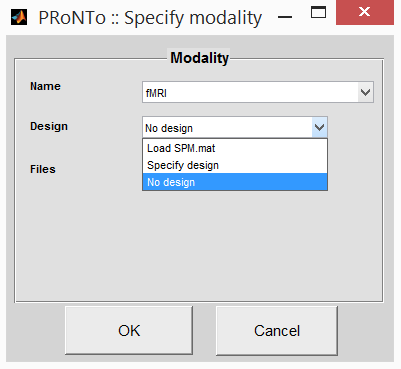
\includegraphics[scale=0.7]{images/Tutorial/classification/modality.png}
	\caption{`Specify modality' GUI allows one to load a specified design from an `SPM.mat' file.}
	\label{fig:modality}
\end{figure}

	\begin{itemize}
	
		\item In case there is no `SPM.mat' file available to use, create a new design by selecting the option `Specify design'. Choose how many conditions you have, which in this case are 8 conditions (corresponding to the 8 categories of images). This will open another window that allows the user to write the names, onsets and durations (if the duration is the same for all events only one value is required) of each condition (Figure \ref{fig:specifyDesign}). The unit in which the onsets/durations are read in this case is `scans' and the interscan interval (TR) is 2.5 seconds. The design information (names, onsets and durations) can be found inside the `Haxby\_design.pdf' file in the Haxby dataset folder. 
	
	\end{itemize}
	
\begin{figure}[!h]
	\centering
		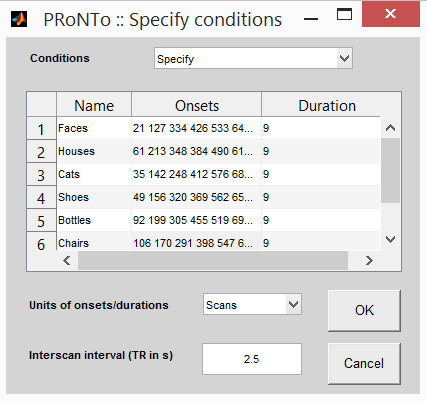
\includegraphics[scale=0.7]{images/Tutorial/classification/specifyDesign.png}
	\caption{`Specify design' GUI to enter the conditions, the units of design, TR and covariates.}
	\label{fig:specifyDesign}
\end{figure}
	
	\item Finally, load all the image files available in the fMRI directory (Haxby\_dataset/fMRI/). You can select all the files by using the right mouse button and clicking on the option `Select All' (Figure \ref{fig:files}). When all the images are selected, click on the `Done' button;
	
		
\begin{figure}[!h]
	\centering
		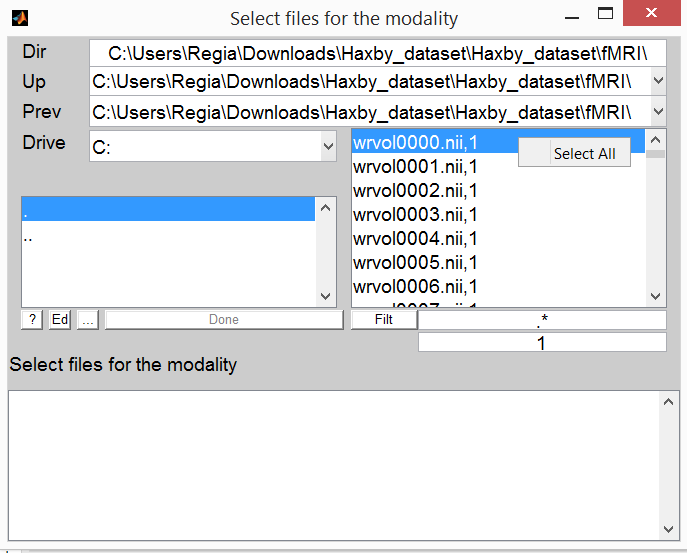
\includegraphics[scale=0.65]{images/Tutorial/classification/files.png}
	\caption{`Files' field is used to select the scans/images for the selected subject.}
	\label{fig:files}
\end{figure}
	
	\item In the `Masks' field, on the bottom left of the `Data and design' window, select the `whole\_brain' mask for the modality specified (Figure \ref{fig:mask}). The mask is available in the masks directory inside the folder Haxby\_dataset/masks/;

\begin{figure}[!h]
	\centering
		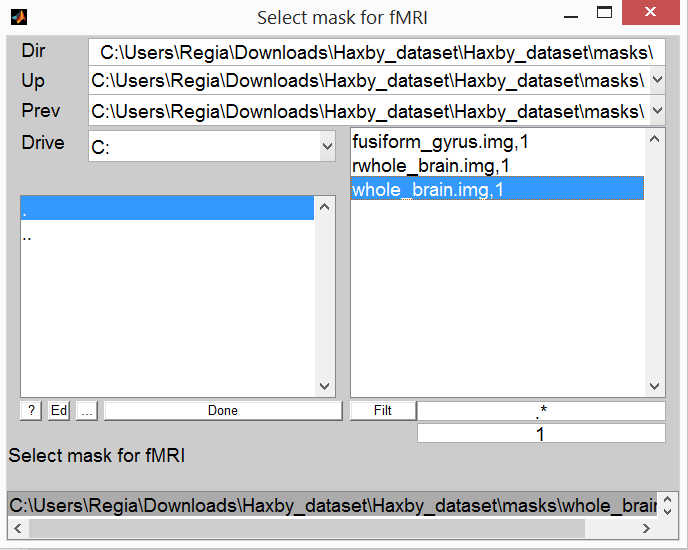
\includegraphics[scale=0.65]{images/Tutorial/classification/mask.png}
	\caption{This window is called when one clicks `Masks'.}
	\label{fig:mask}
\end{figure}

	\item Click on `Review' button to check the data and the design inserted in this modality (Figure \ref{fig:review}). For more information on what one can do with the Review option please see Chapter \ref{chap:DataDesign};
	
	
\begin{figure}[!h]
	\centering
		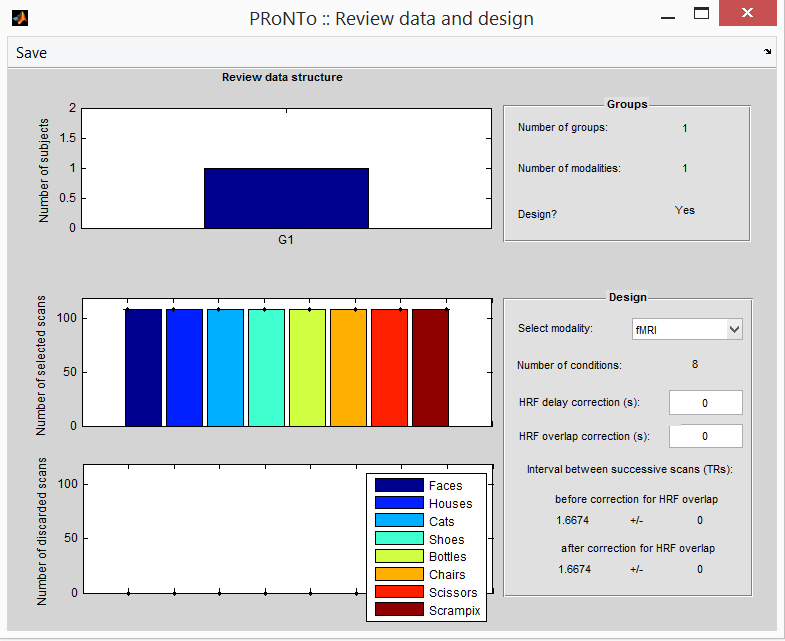
\includegraphics[scale=0.7]{images/Tutorial/classification/review.png}
	\caption{`Review' GUI allows the user to check the data and design.}
	\label{fig:review}
\end{figure}	
	
	\item The `Data and design' window should look similar to the Figure \ref{fig:finalDesign}. Click on `Save' button to create `PRT.mat' file with the structure containing the information that has been previously specified. If no errors are shown in the MATLAB command window, leave the `Data and design' window by clicking `Quit'.
	

\begin{figure}[!h]
	\centering
		\includegraphics[scale=0.7]{images/Tutorial/classification/finalDesign.png}
	\caption{`Data and design' GUI final configuration.}
	\label{fig:finalDesign}
\end{figure}	

\end{itemize}

%--------------------------------------------------------

\subsection{Prepare feature set}

\begin{itemize}
	
	\item In PRoNTo's main window, click on `Prepare feature set' and a new window will open, `Prepare feature set' (Figure \ref{fig:prepareFeature});
	
	\begin{figure}[!h]
	\centering
		\includegraphics[scale=0.7]{images/Tutorial/classification/prepareFeature.png}
	\caption{`Prepare feature set' GUI.}
	\label{fig:prepareFeature}
\end{figure}
	
	\item Select the `PRT.mat' file previously created in the `Data \& Design' step and another window will open, `Specify modality to include' (Figure \ref{fig:specifyModality}), to set the specification of different parameters and options for each modality, which are: 
	
	\begin{itemize}
		\item `Modality' field: select the modality previously specified in the `Data \& Design' step, `fMRI';
		\item `Conditions' field: select `All scans'; 
		\item Parameters box: select the polynomial detrend with order 1 and the 'No scaling' option;
		\item Features box: leave the additional mask field as it is and the `build one kernel per region' tick box unchecked. Then, click on the `Done' button.  
		
			\begin{itemize}
			\item As an optional step, in the `Additional mask for selected modality' field, the user can specify a `second-level' mask, which can be used to select regions of interest (ROIs) on which the classification can be performed. For instance, we can enter the `fusiform\_gyrus' mask available with this dataset; 
			\end{itemize}	
			
			\begin{figure}[!h]
	\centering
		\includegraphics[scale=0.75]{images/Tutorial/classification/specifyModality.png}
	\caption{`Specify modality to include' GUI.}
	\label{fig:specifyModality}
\end{figure}				
		
	\end{itemize}		
		
	\item In the `Prepare feature set' window, provide a name for the feature set, e.g. `HaxbyFeatures';

	\item Click on `Build kernel/data matrix' to build the feature set and kernel (Figure \ref{fig:buildKernel}). It takes a few minutes.


\begin{figure}[!h]
	\centering
		\includegraphics[scale=0.65]{images/Tutorial/classification/buildKernel.png}
	\caption{Preparing feature set.}
	\label{fig:buildKernel}
\end{figure}


\end{itemize}



%---------------------------------------------------------------------

\subsection{Specify model}

\begin{itemize}
	
	\item In PRoNTo's main window, click on `Specify model' and a new window will open, `Specify model' (Figure \ref{fig:specifyModel});
	
	\begin{figure}[!h]
	\centering
		\includegraphics[scale=0.7]{images/Tutorial/classification/specifyModel.png}
	\caption{`Specify Model' GUI.}
	\label{fig:specifyModel}
\end{figure}
	
	\item Select the `PRT.mat' file and provide a name to the model, e.g. `svmFacesHouses';

	\item Select one of the `Feature Set' previously defined. In this case, there is only one `HaxbyFeatures';

	\item	Leave the option `Use kernels' tick box as it is, i.e. `Yes';

	\item	Select the `Classification' model type and click on `Define classes` button. A new window will open, `Specify classes' (Figure \ref{fig:specifyClasses}), to define the number of classes and a name for each class. We will define 2 classes. For `Class 1' select subject `S1' and the condition `Faces' and, similarly, for `Class 2' select subject `S1' and the condition `Houses'. Click on `Done';
	
\begin{figure}[!h]
	\centering
		\includegraphics[height=9cm]{images/Tutorial/classification/specifyClasses.png}
	\caption{`Specify classes' GUI.}
	\label{fig:specifyClasses}
\end{figure}
	
	\item Select the `Binary support vector machine' option, in the `Machine' field;
	
	\item Leave the option `Optimize hyper-parameter' tick box unchecked and `Cross-Validation Scheme' (internal loop) as it is; 
	
	\item Select the `Leave One Block Out' cross-validation scheme (external loop);
	
	\item In the `Data operations' box, select the `Sample averaging (within block)' option, which corresponds to a temporal compression of the data within each block, and `Mean centre features using training data' option. Then, the `Specify model' window should look similar to Figure \ref{fig:finalModel};
	
	\begin{figure}[h!]
	\centering
		\includegraphics[scale=0.7]{images/Tutorial/classification/finalModel.png}
	\caption{`Specify model' GUI final configuration.}
	\label{fig:finalModel}
\end{figure}
	
	\item Click on `Specify and run model' and the model will be immediately estimated, therefore there is no need to use the `Run model' module in this case;

	\item If you do not wish to average the scans within each block (i.e. to do temporal compression), go back to the `Specify model' window, give another name to the model and select the same options mentioned above, except in the data operations part. Here, choose only the `Mean centre features using training data' option. Finish by clicking on the `Specify and run model' button.
\end{itemize}

%--------------------------------------------------------------------

\subsection{Display model (optional step)}

\begin{itemize}
\item To review the model specification, in the main PRoNTo GUI, click on `Review kernel \& CV' and a new window will open, `Review Model Specification' (Figure \ref{fig:reviewModel});

\begin{figure}[h!]
	\centering
		\includegraphics[scale=0.7]{images/Tutorial/classification/reviewModel.png}
	\caption{Review CV \& kernel window.}
	\label{fig:reviewModel}
\end{figure}

\item Select the model, `svmFacesHouses', from the list at the top and click on `Review model'; then, select one class from the list of `Class' to see which groups, subjects and conditions this class comprises (Figure \ref{fig:reviewModelClass});



\begin{figure}[h!]
	\centering
		\includegraphics[scale=0.7]{images/Tutorial/classification/reviewModelClass.png}
	\caption{Review model specification window to Class 1.}
	\label{fig:reviewModelClass}
\end{figure}

\item To review the data and cross-validation matrix click on `Review CV' (Figure \ref{fig:reviewCV}). For more information on what these matrices mean, please consult the previous chapters of the manual;

\begin{figure}[h!]
	\centering
		\includegraphics[scale=0.7]{images/Tutorial/classification/reviewCV.png}
	\caption{Data and cross-validation matrix from `Review CV' option.}
	\label{fig:reviewCV}
\end{figure}

\item To review the kernel, click on `Show kernel' (Figure \ref{fig:reviewKernel}).

\begin{figure}[h!]
	\centering
		\includegraphics[scale=0.7]{images/Tutorial/classification/reviewKernel.png}
	\caption{Kernel matrix used for classification.}
	\label{fig:reviewKernel}
\end{figure}

\end{itemize}

%----------------------------------------------------

\subsection{Compute weights (optional step)}

\begin{itemize}
\item In PRoNTo's main window, click on `Compute weights' and a new window will open, `Compute weights' (Figure \ref{fig:computeWeights});

\begin{figure}[h!]
	\centering
		\includegraphics[scale=0.7]{images/Tutorial/classification/computeWeights.png}
	\caption{`Compute weights' GUI.}
	\label{fig:computeWeights}
\end{figure}

\item Select the `PRT.mat' file;

\item Select the model from the list to `Models computed in PRT', `svmFacesHouses' model;

\item Leave the option `Compute average/kernel weight per region' tick box unchecked;

\item Click on `Compute weights' button. Computations will be displayed on the MATLAB command window.

\end{itemize}

%------------------------------------------------------------------

\subsection{Display results}
\label{display_results}

\begin{itemize}
	
	\item In PRoNTo's main window, click on `Display results' and select the `PRT.mat' file. This will open the main results window (Figure \ref{fig:results});
	
\begin{figure}[h!]
	\centering
		\includegraphics[scale=0.6]{images/Tutorial/classification/results.png}
	\caption{`Results' GUI.}
	\label{fig:results}
\end{figure}
	
	
	\item In the `Model' panel, select the model that you want to view, `svmFacesHouses'. The performance should be similar to the one in Figure \ref{fig:stats};
	
	\begin{figure}[h!]
	\centering
		\includegraphics[scale=0.75]{images/Tutorial/classification/stats.png}
	\caption{Summary for model's performance.}
	\label{fig:stats}
\end{figure}
	
	\item In the `Results' window, one can select a different plot in the `Plots' list;
	
	
	\item Finally, to check the significance of the results, run a permutation test by clicking on `Permutation test' button with 100 repetitions. Results will be displayed on the MATLAB prompt (Figure \ref{fig:permutations}). Please note that 100 repetitions is a small amount, if possible, this should be greater (e.g. 1000).

\begin{figure}[h!]
	\centering
		\includegraphics[height=9cm]{images/Tutorial/classification/permutations.png}
	\caption{Sample of the MATLAB window after the permutation test (100 repetitions).}
	\label{fig:permutations}
\end{figure}

\end{itemize}
	
%------------------------------------------------------------------

\subsection{Display weights}

\begin{itemize}
	
	\item In PRoNTo's main window, click on `Display weights' and select the `PRT.mat' file. This will open the `Model interpretation' window (Figure \ref{fig:modelInterpretationMain});
	
	\begin{figure}[h!]
	\centering
		\includegraphics[scale=0.6]{images/Tutorial/classification/modelInterpretationMain.png}
	\caption{`Model interpretation' GUI.}
	\label{fig:modelInterpretationMain}
\end{figure}

	
	\item By clicking on `Model', svmFacesHouses, an image will appear in the `Weights map' box; and to show the `Anatomical img' you have to load an anatomical image for reference. A template image can be found in SPM's canonical folder (`single\_subj\_T1` file). The final window will look similar to the one shown in the Figure \ref{fig:modelInterpretation}.

\begin{figure}[h!]
	\centering
		\includegraphics[height=10cm]{images/Tutorial/classification/modelInterpretation.png}
	\caption{`Model interpretation' GUI with results.}
	\label{fig:modelInterpretation}
\end{figure}
	
\end{itemize}

%=====================================================



%=====================================================

\section{Batch analysis}
\label{sec:Batch_analysis_svm}

This tutorial will now show how to analyse the same data but using the {\tt matlabbatch} system.

Once again, create a new directory where you wish to save the results. On the main interface of PRoNTo click on the `Batch' button to open the `{\tt matlabbatch}'. Alternatively, type `prt\_batch' on the MATLAB command window. On the menu bar of the batch, there is a PRoNTo menu with the 5 options shown in the main steps interface (Figure \ref{fig:batch}).

\begin{figure}[h!]
	\centering
		\includegraphics[scale=0.6]{images/Tutorial/classification/batch.png}
	\caption{Menu PRoNTo in the main {\tt matlabbatch} window.}
	\label{fig:batch}
\end{figure}

%--------------------------------------------------------------

\subsection{Data \& Design}

\begin{itemize}

	\item Click on `Data \& Design' in the PRoNTo menu (Figure \ref{fig:batchData});
	
	\begin{figure}[h!]
	
	\centering
		\includegraphics[scale=0.6]{images/Tutorial/classification/batchData.png}
	\caption{Data and design module in {\tt matlabbatch}. }
	\label{fig:batchData}
	
	\end{figure}

	\item In the `Directory' field, select a directory where the `PRT.mat' file will be saved. There are three ways of editing all fields in {\tt matlabbatch}: (i) by using the right mouse button and clicking on the current option, (ii) clicking on current button in the window or (iii) by double clicking;
	
	\item In the `Groups' field:
 	
		\begin{itemize}
		
		\item Add one group;
		
		\item In the field `Name', provide a name without spaces to that group, e.g. `G1'; 
		
		\item In the field `Select by', select the `Subjects' option and add one subject;
		
		\item Add one modality for this subject and provide a name, e.g. `fMRI'; define the interscan interval of 2.5 seconds; and in the field `Scans', select all the image files available in the fMRI directory of the Haxby dataset;	
		
		\item In the `Data \& Design' field, choose `Load SPM.mat' option. This file is available with the Haxby dataset on PRoNTo's website\footnote{http://www.mlnl.cs.ucl.ac.uk/pronto/prtdata.html} inside the folder Haxby\_dataset/design/. The batch editor should look similar to the one in Figure \ref{fig:batchGroups};	
		
		\begin{figure}[h!]
	\centering
		\includegraphics[scale=0.6]{images/Tutorial/classification/batchGroups.png}
	\caption{Data and design module in {\tt matlabbatch}. }
	\label{fig:batchGroups}
	\end{figure}
				
		
		\begin{itemize}
	
			\item In case there is no `SPM.mat' file available to use, create a new	design by selecting the option `Specify design'. Choose how many conditions you have, which in this case are 8 conditions (corresponding to the 8 categories of images). The unit in which the onsets/durations are read is `Scans'. Write the names, onsets and durations of each condition (Figure \ref{fig:batchSpecifyDesign});
	
\begin{figure}[h!]
	\centering
		\includegraphics[scale=0.6]{images/Tutorial/classification/batchSpecifyDesign.png}
	\caption{Data and design module. The `Specify design' option.}
	\label{fig:batchSpecifyDesign}
\end{figure}
	
	\end{itemize}

		\end{itemize}
	
	\item In the `Masks' field, add a new modality and provide the same modality name, `fMRI'; and select the `whole\_brain' mask available in the masks directory of the Haxby dataset. The name of the modality here has to be exactly the same as in `Modalities', otherwise it will not work;
	
	%checar aqui
	
	\item Leave the `HRF overlap' and the `HRF delay' fields as default;
	
	\item In the `Review' field, select `Yes' if you would like to review your data and design in a separate window. Otherwise, leave as it is, i.e. `No'.


\end{itemize}

%------------------------------------------------------------

\subsection{Feature set / Kernel}

\begin{itemize}
	\item Click on `Feature set / Kernel' option on PRoNTo's {\tt matlabbatch} menu (Figure \ref{fig:batchFeature});
	
	\begin{figure}[h!]
	\centering
		\includegraphics[scale=0.6]{images/Tutorial/classification/batchFeature.png}
	\caption{Feature set/Kernel module in {\tt matlabbatch}. }
	\label{fig:batchFeature}
\end{figure}
	
	\item With `Load PRT.mat' field selected, click on the `Dependency' button to associate the `PRT.mat' file created in the previous `Data \& Design' step (Figure \ref{fig:batchDependency}) or click on the `Select files' button to browse where `PRT.mat' file was saved;
	
	 	
\begin{figure}[h!]
	\centering
		\includegraphics[scale=0.6]{images/Tutorial/classification/batchDependency.png}
	\caption{Feature set / Kernel module in {\tt matlabbatch}. This window is called to establish a dependency connection with the previous `Data and design' module.}
	\label{fig:batchDependency}
\end{figure}
	
	\item Provide a name to the `Feature/kernel' set, e.g. `HaxbyFeatures';
	
	\item Add one modality and select the modality name with the `Dependency' button\footnote{Or type it in manually, `fMRI', but the name needs to be {\it exactly} the same as the one specified in the `Data \& Design' module.}(Data \& Design:Mod\#1 name);
	
		\begin{itemize}
	
	\item In the `Scans/Conditions' field , select the `All scans' option;
	
	\item In the `Voxels to include' field, select `All voxels' option, this means we are not entering an additional second-level mask;
	
			\begin{itemize}
			\item This is an optional step. In the `Voxels to include' options, the user can specify a `second-level' mask, which would define regions of interest (ROIs) on which the classification can be performed. In this case, select the `fusiform\_gyrus' mask;
			\end{itemize}
	
	\item In the `Detrend' field, select `Polynomial detrend' option with order 1;
	
	\item In the `Scale input scans' field, select `No scaling' option;
	
	\item Leave `Load Atlas' as default. After all these steps, the batch editor should look similar to the one in Figure \ref{fig:batchModality};
	
	\begin{figure}[h!]
	\centering
		\includegraphics[scale=0.6]{images/Tutorial/classification/batchModality.png}
	\caption{Feature set / Kernel module. Selected parameters in the Modality option.}
	\label{fig:batchModality}
\end{figure}
	
	\end{itemize}
	
	\item Leave the `Generate Multiple Kernels' and the `Use one kernel per modality' fields as default.
	

\end{itemize}

%--------------------------------------------------------

\subsection{Specify model}

\begin{itemize}

\item Click on `Specify model' option on PRoNTo's {\tt matlabbatch} menu (Figure \ref{fig:batchSpecifyModel});
	
	\begin{figure}[h!]
	\centering
		\includegraphics[scale=0.6]{images/Tutorial/classification/batchSpecifyModel.png}
	\caption{Specify model module in {\tt matlabbatch}.}
	\label{fig:batchSpecifyModel}
\end{figure}
	
	\item With `Load PRT.mat' field selected, click on `Dependency' button to associate the `PRT.mat' file created in the previous `Feature set / Kernel' step (Figure \ref{fig:batchDependency2}) or click on `Select files' button to browse where `PRT.mat' file was saved;
	
\begin{figure}[h!]
	\centering
		\includegraphics[scale=0.6]{images/Tutorial/classification/batchDependency2.png}
	\caption{Specify model module in {\tt matlabbatch}. This window is called to establish a dependency connection with the previous `Feature set / Kernel' module.}
	\label{fig:batchDependency2}
\end{figure}

	\item Provide a name to the model, e.g. `svmFacesHouses'; 
	
	\item Leave the `Use kernels' field as it is, i.e. `Yes';
	
	\item In the `Feature sets' field, select the feature set name with the `Dependency' button\footnote{or write it {\it exactly} as previously defined in the `Feature set / Kernel' module (option `Feature set/Kernel: Feature/kernel name'), here `HaxbyFeatures'.};
	
	\item Select the `Classification' model type:
	
		\begin{itemize}
		
		\item Add 2 new classes;
		
		\item For Class (1) write `Faces' on the name field and add one group. Select the group name from the `Data \& Design' module (`Data \& Design:Group\#1 name') with the `Dependency' button\footnote{Or write it {\it exactly}, as previously defined in the Data \& Design' module, here `G1'}. Similarly, for Class (2) write `Houses' on the name field and add the group created in the `Data \& Design' module, `G1';	
		
		\item In the `Subjects' field, type `1' (only subject 1 is selected);
		
		\item In the `Conditions / Scans' field, select the `Specify Conditions' option and add a new condition. Provide a name for this condition, i.e. for Class (1) `Faces' and for Class (2) `Houses'. Note that this name needs to be spelled exactly as specified in the `Data \& Design' module: if you simply loaded an `SPM.mat' file for the design, you {\it must} know the names of the conditions;
		
		\item After all this steps, the batch editor should look similar to the one in Figure \ref{fig:batchClass}	
	
	\begin{figure}[h!]
	\centering
		\includegraphics[scale=0.6]{images/Tutorial/classification/batchClass.png}
	\caption{Specify model module. Selected parameters in the Class option.}
	\label{fig:batchClass}
\end{figure}

		\end{itemize}			
		
	\item In the `Machine' field:
	
	\begin{itemize}
	\item Select the `SVM Classification' option;	
	
	\item Leave the `Optimize hyper-parameter' field as it is, i.e. `No';
	
	\item Leave the `Soft-margin hyper-parameter' field as it is, i.e. `1';
	
	\item Leave the `Cross validation type for hyper-parameter optimization' field as it is, i.e. `Leave one subject out';  
	
	
	\end{itemize}
	
	\item In the `Cross-validation type' field, select `Leave one block out' option;
	
	\item Leave the `Include all scans' field as it is, i.e. `No';

	\item In the `Data operations' field:
	
		\begin{itemize}
		\item  Leave the `Mean centre features' field as it is, i.e. `Yes'; 
				
		\item  Leave the `Other Operations' field as it is, i.e. `No operations';
		\end{itemize}
	
\end{itemize}

%----------------------------------------------------------

\subsection{Run model}

\begin{itemize}

	\item Click on the `Run model' option on PRoNTo's {\tt matlabbatch} menu (Figure \ref{fig:batchRun});
	
	\begin{figure}[h!]
	\centering
		\includegraphics[scale=0.6]{images/Tutorial/classification/batchRun.png}
	\caption{Run model module in {\tt matlabbatch}.}
	\label{fig:batchRun}
\end{figure}
	
	
	\item  With the `Load PRT.mat' field selected, click on the `Dependency' button to associate the `PRT.mat' file created in the previous `Specify model' step;
	
	\item Select the model name from the `Specify model' module with the `Dependency' button\footnote{Or write it {\it exactly}, as previously defined in the `Specify model' module, here `svmFacesHouses'};

	\item In the field `Do permutation test?', select `yes' with 100 repetitions or leave as default (1000 repetitions).

\end{itemize}
%-----------------------------------------------------

\subsection{Compute weights (optional step)}

\begin{itemize}

	\item Click on the `Compute weights' option on PRoNTo's {\tt matlabbatch} menu (Figure \ref{fig:batchWeights});
	
	\begin{figure}[h!]
	\centering
		\includegraphics[scale=0.6]{images/Tutorial/classification/batchWeights.png}
	\caption{Compute weights module in {\tt matlabbatch}.}
	\label{fig:batchWeights}
\end{figure}

	\item With `Load PRT.mat' field selected, click on the `Dependency' button to associate the `PRT.mat' file created in the previous `Run model' step;
	
	\item Select the model name from the `Specify model' module with the `Dependency' button;
	
	\item It's optional to define a name for the image; 
	
	\item Leave the `Build weights images for permutations' field as it is, i.e. `No'; 
	
	\item Leave the `Load Atlas' field as default.

\end{itemize}

Finally, save the batch (e.g. as batch\_run\_all.m) and click on the `Run Batch' option, in the `File menu'. The batch file created can then be opened and edited for further analyses. The results will be the same as those obtained using the GUI (see Section \ref{display_results}  of this chapter). Please note that in this case the `Sample averaging (within block)' operation was not selected when specifying the model. In order to obtain the same results as before, the model has to use the same data operations.

% $Id$

\chapter{Regression dataset}
\minitoc

This chapter will describe the steps necessary to perform a regression using PRoNTo. These are similar to the ones in the previous chapter, thus, the reader is advised to complete the tutorial in Chapter \ref{sec:Block_design_fMRI_dataset} before moving on, since the explanation of some steps will be less descriptive. The dataset used in this chapter can be found on PRoNTo's website \url{http://www.mlnl.cs.ucl.ac.uk/pronto/prtdata.html} (data set 3).


\section{GUI analysis}
As in Chapter \ref{sec:Block_design_fMRI_dataset}, the analysis of the data will start with the PRoNTo's GUI. Please create a folder in your computer to store the results and type `prt' or `pronto' on the MATLAB command window. This will open the main interface of PRoNTo (see Figure \ref{fig:mainInterface} in the previous chapter).


%----------------------------------------------------------------------

\subsection{Data \& Design}

\begin{itemize}

	\item In PRoNTo's main window, click on `Data \& Design'. Like in the previous chapter, browse the directory in which to save the PRT structure (saved as `PRT.mat');
	
	\item In the panel `Groups', click on `Add' and provide a name to the group, e.g. `Aged';

	\item Unlike the previous chapter, all the images in the dataset correspond to different subjects; therefore, click on the `Scans' tick box. This will lock the `Subjects/Scans' field, allowing you to skip to the third field;
	
	\item In the `Modalities' panel, click on `Add' and provide a name for the modality, e.g. `fMRI';
	
	\item Load all the image files available in the directory (IXIdata/aged/Guys/). You can select all the files by using the right mouse button and clicking on the option `Select All'. When all the images are selected, click on the `Done' button;
 
    \item Into the `Regression targets' field, write (or paste) the list of target values available in the `Age\_old\_Guys' file (IXIdata/aged/). The final window should look like to the Figure \ref{fig:specifyModalityReg}. Press `OK'; 

        \begin{figure}[h!]
            \begin{center}
                \includegraphics[scale=0.75]{images/Tutorial/regression/specifyModalityReg.png}
            \end{center}
            \caption{`Specify modality' GUI.}
            \label{fig:specifyModalityReg}
        \end{figure}

	 \item In the `Masks' field, on the bottom left of the `Data and design' window, select the `SPM\_mask\_noeyes' mask for the specified modality. The mask is available in the path where you have installed PRoNTo (PRoNTo/masks/);
    
     \item The `Data and design' window should look similar to Figure \ref{fig:dataDesignFinal}. Click on the `Save' button to create `PRT.mat' file with the structure containing the information that has been previously specified. If no errors are shown in the MATLAB command, leave the `Data and design' window by clicking `Quit'.
     
     \begin{figure}[h!]
            \begin{center}
                \includegraphics[scale=0.75]{images/Tutorial/regression/dataDesignFinal.png}
            \end{center}
            \caption{`Data and design' GUI final configuration.}
            \label{fig:dataDesignFinal}
        \end{figure}


\end{itemize}

%----------------------------------------------------------------

\subsection{Prepare feature set}


\begin{itemize}

	\item In PRoNTo's main window, click on `Prepare feature set' and a new window will open, `Prepare feature set' (see Figure \ref{fig:prepareFeature} in the previous chapter);   

	\item Select the `PRT.mat' file previously created in the `Data \& Design' step and another window will open, `Specify modality to include' (Figure \ref{fig:specifyModality2}). There is no need to change anything for this example. Just click on the `Done' button;
	
	\begin{figure}[h!]
            \begin{center}
                \includegraphics[scale=0.75]{images/Tutorial/regression/specifyModality2.png}
            \end{center}
            \caption{`Specify modality to include' GUI.}
            \label{fig:specifyModality2}
        \end{figure}
	
	\item In the `Prepare feature set' window, provide a name to the feature set, e.g. `Scalar\_Momentum'; and click on `Build Kernel / data matrix' to build the feature set and kernel;
	
\end{itemize}

%----------------------------------------------------------------

\subsection{Specify model}
\begin{itemize}

    \item In PRoNTo's main window, click on `Specify model' and a new window will open, `Specify model' (see Figure \ref{fig:specifyModel} in the previous chapter);

   	\item Select the `PRT.mat' file and provide a name to the model, e.g. `KRR';

    \item Select one of the `Feature Set' previously defined. In this case, there is only one: `Scalar\_Momentum';

	\item Leave the option `Use kernels' tick box as it is, i.e. `Yes';
	
	\item Select the `Regression' model type and click on the `Select subjects/scans` button. This will open a new window, `Specify subjects/scans to regress', click on the `Select all' button to use all the scans for the regression  (Figure \ref{fig:specifySubjects});
	

        \begin{figure}[h!]
            \begin{center}
                \includegraphics[scale=0.75]{images/Tutorial/regression/specifySubjects}
            \end{center}
            \caption{`Specify subjects/scans to regress' GUI.}
            \label{fig:specifySubjects}
        \end{figure}
        
     \item Select the `Kernel Ridge Regression' option, in the Machine field;
     
	 \item Leave the option `Optimize hyper-parameter' tick box unchecked and `Cross-Validation Scheme' (internal loop) as it is; 
	
	\item Select the `Leave One Subject Out' cross-validation scheme (external loop);
	
	\item In the `Data operations' box, select the `Mean centre features using training data' option. The final `Specify model' window should look similar to the Figure \ref{fig:specifyModelFinal}. Click on the `Specify and run model' button;
	     

        \begin{figure}[h!]
            \begin{center}
                \includegraphics[scale=0.75]{images/Tutorial/regression/specifyModelFinal.png}
            \end{center}
            \caption{`Specify model' GUI final configuration.}
            \label{fig:specifyModelFinal}
        \end{figure}

    \item Repeat the process two times using the other two machines. To do this, just follow the same steps in this section, but select the other options in the `Machine' drop-down list (`Relevance Vector Regression' and `Gaussian Process Regression') and give different names to the each model.

\end{itemize}

%----------------------------------------------------------------------------

\subsection{Display results}
\label{sec:display_results_reg}
\begin{itemize}

    \item In PRoNTo's main window, click on `Display results' and select the `PRT.mat' file. This will open the main results window similar to the Figure \ref{fig:resultsReg};

        \begin{figure}[h!]
            \begin{center}
                \includegraphics[scale=0.75]{images/Tutorial/regression/resultsReg.png}
            \end{center}
            \caption{`Results' GUI.}
            \label{fig:resultsReg}
        \end{figure}

    \item In the `Results' window, one can select the different regression models in the `Model' list on the upper right region. This will show the results obtained using each one of the regression models.
\end{itemize}


%=====================================================



%=====================================================

\section{Batch analysis}

In this section, the previous experiment will be repeated using the `\texttt{matlabbatch}' system. The reader is advised to complete the tutorial in Section \ref{sec:Batch_analysis_svm} before continuing, since the explanation of each step will be less descriptive.

Once again, to analyse the data, create a new directory in which to save the results of the analysis. On the main interface of PRoNTo click on the `Batch' button to open the `{\tt matlabbatch}'. Alternatively, type `prt\_batch' in the MATLAB prompt.

\subsection{Data \& Design}
\begin{itemize}

    \item Click on `Data \& Design' in the PRoNTo menu (see Figure \ref{fig:batchData} in the previous chapter);
    
    \item In the `Directory' field, select a directory where the `PRT.mat' file will be saved;
    
    \item In the `Groups' field:
 	
		\begin{itemize}
		
		\item Add one group;
		
		\item In the field `Name', provide a name without spaces for this group, e.g. `Aged';

    	\item In the field `Select by', select the `Scans' option and add a new modality. For more information on the Scans option please consult Chapter \ref{chap:DataDesign};	
        	
    	\item Provide a name for this modality, e.g. `fMRI'; select the image files available in the `aged/Guy' directory of the IXI dataset and write (or paste) the regression targets\footnote{Available in the `Age\_old\_Guys' file (IXIdata/aged/)} in the `Regression targets (per scans)' field;
    	
    	\item Leave `Covariates' field as default. The batch editor should look similar to the Figure \ref{fig:batchGroup};

        \begin{figure}[h!]
            \begin{center}
                \includegraphics[scale=0.75]{images/Tutorial/regression/batchGroup.png}
            \end{center}
            \caption{Data and design module in {\tt matlabbatch}.}
            \label{fig:batchGroup}
        \end{figure}    	
    
		\item In the `Masks' field, add a new modality and provide the same modality name, `fMRI'; and select the `SPM\_mask\_noeyes' mask available in the path where you have installed PRoNTo (PRoNTo/masks/). The name of the modality here has to be exactly the same as in `Modalities', otherwise it will not work;       
        
    \item Leave the `HRF overlap' and the `HRF delay' fields as default;
	
	\item In the `Review' field, select `Yes' if you would like to review your data and design in a separate window. Otherwise, leave as it is, i.e. `No'.

\end{itemize}

\end{itemize}
%---------------------------------------------------------------

\subsection{Feature set/Kernel}

\begin{itemize}

    \item Click on the `Feature set / Kernel' option on PRoNTo's {\tt matlabbatch} menu (see Figure \ref{fig:batchFeature} in the previous chapter);
    
     \item With `Load PRT.mat' field selected, click on the `Dependency' button to associate the `PRT.mat' file created in the previous `Data \& Design' step or click on the `Select files' button to browse where `PRT.mat' file was saved;

    \item Provide a name to the `Feature/kernel' set, e.g. `Scalar\_Momentum';
    
    \item Add one modality and select the modality name with the `Dependency' button\footnote{Or type it in manually, `fMRI', but the name needs to be {\it exactly} the same as the one specified in the `Data \& Design' module.}(Data \& Design:Mod\#1 name);
	
		\begin{itemize}
	
	\item In the `Scans/Conditions' field, select `All scans' option;
	
	\item In the `Voxels to include' field, select `All voxels' option, this means we are not entering with an additional second-level mask;
	
	\item In the `Detrend' field, select the `None' option;
	
	\item In the `Scale input scans' field, select the `No scaling' option;
	
	\item Leave `Load Atlas' as default. After all these steps, the batch editor should look similar to the one in Figure \ref{fig:batchModalityReg};
	
	\begin{figure}[h!]
	\centering
		\includegraphics[scale=0.75]{images/Tutorial/regression/batchModalityReg.png}
	\caption{Feature set / Kernel module. Selected parameters in the Modality option.}
	\label{fig:batchModalityReg}
\end{figure}
	
	\end{itemize}
	   
    \item Leave the `Generate Multiple Kernels' and the `Use one kernel per modality' fields as default.
    
\end{itemize}

%----------------------------------------------------------------------

\subsection{Specify model (KRR)}

\begin{itemize}

\item Click on the `Specify model' option on PRoNTo's {\tt matlabbatch} menu (see Figure \ref{fig:batchSpecifyModel} in the previous chapter);

\item With `Load PRT.mat' field selected, click on the `Dependency' button to associate the `PRT.mat' file created in the previous `Feature set / Kernel' step or click on the `Select files' button to browse where `PRT.mat' file was saved;

\item Provide a name to the model, e.g. `KRR';   

\item Leave the `Use kernels' field as it is, i.e. `Yes';    

\item Select the feature set name with the `Dependency' button\footnote{or write it {\it exactly} as previously defined in the `Feature set / Kernel' module (option `Feature set/Kernel: Feature/kernel name'), here `Scalar\_Momentum'.};    
    
\item Select the `Regression' model type:

    \begin{itemize}
    
    \item Add a new group and call it `Aged';
    
    \item In the `Subjects' field, type `1:170'. This will instruct the program to use all the 170 scans, i.e. from scan 1 to scan 170;
       
    \end{itemize}
    
    \item In the `Machine' field: 
    
    \begin{itemize}

   \item Select the `Kernel Ridge Regression' option:
       
	\item Leave the `Optimize hyper-parameter' field as it is, i.e. `No';
	
	\item Leave the `Regularization' field as it is, i.e. `1';
	
	\item Leave the `Cross validation type for hyper-parameter optimization' field as it is, i.e. `Leave one subject out';    

   \end{itemize}
   
   \item In the `Cross-validation type' field, select `Leave One Subject Out' option;
	
	\item Leave the `Include all scans' field as it is, i.e. `No';

	\item In the `Data operations' field:
	
		\begin{itemize}
		\item  Leave the `Mean centre features' field as it is, i.e. `Yes'; 
				
		\item  Leave the `Other Operations' field as it is, i.e. `No operations';
		\end{itemize}
	
\end{itemize}

%---------------------------------------------------------------------------------

\subsection{Run model (KRR)}

\begin{itemize}

    \item Click on the `Run model' option on PRoNTo's {\tt matlabbatch} menu (see Figure \ref{fig:batchRun} in the previous chapter);
    
   	\item  With `Load PRT.mat' field selected, click on the `Dependency' button to associate the `PRT.mat' file created in the previous `Specify model' step;

    \item Select the model name from the `Specify model' module with the `Dependency' button\footnote{or write it {\it exactly} as previously defined in the `Specify model' module, here `KRR'};
    
    \item In the field `Do permutation test?', leave as it is, i.e. `No permutation test' 

       \end{itemize}

\subsection{Specify and Run model (RVR and GPR)}

The specification of the other models (`Relevance Vector Regression' and `Gaussian Process Regression') follows the same procedure as the `KRR'. The only difference is that in the `Machine' field of the `Specify model' module, one has to choose the appropriate machine to use (`Relevance Vector Regression' or `Gaussian Process Regression'). The parameters used for each machine should be the default ones.

Note that when the `PRT.mat' file is loaded in each module, the user should select the latest option on the list.

When all the models are defined, the `Module List' should contain 8 modules:
\begin{enumerate}
    \item Data \& Design;
    \item Feature set/Kernel;
    \item Specify model;
    \item Run model;
    \item Specify model;
    \item Run model;
    \item Specify model;
    \item Run model.
\end{enumerate}

Note that modules 3 and 4 correspond to the KRR model; 5 and 6 to the RVR model; 7 and 8 to the GPR model.

When all the modules are added, just click on the `Run Batch' button. The resulting `PRT.mat' file will be saved in the specified directory and the results can be viewed using the process described in Section \ref{sec:display_results_reg}.

% $Id$

\chapter{Multiple Kernel Learning Example}
\label{data_example3}
\minitoc


This chapter will describe the steps necessary to perform a classification with SimpleMKL \url{http://asi.insa-rouen.fr/enseignants/~arakoto/code/mklindex.html} \cite{Rakotomamonjy2008} using PRoNTo. These are similar to the ones in Chapter \ref{sec:Block_design_fMRI_dataset}, thus, the reader is advised to complete the tutorial in Chapter \ref{sec:Block_design_fMRI_dataset}  before moving on, since the explanation of some steps will be less descriptive.

Many practical learning problems involve multiple and heterogeneous data sources. In this way, Multiple Kernel Learning (MKL) \cite{Bach2004} has been proposed to simultaneously learn and combine different models, represented by different kernels, in supervised learning settings. In MKL, the kernel $K$  can  be  considered  as  a  linear  combination  of $M$ `basis kernels'. For further details, please refer to \cite{Bach2004}.

One example of a MKL approach based on SVM is the SimpleMKL algorithm \cite{Rakotomamonjy2008}. Essentially, the algorithm is based on a gradient descent on the SVM objective value and iteratively determine the combination of kernels by a gradient descent wrapping \cite{Rakotomamonjy2008}. For further details, please refer to \cite{Rakotomamonjy2008}

We will use the same dataset used in Chapter \ref{sec:Block_design_fMRI_dataset}, this fMRI dataset originates from a study on face and object representation in human ventral temporal cortex \cite{Haxby2001}. The dataset\footnote{Pre-processed (realigned and normalised) data from participant 1.} used in this chapter can be found in PRoNTo's website \url{http://www.mlnl.cs.ucl.ac.uk/pronto/prtdata.html} (data set 1) and the whole\footnote{Not pre-processed.} dataset is available in \url{http://data.pymvpa.org/datasets/haxby2001/}.

For simplicity, in this example we will use PRoNTo to predict if the subject is viewing an image of a Face or a House based on the fMRI scans. We will classify the whole brain images using SimpleMKL and a leave one block out cross-validation scheme.

\section{GUI analysis}

We will first analyse the data using PRoNTo's GUI and then repeat the analysis using the {\tt matlabbatch} system.

To start, create a new directory in which to save the results of the analysis, then start up MATLAB and type `prt' or `pronto' in the MATLAB prompt. This will open the main interface of PRoNTo (Figure \ref{fig:mainInterfacemkl}).

\begin{figure}[!h]
	\centering
		\includegraphics[scale=0.75]{images/Tutorial/mkl/mainInterfacemkl.png}
	\caption{Main interface of PRoNTo.}
	\label{fig:mainInterfacemkl}
\end{figure}

%--------------------------------------------------------------------------

\subsection{Data \& Design}


\begin{itemize}
	
	\item In PRoNTo's main window, click on `Data \& Design'. Like in the previous chapters, browse the directory in which to save the PRT structure (saved as `PRT.mat');
	
	\item In the panel `Groups', click on `Add' and provide a name to the group (we only have one group/subject), with no spaces, e.g. `G1';
	
	\item Add a subject in the `Subject/Scans' option, e.g. `S1', and leave the `Scans' tick box below the panel unchecked. See Chapter \ref{chap:DataDesign} of the manual for more information on this option;
	
	\item In the `Modalities' panel, click on `Add' and provide a name to the modality, e.g. `fMRI'. In the `Design' field, choose the option `Load SPM.mat'. This file is available with the Haxby dataset on PRoNTo's website\footnote{http://www.mlnl.cs.ucl.ac.uk/pronto/prtdata.html} inside the folder Haxby\_dataset/design/;
	

	\begin{itemize}
	
		\item In case there is no `SPM.mat' file available to use, create a new design by selecting the option `Specify design'. Choose how many conditions you have, which in this case are 8 conditions (corresponding to the 8 categories of images). This will open another window that allows the user to write the names, onsets and durations (if the duration is the same for all events only one value is required) of each condition. The unit in which the onsets/durations are read in this case is `scans' and the interscan interval (TR) is 2.5 seconds. The design information (names, onsets and durations) can be found inside the `Haxby\_design.pdf' file in the Haxby dataset folder. 
	
	\end{itemize}
	
	
	\item Finally, load all the image files available in the fMRI directory (Haxby\_dataset/fMRI/). You can select all the files by using the right mouse button and clicking on the option `Select All'. When all the images are selected, click on the `Done' button;
	
	\item In the `Masks' field, on the bottom left of the `Data and design' window, select the `whole\_brain' mask for the specified modality. The mask is available in the masks directory inside the folder Haxby\_dataset/masks/;

	\item Click on the 'Review' button to check the data and the design inserted for this modality. For more information on what one can do with the Review option, please see Chapter \ref{chap:DataDesign};
	
	\item The `Data and design' window should look similar to the one in Figure \ref{fig:dataDesignmkl}. Click on the 'Save' button to create the `PRT.mat' file with the structure containing the information that has been previously specified. If no errors are shown in the MATLAB command, leave the `Data and design' window by clicking `Quit'.
	

\begin{figure}[!h]
	\centering
		\includegraphics[scale=0.7]{images/Tutorial/mkl/dataDesignmkl.png}
	\caption{`Data and design' GUI final configuration.}
	\label{fig:dataDesignmkl}
\end{figure}	

\end{itemize}

%--------------------------------------------------------

\subsection{Prepare feature set}

\begin{itemize}
	
	\item In PRoNTo's main window, click on `Prepare feature set' and a new window called `Prepare feature set' will open (see Figure \ref{fig:prepareFeature} in Chapter \ref{sec:Block_design_fMRI_dataset});
	
	\item Select the `PRT.mat' file previously created in the `Data \& Design' step and another window will open, `Specify modality to include' (see Figure \ref{fig:specifyModality} in Chapter \ref{sec:Block_design_fMRI_dataset}), to set the specification of different parameters and options for each modality, which are: 
	
	\begin{itemize}
		\item `Modality' field: select the modality previously specified in the `Data \& Design' step, `fMRI';

		\item `Conditions' field: select `All scans'; 
		
		\item `Parameters' box: select the polynomial detrend with order 1 and the 'No scaling' option;
		\item `Features' box: select the `Build one kernel per region' tick box and load the `AAL' atlas (named 'aal\_79x91x69') available in the PRoNTo directory (PRoNTo/atlas/). Then, click on the 'Done' button. The final `Specify modality to include' window should look similar to the one in Figure \ref{fig:specifyModalitymkl};
		
			
		\begin{figure}[!h]
	\centering
		\includegraphics[scale=0.75]{images/Tutorial/mkl/specifyModalitymkl.png}
	\caption{`Specify modality to include' GUI final configuration.}
	\label{fig:specifyModalitymkl}
\end{figure}	
		
			%\begin{itemize}
			%\item As an optional step, in the `Additional mask for selected modality' field, the user can specify a `second-level' mask, which can be used to select regions of interest (ROIs) in which the classification can be performed. For instance, we can enter the `fusiform\_gyrus' mask available with this dataset; 
			%\end{itemize}	
			
		
	\end{itemize}		
		
	\item In the `Prepare feature set' window, provide a name to the feature set, e.g. `HaxbyFeatures';

	\item Click on `Build kernel/data matrix' to build the feature set and kernel. It will take a few minutes.

\end{itemize}


%---------------------------------------------------------------------

\subsection{Specify model}

\begin{itemize}
	
	\item In PRoNTo's main window, click on `Specify model' and a new window called `Specify model' will open (see Figure \ref{fig:specifyModel} in Chapter \ref{sec:Block_design_fMRI_dataset});
	
	\item Select the `PRT.mat' file and provide a name to the model, e.g. `mklFacesHouses';

	\item Select one of the feature sets previously defined. In this case, there is only one: `HaxbyFeatures';

	\item Leave the option `Use kernels' tick box as it is, i.e. `Yes';

	\item	Select the `Classification' model type and click on the 'Define classes` button. A new window will open, `Specify classes', to define the number of classes and a name for each class. We will define 2 classes:
	
		\begin{itemize}
			\item for `Class 1' select subject `S1' and the condition `Faces' and;
			\item for `Class 2' select subject `S1' and the condition `Houses'. Click on `Done'.
		\end{itemize}		
	  
	
	\item Select the `L1- Multi-Kernel Learning' option, in the Machine field;
	
	\item Select the `Optimize hyper-parameter' tick box and leave the textbox empty. This will force PRoNTo to use an array with default hyper-parameter values for the optimization. You can choose other values by inputing them in this box (e.g. [0.1, 1, 100]);
	
	\item In the `Cross-Validation Scheme' (internal loop) field, select the option `k-fold CV on Block'. A window will appear asking to define the value of k, set it to 4;
		
	\item Select the `Leave One Block Out' cross-validation scheme (external loop); 
	
	\item In the `Data operations' box, select the `Mean centre features using training data' and `Normalize samples' options Then, the `Specify model' window should look similar to the one in Figure \ref{fig:specifyModelmkl};
	
	\begin{figure}[!h]
	\centering
		\includegraphics[width=0.7\textwidth]{images/Tutorial/mkl/specifyModelmkl.png}
	\caption{`Specify model' GUI final configuration.}
	\label{fig:specifyModelmkl}
\end{figure}
	
	\item Click on `Specify and run model' and the model will be immediately estimated, therefore there is no need to use the `Run model' module in this case. It will take a few minutes to complete.

\end{itemize}

%--------------------------------------------------------------------

\subsection{Display model (optional step)}

\begin{itemize}
\item To review the model specification, in the main PRoNTo GUI, click on `Review kernel \& CV' and a new window will open, `Review Model Specification' (see Figure \ref{fig:reviewModel} in Chapter \ref{sec:Block_design_fMRI_dataset});


\item Select the model, `mklFacesHouses', from the list at the top and click on `Review model'; then, select one class from the list to see which groups, subjects and conditions belong to this class (see Figure \ref{fig:reviewModelClass} in Chapter \ref{sec:Block_design_fMRI_dataset});


\item To review the data and cross-validation matrix click on `Review CV' (Figure \ref{fig:reviewCVmkl}). For more information on what these matrices mean, please consult the previous chapters of the manual;

\begin{figure}[!h]
	\centering
		\includegraphics[scale=0.7]{images/Tutorial/mkl/reviewCVmkl.png}
	\caption{Data and cross-validation matrix from `Review CV' option.}
	\label{fig:reviewCVmkl}
\end{figure}

\item To review the kernel, click on `Show kernel' (Figure \ref{fig:reviewKernelmkl}).

\begin{figure}[!h]
	\centering
		\includegraphics[scale=0.7]{images/Tutorial/mkl/reviewKernelmkl.png}
	\caption{Kernel matrix used for classification.}
	\label{fig:reviewKernelmkl}
\end{figure}

\end{itemize}

%----------------------------------------------------

\subsection{Compute weights (optional step)}

\begin{itemize}
\item In PRoNTo's main window, click on `Compute weights' and a new window will open, `Compute weights' (see Figure \ref{fig:computeWeights} in Chapter \ref{sec:Block_design_fMRI_dataset}); 

\item Select the `PRT.mat' file;

\item Select the model from the list to `Models computed in PRT', `mklFacesHouses' model;

\item Check the tick box option `Compute average/kernel weight per region';

\item Click on the 'Compute weights' button. Computations will be displayed on the MATLAB prompt.

\end{itemize}

%------------------------------------------------------------------

\subsection{Display results}
\label{display_results_MKL}

\begin{itemize}
	
	\item In PRoNTo's main window, click on `Display results' and select the `PRT.mat' file. This will open the main results window. In the `Model' panel, select the model that you want to view, `mklFacesHouses', and the results through performance will be similar to the one in Figure \ref{fig:resultsmkl};
	
	\begin{figure}[!h]
	\centering
		\includegraphics[width=0.75\textwidth]{images/Tutorial/mkl/resultsmkl.png}
	\caption{Summary for model's performance.}
	\label{fig:resultsmkl}
\end{figure}
	
	\item In the `Results' window, one can select the different plots in the `Plots' list. Please note that there is a new plot on the list, this displays information about the hyper-parameter optimization, for more information, please refer to Chapter \ref{chap:DisRes}.
		
	
\end{itemize}
	
%------------------------------------------------------------------

\subsection{Display weights}

\begin{itemize}
	
	\item In PRoNTo's main window, click on `Display weights' and select the `PRT.mat' file. This will open the `Model interpretation' window. By clicking on `Model', mklFacesHouses, an image will appear in the `Weights map' box; and to show the `Anatomical img' you have to load an anatomical image for reference. A template image can be found in the SPM's canonical folder `single\_subj\_T1'. The final result window will look similar to that shown in Figure \ref{fig:modelInterpretationMKL}.

    \item Since the machine used in the example was MKL with a kernel calculated for each brain region, it is possible to see the contributions of each region. The labels for the regions can be found in the same folder where the atlas is located (PRoNTo/atlas). For more information, please refer to Chapter \ref{chap:DisWeights}.

\begin{figure}[!h]
	\centering
		\includegraphics[width=0.75\textwidth]{images/Tutorial/mkl/modelInterpretationMKL.png}
	\caption{Summary for model's performance.}
	\label{fig:modelInterpretationMKL}
\end{figure}
	
\end{itemize}

%=====================================================



%=====================================================

\section{Batch analysis}
\label{sec:Batch_analysis}

This tutorial will now show how to analyse the same data but using the {\tt matlabbatch} system.

Once again, to analyse the data, create a new directory in which to save the results of the analysis, saved as 'PRT.mat'. On the main interface of PRoNTo click on the 'Batch' button to open the `{\tt matlabbatch}'. Alternatively, type `prt\_batch' in the MATLAB prompt. On the menu bar of the batch, there is a PRoNTo menu with the 5 options shown in the main steps interface (Figure \ref{fig:batchmkl}).

\begin{figure}[!h]
	\centering
		\includegraphics[scale=0.6]{images/Tutorial/mkl/batchmkl.png}
	\caption{Menu PRoNTo in the main {\tt matlabbatch} window.}
	\label{fig:batchmkl}
\end{figure}

%--------------------------------------------------------------

\subsection{Data \& Design}

\begin{itemize}

	\item Click on `Data \& Design' in the PRoNTo menu (Figure \ref{fig:batchDatamkl});
	
	\begin{figure}[!h]
	
	\centering
		\includegraphics[scale=0.6]{images/Tutorial/mkl/batchDatamkl.png}
	\caption{Data and design module in {\tt matlabbatch}. }
	\label{fig:batchDatamkl}
	
	\end{figure}

	\item In the `Directory' field, select a directory where the `PRT.mat' file will be saved. There are three options to edit all fields in {\tt matlabbatch}: (i) by using the right mouse button and clicking on the current option, (ii) clicking on current button in the window or (iii) by double clicking;
	
	\item In the `Groups' field:
 	
		\begin{itemize}
		
		\item Add one group;
		
		\item In the field `Name', provide a name without spaces to that group, e.g. `G1'; 
		
		\item In the field `Select by', select the `Subjects' option and add one subject;
		
		\item Add on modality for this subject and provide a name, e.g. `fMRI'; define the `Interscan interval' of 2.5 seconds; and in the field `Scans', select all the image files available in the fMRI directory of the Haxby dataset;	
		
		\item In the `Data \& Design' field, choose `Load SPM.mat' option. This file is available with the Haxby dataset on PRoNTo's website\footnote{http://www.mlnl.cs.ucl.ac.uk/pronto/prtdata.html} inside the folder Haxby\_dataset/design/. The batch editor should look similar to the Figure \ref{fig:batchGroupsmkl};	
		
		\begin{figure}[!h]
	\centering
		\includegraphics[scale=0.6]{images/Tutorial/mkl/batchGroupsmkl.png}
	\caption{Data and design module in {\tt matlabbatch}. }
	\label{fig:batchGroupsmkl}
	\end{figure}
				
		
		\begin{itemize}
	
			\item In case there is no `SPM.mat' file already available to use, create a new 	design by selecting the option `Specify design'. Choose how many conditions you have, which in this case are 8 conditions (corresponding to the 8 categories of images). The unit in which the onsets/durations are read is `Scans'. Write the names, onsets and durations of each condition (Figure \ref{fig:batchSpecifyDesignmkl});
	
\begin{figure}[!h]
	\centering
		\includegraphics[scale=0.6]{images/Tutorial/mkl/batchSpecifyDesignmkl.png}
	\caption{Data and design module. The `Specify design' option.}
	\label{fig:batchSpecifyDesignmkl}
\end{figure}
	
	\end{itemize}

		\end{itemize}
	
	\item In the `Masks' field, add a new modality and provide the same modality name, `fMRI'; and select the `whole\_brain' mask available in the masks directory of the Haxby dataset. The name of the modality here has to be exactly the same as in `Modalities', otherwise it will not work;
	
	\item Leave the `HRF overlap' and the `HRF delay' options as default;
	
	\item In the `Review' field, select `Yes' if you would like to review your data and design in a separate window. Otherwise, leave as it is, i.e. `No'.


\end{itemize}

%------------------------------------------------------------

\subsection{Feature set / Kernel}

\begin{itemize}
	\item Click on the 'Feature set / Kernel' option on PRoNTo's {\tt matlabbatch} menu (Figure \ref{fig:batchFeaturemkl});
	
	\begin{figure}[!h]
	\centering
		\includegraphics[scale=0.6]{images/Tutorial/mkl/batchFeaturemkl.png}
	\caption{Feature set/Kernel module in {\tt matlabbatch}. }
	\label{fig:batchFeaturemkl}
\end{figure}
	
	\item With `Load PRT.mat' field selected, click on the 'Dependency' button to associate the `PRT.mat' file created in the previous `Data \& Design' step (Figure \ref{fig:batchDependencymkl}) or click on the `Select files' button to browse where `PRT.mat' file was saved;
	
	 	
\begin{figure}[!h]
	\centering
		\includegraphics[scale=0.6]{images/Tutorial/mkl/batchDependencymkl.png}
	\caption{Feature set / Kernel module in {\tt matlabbatch}. This window is called to establish a dependency connection with the previous `Data and design' module.}
	\label{fig:batchDependencymkl}
\end{figure}
	
	\item Provide a name to the `Feature/kernel' set, e.g. `HaxbyFeatures';
	
	\item Add one modality and select the modality name with the `Dependency' button\footnote{Or type it in manually, `fMRI', but the name needs to be {\it exactly} the same as the one specified in the `Data \& Design' module.}(Data \& Design:Mod\#1 name);
	
		\begin{itemize}
	
	\item In the `Scans/Conditions' field , select `All scans' option;
	
	\item In the `Voxels to include' field, select `All voxels' option, this means we are not entering an additional second-level mask;
	
			%\begin{itemize}
			%\item This is an optional step. In the `Voxels to include' options, the user can specify a `second-level' mask, which would define regions of interest (ROIs) on which the classification can be performed. In this case, select the `fusiform\_gyrus' mask;
			%\end{itemize}
	
	\item In the `Detrend' field, select `Polynomial detrend' option with order 1;
	
	\item In the `Scale input scans' field, select `No scaling' option;
	
	\item In the `Use atlas to build ROI specific kernels', select an atlas file AAL (named `aal\_79x91x69) available in the PRoNTo directory (PRoNTo/atlas/).
 	
	\end{itemize}
	
\item In the field `Use one kernel per modality', select the `No' option.	

After all this steps, the batch editor should look similar to the one in Figure \ref{fig:batchModalitymkl}.
	
	\begin{figure}[!h]
	\centering
		\includegraphics[width=0.75\textwidth]{images/Tutorial/mkl/batchModalitymkl.png}
	\caption{Feature set / Kernel module. Selected parameters in the Modality option.}
	\label{fig:batchModalitymkl}
\end{figure}
	

\end{itemize}

%--------------------------------------------------------

\subsection{Specify model}

\begin{itemize}

\item Click on the `Specify model' option on PRoNTo's {\tt matlabbatch} menu (Figure \ref{fig:batchSpecifyModelmkl});
	
	\begin{figure}[!h]
	\centering
		\includegraphics[scale=0.6]{images/Tutorial/mkl/batchSpecifyModelmkl.png}
	\caption{Specify model module in {\tt matlabbatch}.}
	\label{fig:batchSpecifyModelmkl}
\end{figure}
	
	\item With `Load PRT.mat' field selected, click on the `Dependency' button to associate the `PRT.mat' file created in the previous `Feature set / Kernel' step or click on the `Select files' button to browse where `PRT.mat' file was saved;
	
	\item Provide a name to the model, e.g. `mklFacesHouses'; 
	
	\item Leave the `Use kernels' field as it is, i.e. `Yes';
	
	\item In the `Feature sets' field, select the feature set name with the `Dependency' button\footnote{or write it {\it exactly} as previously defined in the `Feature set / Kernel' module (option `Feature set/Kernel: Feature/kernel name'), here `HaxbyFeatures'.};
	
	\item Select the `Classification' model type:
	
		\begin{itemize}
		
		\item Create 2 new classes;
		
		\item For Class (1) write `Faces' on the name field and add one group. Select the group name from the `Data \& Design' module (`Data \& Design:Group\#1 name') with the `Dependency' button\footnote{Or write it {\it exactly} as previously defined in the Data \& Design' module, here `G1'}. Similarly, for Class (2) write `Houses' on the name field and add the group created in the `Data \& Design' module, `G1';	
		
		\item In the `Subjects' field, type `1' (only subject one is selected);
		
		\item In the `Conditions / Scans' field, select the `Specify Conditions' option and add a new condition. Provide a name for this condition, i.e. for Class (1) `Faces' and for Class (2) `Houses'. Note that this name need to be exactly as specified in the `Data \& Design' module: if you simply loaded an `SPM.mat' file for the design, you {\it must} know the names of the conditions;
		
		\item After all this steps, the batch editor should look similar to the Figure \ref{fig:batchClassMKL}	
	
	\begin{figure}[!h]
	\centering
		\includegraphics[scale=0.6]{images/Tutorial/mkl/batchClassMKL.png}
	\caption{Specify model module. Selected parameters in the Class option.}
	\label{fig:batchClassMKL}
\end{figure}

		\end{itemize}			
		
	\item In the `Machine' field:
	
	\begin{itemize}
	\item Select `L1 Multi-Kernel Learning' option;	
	
	\item In the `Optimize hyper-parameter' field, select the `Yes' option;
	
	\item In the `Arguments' field, input the hyper-parameters that you wish to use for the hyper-parameter optimization (e.g. [0.01, 0.1, 1, 10, 100, 1000]);
	
	\item In the `Cross validation type for hyper-parameter optimization' (internal loop) field, select the `k-folds CV on blocks' option and on the field `k' input the value 4;
	
	\end{itemize}
	
	\item In the `Cross validation type' (external loop) field, select `Leave one block out' option;
	
	\item Leave the `Include all scans' field as it is, i.e. `No';

	\item In the `Data operations' field:
	
		\begin{itemize}
		\item  Leave the `Mean centre features' field as it is, i.e. `Yes'; 
				
		\item  Click on the `Other Operations' field and select the option `Select Operations', then add a new operation and select the `Normalize samples' option;
		\end{itemize}
	
\end{itemize}

%----------------------------------------------------------

\subsection{Run model}

\begin{itemize}

	\item Click on the 'Run model' option on PRoNTo's {\tt matlabbatch} menu (Figure \ref{fig:batchRunMKL});
	
	\begin{figure}[!h]
	\centering
		\includegraphics[scale=0.6]{images/Tutorial/mkl/batchRunMKL.png}
	\caption{Run model module in {\tt matlabbatch}.}
	\label{fig:batchRunMKL}
\end{figure}
	
	
	\item  With `Load PRT.mat' field selected, click on the `Dependency' button to associate the `PRT.mat' file created in the previous `Specify model' step;
	
	\item Select the model name from the `Specify model' module with the `Dependency' button\footnote{Or write it {\it exactly} as previously defined in the `Specify model' module, here `mklFacesHouses'};

	\item  Leave the `Do permutation test?' field as it is, i.e. `No permutation test'.

\end{itemize}
%-----------------------------------------------------

\subsection{Compute weights (optional step)}

\begin{itemize}

	\item Click on the `Compute weights' option on PRoNTo's {\tt matlabbatch} menu (Figure \ref{fig:batchWeightsMKL});
	
	\begin{figure}[!h]
	\centering
		\includegraphics[width=0.75\textwidth]{images/Tutorial/mkl/batchWeightsMKL.png}
	\caption{Compute weights module in {\tt matlabbatch}.}
	\label{fig:batchWeightsMKL}
\end{figure}

	\item With `Load PRT.mat' field selected, click on the `Dependency' button to associate the `PRT.mat' file created in the previous `Run model' step;
	
	\item Select the model name from the `Specify model' module with the `Dependency' button;

	\item It's optional to define a name for the image; 

	\item In the `Build weight images per ROI', load the atlas that was used for building the feature set, which can be found in PRoNTo/atlas/;
	
	\item Leave the `Build weights images for permutations' field as it is, i.e. `No'; 
	

\end{itemize}

Finally, save the batch (e.g. as batch\_run\_all.m) and click on the `Run Batch' option, in the `File menu'. The batch file created can then be opened and edited for further analyses. The results will be the same as those obtained using the GUI (see Section \ref{display_results_MKL}  of this tutorial).


%%%%%% ADVANCED TOPICS %%%%%%
%==========================================
\part{Advanced topics}
\label{sec:ADVTOP}
% $Id: dev_guide1.tex  $

\chapter{Developer's guide}
\minitoc

\section{Introduction}

As described in the Introduction, PRoNTo was developed using a modular structure. There are five main modules (`Data and Design', `Prepare Feature set', `Specify model', `Run model' and `Compute weights') and three reviewing and displaying modules (`Review data', `Review kernel and CV' and `Display results'). This structure not only facilitates the use of the toolbox but also new contributions from developers. These modules have very few dependencies between each other, and for most of them to work, one needs only to provide the `PRT.mat' obtained from the previous module and a few more module specific inputs. This means that the developer can contribute with code for any of the modules without having to adapt the whole toolbox to the changes. Developers can also work only on the module of interest and do not need to be familiar with the functions and sub functions that comprise the rest of the toolbox. In this chapter, we provide a brief description of how the code is organised and how one can contribute with new code, in particular new GUIs and Batch functions. At the end of this chapter, we provide instructions on how to integrate a new machine into PRoNTo. In the current version of PRoNTo, this is the most straightforward extension that can be added. 

\section{Code organisation}

Although from the user's point of view there are five main modules, from the developer's side one can see PRoNTo's functions as belonging to three categories, depending on what they deal with (Figure \ref{Fig1.1}). The first set of functions and sub-functions is responsible for creating PRoNTo's GUIs and matlabbatch menu. The second set of functions comprise all the core routines that implement the machine learning methods (including extraction and preparation of the features, specification and estimation of a model, cross-validation, etc.). The last set of functions correspond to the actual machine learning algorithms that PRoNTo uses for classification and regression. We call these functions the `machines'. The main difference between this last set of functions and the rest, is that one does not need to be familiar with PRoNTo's PRT.mat structure or the rest of the code to be able to integrate a new machine. This can be done very easily, as shown below.

\begin{figure}[!htbp]
  \begin{center}
      \includegraphics[height=2.2in]{images/code_pronto.png}
   \caption{Organisation of PRoNTo's functions. From the developer's perspective the code is organised in functions and sub functions that deal with the user interface experience (such as GUI and batch functions), the core functions that implement the machine learning approaches (including extracting and preparing the features, specification and estimation of a model, cross-validation routines, etc.) and the actual machine learning algorithms (also known as machines).}
    \label{Fig1.1}
  \end{center}
\end{figure}

\subsection{User interface}

The functions that deal with creating and running PRoNTo's main GUIs have the prefix `prt$\_$ui'. All GUI functions (`.m' files) have a corresponding `.fig' file. This file can be opened and edited using MATLAB's guide functionality. This way one can change the GUI and add extra options to the available menus (for more information, please consult MATLAB's documentation\footnote{http://www.mathworks.com/help/techdoc}).

PRoNTo's matlabbatch functions have either the prefix `prt$\_$cfg', to create a new menu on the batch interface and the prefix `prt$\_$run', to execute instructions using the variables from the corresponding `prt$\_$cfg' function. PRoNTo's batch functionalities work exactly like SPM. For more information on how to contribute with new matlabbatch functions please consult the developer's guide on the SPM8 manual\footnote{http://www.fil.ion.ucl.ac.uk/spm/doc/manual.pdf}.  

\subsection{Machine learning}

The machine learning routines comprise the core of PRoNTo. These routines do most of the necessary instructions to run all machine learning procedures currently implemented in the toolbox. They don't have a specific prefix but from the name of the .m file it is easy to find out what the function does (e.g. prt$\_$compute$\_$weights.m deals with creating new weights images). Most of the functions take as input the PRT.mat structure. Therefore, knowledge of this structure (see next chapter) is required in order to contribute with new code. In the future, we intend to make the process of introducing new feature selection algorithms and other model functionalities as easy as implementing a new machine, as described below.

\subsection{Machines}

Integrating a new machine algorithm, i.e. classifier or regressor, into the PRoNTo framework is straightforward. PRoNTo provides a function called `prt$\_$machine.m' that works as a wrapper around the different machine learning algorithms (functions with prefix `prt$\_$machine'). In brief, this wrapper translates PRoNTo's structure and internal variables into the required inputs for each machine. This way, the machine function needs only to read a simple input format that does not depend on knowledge of how PRoNTo works or of the PRT.mat fields (Figure \ref{Fig1.2}).

\begin{figure}[!htbp]
  \begin{center}
      \includegraphics[height=3.0in]{images/machines.png}
   \caption{Code organisation for integrating a new machine with PRoNTo. `prt$\_$machine.m' works has a wrapper that translates PRoNTo's inputs into the machine format inputs and performs extensive error checks on these variables. The machines (such as `prt$\_$machine$\_$svm$\_$bin.m') perform the classifier/regression algorithms and have inputs and outputs that are not dependent on PRoNTo's internal structures.}
    \label{Fig1.2}
  \end{center}
\end{figure}

More specifically, to contribute with a new machine the developer needs to provide a matlab function, which reads the following input data structure, \textit{d}, and optional arguments, \textit{args}, (all fields are mandatory except where otherwise stated):

\begin{itemize}
\item \textit{d} - data structure with input to the classifier/regressor: \\
     \textit{.train} - training data (cell array of matrices of row vectors, each [Ntr x D]). Each matrix contains one representation of the data. This is useful for approaches such as multiple kernel learning. Ntr is the number of training examples and D is the dimension of the feature set (e.g. number of voxels).\\
     \textit{.test} - testing data  (cell array of matrices row vectors, each [Nte x D]). Nte is the number of testing examples and D the dimension of the feature set.\\
     \textit{.tr}$\_$targets - training labels (for classification) or values (for regression) (column vector, [Ntr x 1]).\\
     \textit{.use$\_$kernel} - flag: is data in form of kernel matrices (true) of in form of features (false)?
\item    \textit{args} (optional) - anything else that is specific to the algorithm (e.g. LIBSVM arguments).
\end{itemize}


\begin{figure}[!htbp]
  \begin{center}
      \includegraphics[height=3.0in]{images/prtmachinesvmbin.png}
   \caption{`prt$\_$machine$\_$.m' function help. Example of a PRoNTo machine for 2-class SVM classification.}
    \label{Fig1.3}
  \end{center}
\end{figure}

In addition, the outputs of the function need to have the following format, so that they can be read by the wrapper and translated back to the PRoNTo framework (all fields are mandatory except where otherwise stated) (Figure \ref{Fig1.2}):

\begin{itemize}
\item \textit{output}  - output structure with fields:\\
\textit{.predictions} - predictions of classification or regression [Nte x D]. Nte is the number of test examples and D the dimension of the feature set.\\
\textit{.func$\_$val} (optional) - value of the decision function (if it applies).\\
\textit{.type}  (optional) - type of machine (string: `classifier' or `regressor').
\end{itemize}

The rest of the function can be designed entirely as the developer wishes. The last thing to have in mind is the name of the function itself. It needs to have the prefix `prt$\_$machine' (e.g. `prt$\_$machine$\_$svm$\_$bin' is a function that implements support vector machine binary classification by calling the LIBSVM library). Importantly, the cross-validation and performance measures are performed outside in the main PRoNTo framework, and therefore the machine function should provide only the necessary instructions to implement the classifier/regressor algorithm.

Finally, the new machine is easily integrated with PRoNTo by including the name of the file in the corresponding GUI and Batch functions (prt$\_$ui$\_$model.m and prt$\_$cfg$\_$model.m, respectively).

The same procedure applies to the weights functions. PRoNTo provides a wrapper function called `prt$\_$weights'. The procedure for integrating a new weights function is exactly the same as for a new machine.

Both wrapper functions, `prt$\_$machine' and  `prt$\_$weights', perform extensive tests to make sure the machines and weights code complies to the specific inputs and outputs required by the framework. 








\chapter{PRT structure}
\label{sec:PRTstruct}
\minitoc

This is how the main {\tt PRT} structure is organised.

{\tt PRT}
\begin{list}{$\bullet$}
    {\setlength{\labelsep}{.2cm}\setlength{\itemindent}{0cm}\setlength{\leftmargin}{0.2cm}}
\item group
    \begin{list}{$\bullet$}
        {\setlength{\labelsep}{.2cm}\setlength{\itemindent}{0cm}\setlength{\leftmargin}{0.7cm}}
    \item gr\_name
    \item subject
        \begin{list}{$\bullet$}
            {\setlength{\labelsep}{.2cm}\setlength{\itemindent}{0cm}\setlength{\leftmargin}{1.2cm}}
        \item subj\_name()
        \item modality()
            \begin{list}{$\bullet$}
                {\setlength{\labelsep}{.2cm}\setlength{\itemindent}{0cm}\setlength{\leftmargin}{1.7cm}}
            \item mod\_name
            \item detrend
            \item covar
            \item rt\_subj
            \item scans
            \item design
                \begin{list}{$\bullet$}
                    {\setlength{\labelsep}{.2cm}\setlength{\itemindent}{0cm}\setlength{\leftmargin}{2.2cm}}
                \item conds
                    \begin{list}{$\bullet$}
                        {\setlength{\labelsep}{.2cm}\setlength{\itemindent}{0cm}\setlength{\leftmargin}{2.7cm}}
                    \item cond\_name()
                    \item onsets()
                    \item durations()
                    \item rt\_trial()
                    \item scans()
                    \item blocks()
                    \item discardedscans()
                    \item hrfdiscardedscans()
                    \end{list}
                \item stats
                    \begin{list}{$\bullet$}
                        {\setlength{\labelsep}{.2cm}\setlength{\itemindent}{0cm}\setlength{\leftmargin}{2.7cm}}
                    \item overlap
                    \item goodscans
                    \item discscans
                    \item meanovl
                    \item stdovl
                    \item mgoodovl
                    \item sgoodovl
                    \item goodovl
                    \end{list}
                \item TR
                \item unit
                \item covar
                \end{list}
            \end{list}
        \end{list}
    \item hrfoverlap
    \item hrfdelay
    \end{list}
\item masks
    \begin{list}{$\bullet$}
        {\setlength{\labelsep}{.2cm}\setlength{\itemindent}{0cm}\setlength{\leftmargin}{0.7cm}}
    \item mod\_name
    \item fname
    \end{list}
\item fs
    \begin{list}{$\bullet$}
        {\setlength{\labelsep}{.2cm}\setlength{\itemindent}{0cm}\setlength{\leftmargin}{0.7cm}}
    \item fs\_name
    \item k\_file
    \item id\_col\_names
    \item fas
        \begin{list}{$\bullet$}
            {\setlength{\labelsep}{.2cm}\setlength{\itemindent}{0cm}\setlength{\leftmargin}{1.2cm}}
        \item im
        \item ifa
        \end{list}
    \item modality
        \begin{list}{$\bullet$}
            {\setlength{\labelsep}{.2cm}\setlength{\itemindent}{0cm}\setlength{\leftmargin}{1.2cm}}
        \item mod\_name
        \item detrend
        \item param\_dt
        \item mode
        \item idfeat\_fas
        \item normalise
            \begin{list}{$\bullet$}
                {\setlength{\labelsep}{.2cm}\setlength{\itemindent}{0cm}\setlength{\leftmargin}{1.7cm}}
            \item type
            \item scaling
            \end{list}
        \end{list}
    \item id\_mat
    \end{list}
\item fas
    \begin{list}{$\bullet$}
        {\setlength{\labelsep}{.2cm}\setlength{\itemindent}{0cm}\setlength{\leftmargin}{0.7cm}}
    \item mod\_name
    \item dat
    \item detrend
    \item param\_dt
    \item hdr
        \begin{list}{$\bullet$}
            {\setlength{\labelsep}{.2cm}\setlength{\itemindent}{0cm}\setlength{\leftmargin}{1.2cm}}
        \item fname
        \item dim
        \item mat
        \item pinfo
        \item dt
        \item n
        \item descrip
        \item private
        \end{list}
    \item idfeat\_img
    \end{list}
\item model
    \begin{list}{$\bullet$}
        {\setlength{\labelsep}{.2cm}\setlength{\itemindent}{0cm}\setlength{\leftmargin}{0.7cm}}
    \item model\_name()
    \item input()
        \begin{list}{$\bullet$}
            {\setlength{\labelsep}{.2cm}\setlength{\itemindent}{0cm}\setlength{\leftmargin}{1.2cm}}
        \item use\_kernel
        \item type
        \item machine
            \begin{list}{$\bullet$}
                {\setlength{\labelsep}{.2cm}\setlength{\itemindent}{0cm}\setlength{\leftmargin}{1.7cm}}
            \item function
            \item args
            \end{list}
        \item class
            \begin{list}{$\bullet$}
                {\setlength{\labelsep}{.2cm}\setlength{\itemindent}{0cm}\setlength{\leftmargin}{1.7cm}}
            \item class\_name()
            \item group()
                \begin{list}{$\bullet$}
                    {\setlength{\labelsep}{.2cm}\setlength{\itemindent}{0cm}\setlength{\leftmargin}{2.2cm}}
                \item gr\_name
                \item subj
                    \begin{list}{$\bullet$}
                        {\setlength{\labelsep}{.2cm}\setlength{\itemindent}{0cm}\setlength{\leftmargin}{2.7cm}}
                    \item num()
                    \item modality()
                    \end{list}
                \end{list}
            \end{list}
        \item fs
            \begin{list}{$\bullet$}
                {\setlength{\labelsep}{.2cm}\setlength{\itemindent}{0cm}\setlength{\leftmargin}{1.7cm}}
            \item fs\_name
            \end{list}
        \item samp\_idx
        \item include\_allscans
        \item targets
        \item targ\_allscans
        \item cv\_mat
        \item operations
        \item cv\_type
        \end{list}
    \item output()
        \begin{list}{$\bullet$}
            {\setlength{\labelsep}{.2cm}\setlength{\itemindent}{0cm}\setlength{\leftmargin}{1.2cm}}
        \item fold
            \begin{list}{$\bullet$}
                {\setlength{\labelsep}{.2cm}\setlength{\itemindent}{0cm}\setlength{\leftmargin}{1.7cm}}
            \item targets()
            \item predictions()
            \item stats()
                \begin{list}{$\bullet$}
                    {\setlength{\labelsep}{.2cm}\setlength{\itemindent}{0cm}\setlength{\leftmargin}{2.2cm}}
                \item con\_mat
                \item acc
                \item c\_acc
                \item b\_acc
                \item c\_pv
                \item acc\_lb
                \item acc\_ub
                \end{list}
            \item func\_val()
            \item type()
            \item alpha()
            \item b()
            \item totalSV()
            \end{list}
        \item stats
            \begin{list}{$\bullet$}
                {\setlength{\labelsep}{.2cm}\setlength{\itemindent}{0cm}\setlength{\leftmargin}{1.7cm}}
            \item con\_mat
            \item acc
            \item c\_acc
            \item b\_acc
            \item c\_pv
            \item acc\_lb
            \item acc\_ub
            \end{list}
        \end{list}
    \end{list}
\end{list}

% The adv_PRTstruct.tex file is automatically generated by prt_struct2latex.m from an existing PRT structure.
\chapter{List of PRoNTo functions  \label{Chap:sec:functions}}
\minitoc

\vskip 1.5cm

This is the list of PRoNTo functions, including the subdirectories: {\tt machines} and {\tt utils}.


\section{pronto.m}
\begin{alltt}

 Function launching PRoNTo (Pattern Recognition for Neuroimaging Toolbox),
 see prt.m for more details
 
\end{alltt}


\section{prt.m}
\begin{alltt}

 Pattern Recognition for Neuroimaging Toolbox, PRoNTo.
 
 This function initializes things for PRoNTo and provides some low level
 functionalities
 
\end{alltt}


\section{prt\_apply\_operation.m}
\begin{alltt}

 function to apply a data operation to the training, test and 
 in.train:      training data
 in.tr\_id:      id matrix for training data
 in.use\_kernel: are the data in kernelised form
 in.tr\_targets: training targets (optional field)
 in.pred\_type:  'classification' or 'regression' (required for tr\_targets)
 
 A test set may also be specified, which require the following fields:
 in.test:       test data
 in.testcov:    test covariance (only if use\_kernel = true)
 in.te\_targets: test targets
 in.te\_id:      id matrix for test data
 
 opid specifies the operation to apply, where:
    1 = Temporal Compression
    2 = Sample averaging (average samples for each subject/condition)
    3 = Mean centre features over subjects
    4 = Divide data vectors by their norm
    5 = Perform a GLM (fMRI only)
 
 N.B: - all operations are applied independently to training and test
        partitions
      - see Chu et. al (2011) for mathematical descriptions of operations
        1 and 2 and Shawe-Taylor and Cristianini (2004) for a description
        of operation 3.
 
 References:
 Chu, C et al. (2011) Utilizing temporal information in fMRI decoding: 
 classifier using kernel regression methods. Neuroimage. 58(2):560-71.
 Shawe-Taylor, J. and Cristianini, N. (2004). Kernel methods for Pattern
 analysis. Cambridge University Press.
\end{alltt}


\section{prt\_batch.m}
\begin{alltt}

 Pattern Recognition for Neuroimaging Toolbox, PRoNTo.
 
 This function prepares and launches the batch system.
 This builds the whole tree for the various tools and their GUI at the
 first call to this script.
\end{alltt}


\section{prt\_build\_region\_weights.m}
\begin{alltt}

\end{alltt}


\section{prt\_check.m}
\begin{alltt}

 Function to automatically test PRoNTo's integrity
 
 The goal is to have PRoNTo run through typical analysis and check if the
 calculations proceed smoothly.
 This relies on pre-specified 
 - organisation of data in subdirectories
 - batches with all the operations, in a .mat file with known location
 
 Data sets considered, in this *specific order*:
 1. "Haxby" - Haxby data, single subject, fmri 
 2. "IXI"   - IXI data, multi subject, divergence \& momentum maps
 3. "Faces" - SPM's famous-vs-nonfamous faces data, multi subject.
 
 See the subfunctions for a detailed description of the tests performed.
 
 FORMAT ok = prt\_check(list\_check,dir\_root)
 
 INPUT
   list\_check  - list of data sets to use, [1 2 3] by default
   dir\_root    - root directory of data sets (you'd better set this for
                 your own HD organization!)
 
 OUTPUT:
   ok          - vector of output (1='ok', 0='failed', -1='not tested')
 
 NOTE:
 - For a more automatic testing on your own system, then up date the
   default 'dir\_root' variable with the path to the 'PRoNTo\_data'
   directory on your system.
 - This will close all Matlab windows before relaunching PRoNTo and the
   matlabbatch system.
 
 WARNING:
 This version was developped for and is running on **SPM12** 
 
\end{alltt}


\section{prt\_check\_design.m}
\begin{alltt}

 FORMAT [conds] = prt\_check\_design(cond,tr,units,hrfoverlap)
 
 Check the design and discards scans which are either overlapping between
 conditions or which do not respect a minimum time interval between
 conditions (due to the width of the HRF function).
 
 INPUT
   - cond  :   structure containing the names, durations and onsets of the
               conditions
   - tr    :   interscan interval (TR)
   - units :   1 for seconds, 0 for scans
   - hrfoverlap : value to correct for BOLD overlap (in seconds)
   - hrfdelay   : value to correct for BOLD delay (in seconds)
 
 OUTPUT
 the same cond structure containing supplementary fields:
   - scans :            scans retained for further classification
   - discardedscans:    scans discarded because they overlapped between 
                        conditions
   - hrfdiscardedscans: scans discarded because they didn't respect the
                        minimum time interval between conditions
   - blocks:            represents the grouping of the stimuli (for
                        cross-validation)
   - stats:             struct containing the original time intervals, the
                        time interval with only the 'good' scans, their
                        means and standard deviation
\end{alltt}


\section{prt\_check\_flag.m}
\begin{alltt}

 FORMAT flags = prt\_check\_flag(flags\_o,flags)
 
 Function to automatically check the content of a "flag" structure, using
 a "default flag structure", adding the missing fields and putting in the 
 default value if none was provided.
 
 INPUT:
 flags\_o   default or reference structure
 flags     input flag/option structure that need to be filled for missing
           fields with default values
 
 OUPUT:
 flags     filled flag/option structure
 
 NOTE:
 This function was originally named 'crc\_check\_flag' and was distributed 
 with the FASST toolbox:
   http://www.montefiore.ulg.ac.be/~phillips/FASST.html
\end{alltt}


\section{prt\_comp\_ranking\_dist.m}
\begin{alltt}

 Function to compute the distance between two ranking vectors, as detailed
 in Lampel and Moran, 2005 (in Information Retrieval, 8, 245-264).
 
 INPUT : two ranking vectors of the same size
 OUTPUT: their distance
\end{alltt}


\section{prt\_compute\_cv\_mat.m}
\begin{alltt}

\end{alltt}


\section{prt\_compute\_weights.m}
\begin{alltt}

 FORMAT prt\_compute\_weights(PRT,in)
 
 This function calls prt\_weights to compute weights
 Inputs:
       PRT             - data/design/model structure (it needs to contain
                         at least one estimated model).
       in              - structure with specific information to create
                         weights
           .model\_name - model name (string)
           .img\_name   - (optional) name of the file to be created
                         (string)
           .pathdir    - directory path where to save weights (same as the
                         one for PRT.mat) (string)
           .atl\_name   - name of the atlas for post-hoc local averages of
       flag            - set to 1 to compute the weight images for each
                         permutation (default: 0)
       flag2           - set to 1 to build image of weight per ROI
                         weights according to atlas
 Output:
       img\_name        - name of the .img file created
       + image file created on disk
\end{alltt}


\section{prt\_compute\_weights\_class.m}
\begin{alltt}

 FORMAT prt\_compute\_weights\_class(PRT,in,model\_idx)
 
 This function calls prt\_weights to compute weights 
 Inputs:
       PRT             - data/design/model structure (it needs to contain
                         at least one estimated model).
         in            - structure with specific information to create
                         weights
           .model\_name - model name (string)
           .img\_name   - (optional) name of the file to be created
                         (string)
           .pathdir    - directory path where to save weights (same as the
                         one for PRT.mat) (string)
         model\_idx     - model index (integer)
         flag          - compute weight images for each permutation if 1
         ibe           - which beta to use for MKL and multiple modalities
         flag2         - build image of weights per region
 Output:
       img\_name        - name of the .img file created
       + image file created on disk
\end{alltt}


\section{prt\_compute\_weights\_regre.m}
\begin{alltt}

 FORMAT prt\_compute\_weights\_regre(PRT,in,model\_idx)
 
 This function calls prt\_weights to compute weights
 Inputs:
       PRT             - data/design/model structure (it needs to contain
                         at least one estimated model).
         in            - structure with specific information to create
                         weights
           .model\_name - model name (string)
           .img\_name   - (optional) name of the file to be created
                         (string)
           .pathdir    - directory path where to save weights (same as the
                         one for PRT.mat) (string)
         model\_idx     - model index (integer)
         flag          - compute weight images for each permutation if 1
         ibe           - which beta to use for MKL and multiple modalities
         flag2         - build image of weights per region
 Output:
       img\_name        - name of the .img file created
       + image file created on disk
\end{alltt}


\section{prt\_cv\_fold.m}
\begin{alltt}

 Function to run a single cross-validation fold 
 
 Inputs:
 -------
 PRT:           data structure
 in.mid:        index to the model we are working on
 in.ID:         ID matrix
 in.CV:         Cross-validation matrix (current fold only)
 in.Phi\_all:    Cell array of data matri(ces) (training and test)
 in.t           prediction targets
 
 Outputs:
 --------
 model:         the model returned by the machine
 targets.train: training targets
 targets.test:  test targets
 
 Notes: 
 ------
 The training and test targets output byt this function are not
 necessarily equivalent to the targets that are supplied to the function.
 e.g. some data operations can modify the number of samples (e.g. sample
 averaging). In such cases size(targets.train) ~= size(in.t)
 
\end{alltt}


\section{prt\_cv\_model.m}
\begin{alltt}

 Function to run a cross-validation structure on a given model
 
 Inputs:
 -------
 PRT:             data structure
 in.fname:        filename for PRT.mat (string)
 in.model\_name:   name for this model (string)
 
 Outputs:
 --------
 Writes the following fields in the PRT data structure:
 
 PRT.model(m).output.fold(i).targets:     targets for fold(i)
 PRT.model(m).output.fold(i).predictions: predictions for fold(i)
 PRT.model(m).output.fold(i).stats:       statistics for fold(i)
 PRT.model(m).output.fold(i).{custom}:    optional fields
 
 Notes:
 ------
 The PRT.model(m).input fields are set by prt\_init\_model, not by
 this function
 
\end{alltt}


\section{prt\_cv\_opt\_param.m}
\begin{alltt}

 Function to pass optional (advanced) parameters into the classifier. 
 
 This is primarily used for prediction methods that need to know something
 about the experimental design that is normally not accessible to ordinary
 (i.e. generic) prediction functions (e.g. task onsets or TR). Examples of
 this kind of method include multi-class classifier using kernel
 regression (MCKR) and the machine that implements nested cross-validation
 
 Inputs:
 -------
 PRT:      data structure
 ID:       id matrix for the current cross-validation fold
 model\_id: which model are we working on?
 
 Outputs:
 --------
 param.id\_fold:   the id matrix for this fold
 param.model\_id:  id for the model being computed
 param.PRT:       PRT data structure
 
 Notes:
 --------
 The outputs (param.xxx) are provided for use by the classifier
 
\end{alltt}


\section{prt\_data\_conditions.m}
\begin{alltt}

 PRT\_DATA\_CONDITIONS M-file for prt\_data\_conditions.fig
 
 PRT\_DATA\_CONDITIONS, by itself, creates a new PRT\_DATA\_CONDITIONS or 
 raises the existing singleton*.
 
 H = PRT\_DATA\_CONDITIONS returns the handle to a new PRT\_DATA\_CONDITIONS 
 or the handle to the existing singleton*.
 
 PRT\_DATA\_CONDITIONS('CALLBACK',hObject,eventData,handles,...) calls the 
 local function named CALLBACK in PRT\_DATA\_CONDITIONS.M with the given 
 input arguments.
 
 PRT\_DATA\_CONDITIONS('Property','Value',...) creates a new 
 PRT\_DATA\_CONDITIONS or raises the existing singleton*.  Starting from the
 left, property value pairs are applied to the GUI before 
 prt\_data\_conditions\_OpeningFcn gets called.  An unrecognized property name
 or invalid value makes property application stop.  All inputs are passed 
 to prt\_data\_conditions\_OpeningFcn via varargin.
 
 *See GUI Options on GUIDE's Tools menu.  Choose "GUI allows only one
  instance to run (singleton)".
 
 See also: GUIDE, GUIDATA, GUIHANDLES
\end{alltt}


\section{prt\_data\_modality.m}
\begin{alltt}

 PRT\_DATA\_MODALITY M-file for prt\_data\_modality.fig
 
 PRT\_DATA\_MODALITY, by itself, creates a new PRT\_DATA\_MODALITY or raises 
 the existing singleton*.
 
 H = PRT\_DATA\_MODALITY returns the handle to a new PRT\_DATA\_MODALITY or 
 the handle to the existing singleton*.
 
 PRT\_DATA\_MODALITY('CALLBACK',hObject,eventData,handles,...) calls the local
 function named CALLBACK in PRT\_DATA\_MODALITY.M with the given input arguments.
 
 PRT\_DATA\_MODALITY('Property','Value',...) creates a new PRT\_DATA\_MODALITY
 or raises the existing singleton*.  Starting from the left, property value
 pairs are applied to the GUI before prt\_data\_modality\_OpeningFcn gets called.  
 An unrecognized property name or invalid value makes property application
 stop.  All inputs are passed to prt\_data\_modality\_OpeningFcn via varargin.
 
 *See GUI Options on GUIDE's Tools menu.  Choose "GUI allows only one
  instance to run (singleton)".
 
 See also: GUIDE, GUIDATA, GUIHANDLES
\end{alltt}


\section{prt\_data\_review.m}
\begin{alltt}

 PRT\_DATA\_REVIEW M-file for prt\_data\_review.fig
 
 PRT\_DATA\_REVIEW, by itself, creates a new PRT\_DATA\_REVIEW or raises the 
 existing singleton*.
 
 H = PRT\_DATA\_REVIEW returns the handle to a new PRT\_DATA\_REVIEW or the 
 handle to the existing singleton*.
 
 PRT\_DATA\_REVIEW('CALLBACK',hObject,eventData,handles,...) calls the local
 function named CALLBACK in PRT\_DATA\_REVIEW.M with the given input arguments.
 
 PRT\_DATA\_REVIEW('Property','Value',...) creates a new PRT\_DATA\_REVIEW or 
 raises the existing singleton*.  Starting from the left, property value 
 pairs are applied to the GUI before prt\_data\_review\_OpeningFcn gets 
 called.  An unrecognized property name or invalid value makes property 
 application stop.  All inputs are passed to prt\_data\_review\_OpeningFcn 
 via varargin.
 
 *See GUI Options on GUIDE's Tools menu.  Choose "GUI allows only one
  instance to run (singleton)".
 
 See also: GUIDE, GUIDATA, GUIHANDLES
\end{alltt}


\section{prt\_defaults.m}
\begin{alltt}

 Sets the defaults which are used by the Pattern Recognition for
 Neuroimaging Toolbox, aka. PRoNTo.
 
 FORMAT prt\_defaults
\_\_\_\_\_\_\_\_\_\_\_\_\_\_\_\_\_\_\_\_\_\_\_\_\_\_\_\_\_\_\_\_\_\_\_\_\_\_\_\_\_\_\_\_\_\_\_\_\_\_\_\_\_\_\_\_\_\_\_\_\_\_\_\_\_\_\_\_\_\_\_
 
 This file can be customised to any the site/person own setup.
 Individual users can make copies which can be stored on their own
 matlab path. Make sure your 'prt\_defaults' is the first one found in the
 path. See matlab documentation for details on setting path.
 
 Care must be taken when modifying this file!
 
 The structure and content of this file are largely inspired by SPM:
 http://www.fil.ion.ucl.ac.uk/spm
\end{alltt}


\section{prt\_fs.m}
\begin{alltt}

 Function to build file arrays containing the (linearly detrended) data
 and compute a linear (dot product) kernel from them
 
 Inputs:
 -------
 in.fname:      filename for the PRT.mat (string)
 in.fs\_name:    name of fs and relative path filename for the kernel matrix
 
 in.mod(m).mod\_name:  name of modality to include in this kernel (string)
 in.mod(m).detrend:   detrend (scalar: 0 = none, 1 = linear)
 in.mod(m).param\_dt:  parameters for the kernel detrend (e.g. DCT bases)
 in.mod(m).mode:      'all\_cond' or 'all\_scans' (string)
 in.mod(m).mask:      mask file used to create the kernel
 in.mod(m).normalise: 0 = none, 1 = normalise\_kernel, 2 = scale modality
 in.mod(m).matnorm:   filename for scaling matrix
 in.mod(m).multroi    1 if one kernel per region required
 in.mod(m).atlasroi   name of the atlas to build one kernel per region
 
 in.flag\_mm:   Perform multi-kernel learning (1) or not (0)? If yes, the
 kernel is saved as a cell vector, with one kernel per modality
 
 Outputs:
 --------
 Calls prt\_init\_fs to populate basic fields in PRT.fs(f)...
 Writes PRT.mat
 Writes the kernel matrix to the path indicated by in.fs\_name
\end{alltt}


\section{prt\_fs\_modality.m}
\begin{alltt}

 Function to build file arrays containing the (linearly detrended) data
 and compute a linear (dot product) kernel from them
 
 Inputs:
 -------
 in.fname:      filename for the PRT.mat (string)
 in.fs\_name:    name of fs and relative path filename for the kernel matrix
 
 in.mod(m).mod\_name:  name of modality to include in this kernel (string)
 in.mod(m).detrend:   detrend (scalar: 0 = none, 1 = linear)
 in.mod(m).param\_dt:  parameters for the kernel detrend (e.g. DCT bases)
 in.mod(m).mode:      'all\_cond' or 'all\_scans' (string)
 in.mod(m).mask:      mask file used to create the kernel
 in.mod(m).normalise: 0 = none, 1 = normalise\_kernel, 2 = scale modality
 in.mod(m).matnorm:   filename for scaling matrix
 
 in.fid:      index of feature set to create
 in.tocomp:   vector of booleans indicating whether to build the feature set
 in.precmask: cell array containing the names of the second-level mask for
           each modality to build
 
 flag:     set to 1 to compute one kernel per region as labelled in atlas
 addin:    additional inputs for this operation to optimize computation
 
 Outputs:
 --------
 Writes the kernel matrix to the path indicated by in.fs\_name and the
 feature set in a file array if it needs to be computed
\end{alltt}


\section{prt\_func2html.m}
\begin{alltt}

 Script to generate the list of .m functions into html files 
 which can be browsed around with your favourite browser.
 
 Note that this script relies on the M2HTML package which is *NOT*
 distributed with PRoNTo!
 
 For more information, please read the M2HTML tutorial and FAQ at:
    $<$http://www.artefact.tk/software/matlab/m2html/$>$
\end{alltt}


\section{prt\_getKernelModel.m}
\begin{alltt}

 Function to load the kernels according to the samples considered in a 
given model
 
 Inputs:
 -------
 PRT:             data structure
 prt\_dir:        path for PRT.mat (string)
 mid :           index of model in the data structure/ PRT.mat
 
 Output:
 --------
 Phi\_all :  cell array with one kernel per cell (in case of
    multiple kernels) or a single cell with the samples considered in the
    specified model, as defined by the class selection.
 ID :       the ID matrix for the considered samples
 fid :      index of feature set in data structure / PRT.mat
 
\end{alltt}


\section{prt\_get\_defaults.m}
\begin{alltt}

 Get/set the defaults values associated with an identifier
 
 FORMAT defaults = prt\_get\_defaults
 Return the global "defaults" variable defined in prt\_defaults.m.
 
 FORMAT defval = prt\_get\_defaults(defstr)
 Return the defaults value associated with identifier "defstr". 
 Currently, this is a '.' subscript reference into the global  
 "prt\_def" variable defined in prt\_defaults.m.
 
 FORMAT prt\_get\_defaults(defstr, defval)
 Sets the defaults value associated with identifier "defstr". The new
 defaults value applies immediately to:
 * new modules in batch jobs
 * modules in batch jobs that have not been saved yet
 This value will not be saved for future sessions of PRoNTo. To make
 persistent changes, edit prt\_defaults.m.
 
 The structure and content of this file are largely inspired by SPM \&
 Matlabbatch.
 http://www.fil.ion.ucl.ac.uk/spm
 http://sourceforge.net/projects/matlabbatch/
\end{alltt}


\section{prt\_get\_filename.m}
\begin{alltt}

 out = prt\_get\_filename(ids)
 
\end{alltt}


\section{prt\_init\_fs.m}
\begin{alltt}

 function to initialise the kernel data structure
 ------------------------------------------------
 
 FORMAT: Two modes are possible:
     fid = prt\_init\_fs(PRT, in)
     [fid, PRT, tocomp] = prt\_init\_fs(PRT, in)
 
 USAGE 1:
 -------------------------------------------------------------------------
 function will return the id of a feature set or an error if it doesn't
 exist in PRT.mat
 Input:
 ------
 in.fs\_name: name for the feature set (string)
 
 Output:
 -------
 fid : is the identifier for the feature set in PRT.mat
 
 USAGE 2:
 -------------------------------------------------------------------------
 function will create the feature set in PRT.mat and overwrite it if it
 already exists.
 Input:
 ------
 in.fs\_name: name for the feature set (string)
 in.fname:   name of PRT.mat
 
 in.mod(m).mod\_name:  name of the modality
 in.mod(m).detrend:   type of detrending
 in.mod(m).mode:      'all\_scans' or 'all\_cond'
 in.mod(m).mask:	   mask used to create the feature set
 in.mod(m).param\_dt:  parameters used for detrending (if any)
 in.mod(m).normalise: scale the input scans or not
 in.mod(m).matnorm:   mat file used to scale the input scans
 
 Output:
 -------
 fid : is the identifier for the model constructed in PRT.mat
 
 Populates the following fields in PRT.mat (copied from above):
   PRT.fs(f).fs\_name
   PRT.fs(f).fas
   PRT.fs(f).k\_file
 Also computes the following fields:
   PRT.fs(f).id\_mat:       Identifier matrix (useful later)
   PRT.fs(f).id\_col\_names: Columns in the id matrix
 
 Note: this function does not write PRT.mat. That should be done by the
       calling function
\end{alltt}


\section{prt\_init\_model.m}
\begin{alltt}

 function to initialise the model data structure
 
 FORMAT: Two modes are possible:
     mid = prt\_init\_model(PRT, in)
     [mid, PRT] = prt\_init\_model(PRT, in)
 
 USAGE 1:
 ------------------------------------------------------------------------
 function will return the id of a model or an error if it doesn't
 exist in PRT.mat
 Input:
 ------
 in.model\_name: name of the model (string)
 
 Output:
 -------
 mid : is the identifier for the model in PRT.mat
 
 USAGE 2:
 -------------------------------------------------------------------------
 function will create the model in PRT.mat and overwrite it if it
 already exists.
 
 Input:
 ------
 in.model\_name: name of the model to be created (string)
 in.use\_kernel: use kernel or basis functions for this model (boolean)
 in.machine:    prediction machine to use for this model (struct)
 in.type:       'classification' or 'regression'
 
 Output:
 -------
 Populates the following fields in PRT.mat (copied from above):
 PRT.model(m).input.model\_name
 PRT.model(m).input.type
 PRT.model(m).input.use\_kernel
 PRT.model(m).input.machine
 
 Note: this function does not write PRT.mat. That should be done by the
       calling function
\end{alltt}


\section{prt\_latex.m}
\begin{alltt}

 Extract information from the toolbox m-files and output them as usable
 .tex files which can be directly included in the manual.
 
 There are 2 types of m2tex operations:
 1. converting the job configuration tree, i.e. *\_cfg\_* files defining the
    batching interface into a series of .tex files.
    NOTE: Only generate .tex files for each exec\_branch of prt\_batch.
 2. converting the help header of the functions into .tex files.
 
 These files are then included in a manually written prt\_manual.tex file,
 which also includes chapter/sections written manually.
 
 FORMAT prt\_latex(opt)
 
 INPUT
   opt:  option structure
     .tex\_cfg : turn the config files help into a tex file (1), or not (0)
     .tex\_fct : turn the functions help into a tex file (1), or not (0)
 
 NOTE:
 File derived from that of the SPM8 distribution.
   http://www.fil.ion.ucl.ac.uk/spm
\end{alltt}


\section{prt\_load.m}
\begin{alltt}

 Function to load the PRT.mat and check its integrity regarding the 
 kernels and feature sets that it is supposed to contain. Updates the  set
 feature name if needed.
 
 input  : name of the PRT.mat, path included
 
 output : PRT structure updated
\end{alltt}


\section{prt\_load\_blocks.m}
\begin{alltt}

 Load one or more blocks of data.
 This script is a effectively a wrapper function that for the routines
 that actually do the work (SPM nifti routines)
 
 The syntax is either:
 
 img = prt\_load\_blocks(filenames, block\_size, block\_range) just to specify
 continuous blocks of data
 
 or
 
 img = prt\_load\_blocks(filenames, voxel\_index) to access non continuous
 blocks
\end{alltt}


\section{prt\_model.m}
\begin{alltt}

 Function to configure and build the PRT.model data structure
 
 Input:
 ------
   PRT fields:
   model.fs(f).fs\_name:     feature set(s) this CV approach is defined for
   model.fs(f).fs\_features: feature selection mode ('all' or 'mask')
   model.fs(f).mask\_file:   mask for this feature set (fs\_features='mask')
 
   in.fname:      filename for PRT.mat
   in.model\_name: name for this cross-validation structure
   in.type:       'classification' or 'regression'
   in.use\_kernel: does this model use kernels or features?
   in.operations: operations to apply before prediction
 
   in.fs(f).fs\_name:     feature set(s) this CV approach is defined for
 
   in.class(c).class\_name
   in.class(c).group(g).subj(s).num
   in.class(c).group(g).subj(s).modality(m).mod\_name
   EITHER: in.class(c).group(g).subj(s).modality(m).conds(c).cond\_name
   OR:     in.class(c).group(g).subj(s).modality(m).all\_scans
   OR:     in.class(c).group(g).subj(s).modality(m).all\_cond
 
   in.cv.type:     type of cross-validation ('loso','losgo','custom')
   in.cv.mat\_file: file specifying CV matrix (if type='custom');
 
 Output:
 -------
 
   This function performs the following functions:
      1. populates basic fields in PRT.model(m).input
      2. computes PRT.model(m).input.targets based on in.class(c)...
      3. computes PRT.model(m).input.samp\_idx based on targets
      4. computes PRT.model(m).input.cv\_mat based on the labels and CV spec
\end{alltt}


\section{prt\_nested\_cv.m}
\begin{alltt}

 Function to perform the nested CV
 
 Inputs:
 -------
   in.nc:          number of classes
   in.ID:          ID matrix
   in.mid:         model id
   in.CV:          cross-validation matrix
   in.Phi\_all:     Kernel
 
 Outputs:
 --------
   out.opt\_param:  optimal hyper-parameter choosen using the stats from
                   the inner CVs
   out.vary\_param: stats values associated with all the hyper-parameters
\end{alltt}


\section{prt\_permutation.m}
\begin{alltt}

 Function to compute permutation test
 
 Inputs:
 -------
 PRT:     PRT structured including model
 n\_perm:  number of permutations
 modelid: model ID
 path:    path
 flag:    boolean variable. set to 1 to save the weights for each
          permutation. default: 0
 
 Outputs:
 --------
 
 for classification
 permutation.c\_acc:        Permuted accuracy per class
 permutation.b\_acc:        Permuted balanced accuracy
 permutation.pvalue\_b\_acc: p-value for c\_acc
 permutation.pvalue\_c\_acc: p-value for b\_acc
 
 for regression
 permutation.corr: Permuted correlation
 permutation.mse:  Permuted mean square error
 permutation.pval\_corr: p-value for corr
 permutation.pval\_r2: p-value for r2;
 permutation.pval\_mse:  p-value for mse
 permutation.pval\_nmse:  p-value for nmse
\end{alltt}


\section{prt\_plot\_ROC.m}
\begin{alltt}

 FORMAT prt\_plot\_ROC(PRT, model, fold, axes\_handle)
 
 This function plots the ROC plot that appears on prt\_ui\_results 
 Inputs:
       PRT             - data/design/model structure (it needs to contain
                         at least one estimated model).
       model           - the number of the model that will be ploted
       fold            - the number of the fold
       axes\_handle     - (Optional) axes where the plot will be displayed
 
 Output:
       None        
\end{alltt}


\section{prt\_plot\_confusion\_matrix.m}
\begin{alltt}

 FORMAT prt\_plot\_confusion\_matrix(PRT, model, fold, axes\_handle)
 
 This function plots the confusion matrix that appears on prt\_ui\_results
 Inputs:
       PRT             - data/design/model structure (it needs to contain
                         at least one estimated model).
       model           - the number of the model that will be ploted
       fold            - the number of the fold
       axes\_handle     - (Optional) axes where the plot will be displayed
 
 Output:
       None
\end{alltt}


\section{prt\_plot\_histograms.m}
\begin{alltt}

 FORMAT prt\_plot\_histograms(PRT, model, fold, axes\_handle)
 
 This function plots the histogram that appears on prt\_ui\_results.
 
 The maximum number of classes that can be ploted is 7. However, this can
 be increased by editing the function. Just add more colours to the
 colourList variable.
 
 Inputs:
       PRT             - data/design/model structure (it needs to contain
                         at least one estimated model).
       model           - the number of the model that will be ploted
       fold            - the number of the fold
       axes\_handle     - (Optional) axes where the plot will be displayed
 
 Output:
       None
\end{alltt}


\section{prt\_plot\_nested\_cv.m}
\begin{alltt}

 FORMAT prt\_plot\_nested\_cv(PRT, model, fold, axes\_handle)
 
 Plots the results of the nested cv that appear on prt\_ui\_results.
 
 
 Inputs:
       PRT             - data/design/model structure (it needs to contain
                         at least one estimated model).
       model           - the number of the model that will be ploted
       fold            - the number of the fold
       axes\_handle     - (Optional) axes where the plot will be displayed
 
 Output:
       None
\end{alltt}


\section{prt\_plot\_prediction.m}
\begin{alltt}

 FORMAT prt\_plot\_prediction(PRT, model, fold, marker\_size, axes\_handle)
 
 This function plots the prediction plot that appears on prt\_ui\_results
 Inputs:
       PRT             - data/design/model structure (it needs to contain
                         at least one estimated model).
       model           - the number of the model that will be ploted
       fold            - the number of the fold
       marker\_size     - (Optional) the size of the markers in the plot,
                         the default is 7
       axes\_handle     - (Optional) axes where the plot will be displayed
 
 Output:
       None
\end{alltt}


\section{prt\_plot\_prediction\_reg\_bar.m}
\begin{alltt}

 FORMAT prt\_plot\_prediction\_reg\_bar(PRT, model, axes\_handle)
 
 This function plots the bar plot that appears on prt\_ui\_results
 Inputs:
       PRT             - data/design/model structure (it needs to contain
                         at least one estimated model).
       model           - the number of the model that will be ploted
       axes\_handle     - (Optional) axes where the plot will be displayed
 
 Output:
       None
\end{alltt}


\section{prt\_plot\_prediction\_reg\_line.m}
\begin{alltt}

 FORMAT prt\_plot\_prediction\_reg\_line(PRT, model, axes\_handle)
 
 This function plots the line plot that appears on prt\_ui\_results
 Inputs:
       PRT             - data/design/model structure (it needs to contain
                         at least one estimated model).
       model           - the number of the model that will be ploted
       axes\_handle     - (Optional) axes where the plot will be displayed
 
 Output:
       None
\end{alltt}


\section{prt\_plot\_prediction\_reg\_scatter.m}
\begin{alltt}

 FORMAT prt\_plot\_prediction\_reg\_scatter(PRT, model, axes\_handle)
 
 This function plots the scatter plot that appears on prt\_ui\_results
 Inputs:
       PRT             - data/design/model structure (it needs to contain
                         at least one estimated model).
       model           - the number of the model that will be ploted
       axes\_handle     - (Optional) axes where the plot will be displayed
 
 Output:
       None
\end{alltt}


\section{prt\_region\_histogram.m}
\begin{alltt}

\end{alltt}


\section{prt\_remove\_confounds.m}
\begin{alltt}

 [Kr, R] = prt\_remove\_confounds(K,C)
 
 Function to remove confounds from kernel.
\end{alltt}


\section{prt\_stats.m}
\begin{alltt}

 Function to compute predictions machine performance statistcs statistics
 
 Inputs:
 ----------------
 model.predictions: predictions derived from the predictive model
 model.type:        what type of prediction machine (e.g. 'classifier','regression')
 
 tte: true targets (test set)
 nk:  number of classes if classification (empty otherwise)
 flag:  'fold' for statistics in each fold
         'model' for statistics in each model
 
 Outputs:
-------------------
 Classification:
 stats.con\_mat: Confusion matrix (nClasses x nClasses matrix, pred x true)
 stats.acc:     Accuracy (scalar)
 stats.b\_acc:   Balanced accuracy (nClasses x 1 vector)
 stats.c\_acc:   Accuracy by class (nClasses x 1 vector)
 stats.c\_pv:    Predictive value for each class (nClasses x 1 vector)
 
 Regression:
 stats.mse:     Mean square error between test and prediction
 stats.corr:    Correlation between test and prediction
 stats.r2:      Squared correlation
\end{alltt}


\section{prt\_struct.m}
\begin{alltt}

 fields that it is supposed to contain. Updates the PRT if needed.
 
 input  : PRT structure to check
 
 output : PRT structure updated
\end{alltt}


\section{prt\_struct2latex.m}
\begin{alltt}

 Function that takes in a structure S and writes down the latex code
 describing the whole structure and substructures recursively.
 The routine specifically generates the 'adv\_PRTstruct.tex' file that is
 included, in the prt\_manual.
 
 Bits of the code are copied/inspired by spm\_latex.m from the SPM8
 distribution: http://www.fil.ion.ucl.ac.uk/spm
\end{alltt}


\section{prt\_text\_input.m}
\begin{alltt}

 PRT\_TEXT\_INPUT M-file for prt\_text\_input.fig
 
 PRT\_TEXT\_INPUT, by itself, creates a new PRT\_TEXT\_INPUT or raises the 
 existing singleton*.
 
 H = PRT\_TEXT\_INPUT returns the handle to a new PRT\_TEXT\_INPUT or the 
 handle to the existing singleton*.
 
 PRT\_TEXT\_INPUT('CALLBACK',hObject,eventData,handles,...) calls the local
 function named CALLBACK in PRT\_TEXT\_INPUT.M with the given input arguments.
 
 PRT\_TEXT\_INPUT('Property','Value',...) creates a new PRT\_TEXT\_INPUT or 
 raises the existing singleton*.  Starting from the left, property value 
 pairs are applied to the GUI before prt\_text\_input\_OpeningFcn gets called.
 An unrecognized property name or invalid value makes property application
 stop.  All inputs are passed to prt\_text\_input\_OpeningFcn via varargin.
 
 *See GUI Options on GUIDE's Tools menu.  Choose "GUI allows only one
  instance to run (singleton)".
 
 See also: GUIDE, GUIDATA, GUIHANDLES
\end{alltt}


\section{prt\_ui\_compute\_weights.m}
\begin{alltt}

 PRT\_UI\_COMPUTE\_WEIGHTS M-file for prt\_ui\_compute\_weights.fig
 
 PRT\_UI\_COMPUTE\_WEIGHTS, by itself, creates a new PRT\_UI\_COMPUTE\_WEIGHTS 
 or raises the existing singleton*.
 
 H = PRT\_UI\_COMPUTE\_WEIGHTS returns the handle to a new PRT\_UI\_COMPUTE\_WEIGHTS
 or the handle to the existing singleton*.
 
 PRT\_UI\_COMPUTE\_WEIGHTS('CALLBACK',hObject,eventData,handles,...) calls 
 the local function named CALLBACK in PRT\_UI\_COMPUTE\_WEIGHTS.M with the 
 given input arguments.
 
 PRT\_UI\_COMPUTE\_WEIGHTS('Property','Value',...) creates a new PRT\_UI\_COMPUTE\_WEIGHTS
 or raises the existing singleton*.  Starting from the left, property 
 value pairs are applied to the GUI before prt\_ui\_compute\_weights\_OpeningFcn
 gets called.  An unrecognized property name or invalid value makes 
 property application stop.  All inputs are passed to prt\_ui\_compute\_weights\_OpeningFcn
 via varargin.
 
 *See GUI Options on GUIDE's Tools menu.  Choose "GUI allows only one
  instance to run (singleton)".
 
 See also: GUIDE, GUIDATA, GUIHANDLES
\end{alltt}


\section{prt\_ui\_custom\_CV.m}
\begin{alltt}

 PRT\_UI\_CUSTOM\_CV M-file for prt\_ui\_custom\_CV.fig
 
 PRT\_UI\_CUSTOM\_CV, by itself, creates a new PRT\_UI\_CUSTOM\_CV or 
 raises the existing singleton*.
 
 H = PRT\_UI\_CUSTOM\_CV returns the handle to a new PRT\_UI\_CUSTOM\_CV 
 or the handle to the existing singleton*.
 
 PRT\_UI\_CUSTOM\_CV('CALLBACK',hObject,eventData,handles,...) calls the 
 local function named CALLBACK in PRT\_UI\_CUSTOM\_CV.M with the given 
 input arguments.
 
 PRT\_UI\_CUSTOM\_CV('Property','Value',...) creates a new PRT\_UI\_CUSTOM\_CV
 or raises the existing singleton*.  Starting from the left, property 
 value pairs are applied to the GUI before prt\_ui\_custom\_CV\_OpeningFcn 
 gets called.  An unrecognized property name or invalid value makes 
 property application stop.  All inputs are passed to prt\_ui\_custom\_CV\_OpeningFcn
 via varargin.
 
 *See GUI Options on GUIDE's Tools menu.  Choose "GUI allows only one
  instance to run (singleton)".
 
 See also: GUIDE, GUIDATA, GUIHANDLES
\end{alltt}


\section{prt\_ui\_cv\_model.m}
\begin{alltt}

 PRT\_UI\_CV\_MODEL M-file for prt\_ui\_cv\_model.fig
 
 PRT\_UI\_CV\_MODEL, by itself, creates a new PRT\_UI\_CV\_MODEL or raises the
 existing singleton*.
 
 H = PRT\_UI\_CV\_MODEL returns the handle to a new PRT\_UI\_CV\_MODEL or the
 handle to the existing singleton*.
 
 PRT\_UI\_CV\_MODEL('CALLBACK',hObject,eventData,handles,...) calls the local
 function named CALLBACK in PRT\_UI\_CV\_MODEL.M with the given input
 arguments.
 
 PRT\_UI\_CV\_MODEL('Property','Value',...) creates a new PRT\_UI\_CV\_MODEL or
 raises the existing singleton*.  Starting from the left, property value
 pairs are applied to the GUI before prt\_ui\_cv\_model\_OpeningFcn gets
 called. An unrecognized property name or invalid value makes property
 application stop.  All inputs are passed to prt\_ui\_cv\_model\_OpeningFcn
 via varargin.
 
 *See GUI Options on GUIDE's Tools menu.  Choose "GUI allows only one
  instance to run (singleton)".
 
 See also: GUIDE, GUIDATA, GUIHANDLES
\end{alltt}


\section{prt\_ui\_design.m}
\begin{alltt}

 PRT\_UI\_DESIGN M-file for prt\_ui\_design.fig
 
 PRT\_UI\_DESIGN, by itself, creates a new PRT\_UI\_DESIGN or raises the 
 existing singleton*.
 
 H = PRT\_UI\_DESIGN returns the handle to a new PRT\_UI\_DESIGN or the handle
 to the existing singleton*.
 
 PRT\_UI\_DESIGN('CALLBACK',hObject,eventData,handles,...) calls the local
 function named CALLBACK in PRT\_UI\_DESIGN.M with the given input arguments.
 
 PRT\_UI\_DESIGN('Property','Value',...) creates a new PRT\_UI\_DESIGN or 
 raises the existing singleton*.  Starting from the left, property value 
 pairs are applied to the GUI before prt\_ui\_design\_OpeningFcn gets called.
 An unrecognized property name or invalid value makes property application
 stop.  All inputs are passed to prt\_ui\_design\_OpeningFcn via varargin.
 
 *See GUI Options on GUIDE's Tools menu.  Choose "GUI allows only one
  instance to run (singleton)".
 
 See also: GUIDE, GUIDATA, GUIHANDLES
\end{alltt}


\section{prt\_ui\_disp\_weights.m}
\begin{alltt}

 PRT\_UI\_DISP\_WEIGHTS MATLAB code for prt\_ui\_disp\_weights.fig
 
 PRT\_UI\_DISP\_WEIGHTS, by itself, creates a new PRT\_UI\_DISP\_WEIGHTS or raises the
 existing singleton*.
 
 H = PRT\_UI\_DISP\_WEIGHTS returns the handle to a new PRT\_UI\_DISP\_WEIGHTS or the
 handle to the existing singleton*.
 
 PRT\_UI\_DISP\_WEIGHTS('CALLBACK',hObject,eventData,handles,...) calls the local
 function named CALLBACK in PRT\_UI\_DISP\_WEIGHTS.M with the given input arguments.
 
 PRT\_UI\_DISP\_WEIGHTS('Property','Value',...) creates a new PRT\_UI\_DISP\_WEIGHTS or
 raises the existing singleton*.  Starting from the left, property value
 pairs are applied to the GUI before prt\_ui\_disp\_weights\_OpeningFcn gets called.
 An unrecognized property name or invalid value makes property application
 stop.  All inputs are passed to prt\_ui\_disp\_weights\_OpeningFcn via varargin.
 
 *See GUI Options on GUIDE's Tools menu.  Choose "GUI allows only one
 instance to run (singleton)".
 
 See also: GUIDE, GUIDATA, GUIHANDLES
\end{alltt}


\section{prt\_ui\_kernel\_construction.m}
\begin{alltt}

 PRT\_UI\_KERNEL MATLAB code for prt\_ui\_kernel.fig
 
 PRT\_UI\_KERNEL, by itself, creates a new PRT\_UI\_KERNEL or raises the 
 existing singleton*.
 
 H = PRT\_UI\_KERNEL returns the handle to a new PRT\_UI\_KERNEL or the handle
 to the existing singleton*.
 
 PRT\_UI\_KERNEL('CALLBACK',hObject,eventData,handles,...) calls the local
 function named CALLBACK in PRT\_UI\_KERNEL.M with the given input arguments.
 
 PRT\_UI\_KERNEL('Property','Value',...) creates a new PRT\_UI\_KERNEL or raises
 the existing singleton*.  Starting from the left, property value pairs are
 applied to the GUI before prt\_ui\_kernel\_OpeningFcn gets called.  An
 unrecognized property name or invalid value makes property application
 stop.  All inputs are passed to prt\_ui\_kernel\_OpeningFcn via varargin.
 
 *See GUI Options on GUIDE's Tools menu.  Choose "GUI allows only one
  instance to run (singleton)".
 
 See also: GUIDE, GUIDATA, GUIHANDLES
\end{alltt}


\section{prt\_ui\_main.m}
\begin{alltt}

 PRT\_UI\_MAIN M-file for prt\_ui\_main.fig
 
 PRT\_UI\_MAIN, by itself, creates a new PRT\_UI\_MAIN or raises the existing
 singleton*.
 
 H = PRT\_UI\_MAIN returns the handle to a new PRT\_UI\_MAIN or the handle to
 the existing singleton*.
 
 PRT\_UI\_MAIN('CALLBACK',hObject,eventData,handles,...) calls the local
 function named CALLBACK in PRT\_UI\_MAIN.M with the given input arguments.
 
 PRT\_UI\_MAIN('Property','Value',...) creates a new PRT\_UI\_MAIN or raises 
 the existing singleton*.  Starting from the left, property value pairs are
 applied to the GUI before prt\_ui\_main\_OpeningFcn gets called.  An
 unrecognized property name or invalid value makes property application
 stop.  All inputs are passed to prt\_ui\_main\_OpeningFcn via varargin.
 
 *See GUI Options on GUIDE's Tools menu.  Choose "GUI allows only one
  instance to run (singleton)".
 
 See also: GUIDE, GUIDATA, GUIHANDLES
\end{alltt}


\section{prt\_ui\_model.m}
\begin{alltt}

 PRT\_UI\_KERNEL\_CONSTRUCTION M-file for prt\_ui\_kernel\_construction.fig
 
 PRT\_UI\_KERNEL\_CONSTRUCTION, by itself, creates a new 
 PRT\_UI\_KERNEL\_CONSTRUCTION or raises the existing singleton*.
 
 H = PRT\_UI\_KERNEL\_CONSTRUCTION returns the handle to a new 
 PRT\_UI\_KERNEL\_CONSTRUCTION or the handle to the existing singleton*.
 
 PRT\_UI\_KERNEL\_CONSTRUCTION('CALLBACK',hObject,eventData,handles,...)
 calls the local function named CALLBACK in PRT\_UI\_KERNEL\_CONSTRUCTION.M 
 with the given input arguments.
 
 PRT\_UI\_KERNEL\_CONSTRUCTION('Property','Value',...) creates a new 
 PRT\_UI\_KERNEL\_CONSTRUCTION or raises the existing singleton*.  Starting 
 from the left, property value pairs are applied to the GUI before 
 prt\_ui\_kernel\_construction\_OpeningFcn gets called.  An unrecognized 
 property name or invalid value makes property application stop.  All 
 inputs are passed to prt\_ui\_kernel\_construction\_OpeningFcn via varargin.
 
 *See GUI Options on GUIDE's Tools menu.  Choose "GUI allows only one
 instance to run (singleton)".
 
 See also: GUIDE, GUIDATA, GUIHANDLES
\end{alltt}


\section{prt\_ui\_prepare\_data.m}
\begin{alltt}

 PRT\_UI\_KERNEL MATLAB code for prt\_ui\_kernel.fig
 
 PRT\_UI\_KERNEL, by itself, creates a new PRT\_UI\_KERNEL or raises the 
 existing singleton*.
 
 H = PRT\_UI\_KERNEL returns the handle to a new PRT\_UI\_KERNEL or the handle
 to the existing singleton*.
 
 PRT\_UI\_KERNEL('CALLBACK',hObject,eventData,handles,...) calls the local
 function named CALLBACK in PRT\_UI\_KERNEL.M with the given input arguments.
 
 PRT\_UI\_KERNEL('Property','Value',...) creates a new PRT\_UI\_KERNEL or 
 raises the existing singleton*.  Starting from the left, property value 
 pairs are applied to the GUI before prt\_ui\_kernel\_OpeningFcn gets called.
 An unrecognized property name or invalid value makes property application
 stop.  All inputs are passed to prt\_ui\_kernel\_OpeningFcn via varargin.
 
 *See GUI Options on GUIDE's Tools menu.  Choose "GUI allows only one
  instance to run (singleton)".
 
 See also: GUIDE, GUIDATA, GUIHANDLES
\end{alltt}


\section{prt\_ui\_prepare\_datamod.m}
\begin{alltt}

 PRT\_UI\_KERNEL\_MODALITY M-file for prt\_ui\_kernel\_modality.fig
 
 PRT\_UI\_KERNEL\_MODALITY, by itself, creates a new PRT\_UI\_KERNEL\_MODALITY 
 or raises the existing singleton*.
 
 H = PRT\_UI\_KERNEL\_MODALITY returns the handle to a new 
 PRT\_UI\_KERNEL\_MODALITY or the handle to the existing singleton*.
 
 PRT\_UI\_KERNEL\_MODALITY('CALLBACK',hObject,eventData,handles,...) calls 
 the local function named CALLBACK in PRT\_UI\_KERNEL\_MODALITY.M with the 
 given input arguments.
 
 PRT\_UI\_KERNEL\_MODALITY('Property','Value',...) creates a new 
 PRT\_UI\_KERNEL\_MODALITY or raises the existing singleton*.  Starting from 
 the left, property value pairs are applied to the GUI before 
 prt\_ui\_kernel\_modality\_OpeningFcn gets called.  An unrecognized property 
 name or invalid value makes property application stop.  All inputs are 
 passed to prt\_ui\_kernel\_modality\_OpeningFcn via varargin.
 
 *See GUI Options on GUIDE's Tools menu.  Choose "GUI allows only one
  instance to run (singleton)".
 
 See also: GUIDE, GUIDATA, GUIHANDLES
\end{alltt}


\section{prt\_ui\_results.m}
\begin{alltt}

 PRT\_UI\_RESULTS MATLAB code for prt\_ui\_results.fig
 
 PRT\_UI\_RESULTS, by itself, creates a new PRT\_UI\_RESULTS or raises the
 existing singleton*.
 
 H = PRT\_UI\_RESULTS returns the handle to a new PRT\_UI\_RESULTS or the
 handle to the existing singleton*.
 
 PRT\_UI\_RESULTS('CALLBACK',hObject,eventData,handles,...) calls the local
 function named CALLBACK in PRT\_UI\_RESULTS.M with the given input arguments.
 
 PRT\_UI\_RESULTS('Property','Value',...) creates a new PRT\_UI\_RESULTS or
 raises the existing singleton*.  Starting from the left, property value
 pairs are applied to the GUI before prt\_ui\_results\_OpeningFcn gets called.
 An unrecognized property name or invalid value makes property application
 stop.  All inputs are passed to prt\_ui\_results\_OpeningFcn via varargin.
 
 *See GUI Options on GUIDE's Tools menu.  Choose "GUI allows only one
 instance to run (singleton)".
 
 See also: GUIDE, GUIDATA, GUIHANDLES
\end{alltt}


\section{prt\_ui\_results\_ROI.m}
\begin{alltt}

 PRT\_UI\_RESULTS\_ROI M-file for prt\_ui\_results\_ROI.fig
 
 PRT\_UI\_RESULTS\_ROI, by itself, creates a new PRT\_UI\_RESULTS\_ROI or 
 raises the existing singleton*.
 
 H = PRT\_UI\_RESULTS\_ROI returns the handle to a new PRT\_UI\_RESULTS\_ROI 
 or the handle to the existing singleton*.
 
 PRT\_UI\_RESULTS\_ROI('CALLBACK',hObject,eventData,handles,...) calls the 
 local function named CALLBACK in PRT\_UI\_RESULTS\_ROI.M with the given 
 input arguments.
 
 PRT\_UI\_RESULTS\_ROI('Property','Value',...) creates a new 
 PRT\_UI\_RESULTS\_ROI or raises the existing singleton*.  Starting from the
 left, property value pairs are applied to the GUI before 
 prt\_ui\_results\_ROI\_OpeningFcn gets called.  An unrecognized property name
 or invalid value makes property application stop.  All inputs are passed 
 to prt\_ui\_results\_ROI\_OpeningFcn via varargin.
 
 *See GUI Options on GUIDE's Tools menu.  Choose "GUI allows only one
  instance to run (singleton)".
 
 See also: GUIDE, GUIDATA, GUIHANDLES
\end{alltt}


\section{prt\_ui\_results\_help.m}
\begin{alltt}

 PRT\_UI\_RESULTS\_HELP MATLAB code for prt\_ui\_results\_help.fig
 
 PRT\_UI\_RESULTS\_HELP, by itself, creates a new PRT\_UI\_RESULTS\_HELP or 
 raises the existing singleton*.
 
 H = PRT\_UI\_RESULTS\_HELP returns the handle to a new PRT\_UI\_RESULTS\_HELP 
 or the handle to the existing singleton*.
 
 PRT\_UI\_RESULTS\_HELP('CALLBACK',hObject,eventData,handles,...) calls the 
 local function named CALLBACK in PRT\_UI\_RESULTS\_HELP.M with the given 
 input arguments.
 
 PRT\_UI\_RESULTS\_HELP('Property','Value',...) creates a new 
 PRT\_UI\_RESULTS\_HELP or raises the existing singleton*.  Starting from the
 left, property value pairs are applied to the GUI before 
 prt\_ui\_results\_help\_OpeningFcn gets called.  An unrecognized property 
 name or invalid value makes property application stop.  All inputs are 
 passed to prt\_ui\_results\_help\_OpeningFcn via varargin.
 
 *See GUI Options on GUIDE's Tools menu.  Choose "GUI allows only one
 instance to run (singleton)".
 
 See also: GUIDE, GUIDATA, GUIHANDLES
\end{alltt}


\section{prt\_ui\_results\_stats.m}
\begin{alltt}

 PRT\_UI\_RESULTS\_STATS MATLAB code for prt\_ui\_results\_stats.fig
 
 PRT\_UI\_RESULTS\_STATS, by itself, creates a new PRT\_UI\_RESULTS\_STATS or raises the
 existing singleton*.
 
 H = PRT\_UI\_RESULTS\_STATS returns the handle to a new PRT\_UI\_RESULTS\_STATS or the
 handle to the existing singleton*.
 
 PRT\_UI\_RESULTS\_STATS('CALLBACK',hObject,eventData,handles,...) calls the local
 function named CALLBACK in PRT\_UI\_RESULTS\_STATS.M with the given input arguments.
 
 PRT\_UI\_RESULTS\_STATS('Property','Value',...) creates a new PRT\_UI\_RESULTS\_STATS or
 raises the existing singleton*.  Starting from the left, property value
 pairs are applied to the GUI before prt\_ui\_results\_stats\_OpeningFcn gets called.
 An unrecognized property name or invalid value makes property application
 stop.  All inputs are passed to prt\_ui\_results\_stats\_OpeningFcn via varargin.
 
 *See GUI Options on GUIDE's Tools menu.  Choose "GUI allows only one
 instance to run (singleton)".
 
 See also: GUIDE, GUIDATA, GUIHANDLES
\end{alltt}


\section{prt\_ui\_reviewCV.m}
\begin{alltt}

 PRT\_UI\_REVIEWCV M-file for prt\_ui\_reviewCV.fig
 
 PRT\_UI\_REVIEWCV, by itself, creates a new PRT\_UI\_REVIEWCV or raises the 
 existing singleton*.
 
 H = PRT\_UI\_REVIEWCV returns the handle to a new PRT\_UI\_REVIEWCV or the 
 handle to the existing singleton*.
 
 PRT\_UI\_REVIEWCV('CALLBACK',hObject,eventData,handles,...) calls the local
 function named CALLBACK in PRT\_UI\_REVIEWCV.M with the given input 
 arguments.
 
 PRT\_UI\_REVIEWCV('Property','Value',...) creates a new PRT\_UI\_REVIEWCV or 
 raises the existing singleton*.  Starting from the left, property value 
 pairs are applied to the GUI before prt\_ui\_reviewCV\_OpeningFcn gets 
 called.  An unrecognized property name or invalid value makes property 
 application stop.  All inputs are passed to prt\_ui\_reviewCV\_OpeningFcn 
 via varargin.
 
 *See GUI Options on GUIDE's Tools menu.  Choose "GUI allows only one
 instance to run (singleton)".
 
 See also: GUIDE, GUIDATA, GUIHANDLES
\end{alltt}


\section{prt\_ui\_reviewmodel.m}
\begin{alltt}

 PRT\_UI\_REVIEWMODEL M-file for prt\_ui\_reviewmodel.fig
 
 PRT\_UI\_REVIEWMODEL, by itself, creates a new PRT\_UI\_REVIEWMODEL or raises
 the existing singleton*.
 
 H = PRT\_UI\_REVIEWMODEL returns the handle to a new PRT\_UI\_REVIEWMODEL or 
 the handle to the existing singleton*.
 
 PRT\_UI\_REVIEWMODEL('CALLBACK',hObject,eventData,handles,...) calls the 
 local function named CALLBACK in PRT\_UI\_REVIEWMODEL.M with the given 
 input arguments.
 
 PRT\_UI\_REVIEWMODEL('Property','Value',...) creates a new PRT\_UI\_REVIEWMODEL
 or raises the existing singleton*.  Starting from the left, property 
 value pairs are applied to the GUI before prt\_ui\_reviewmodel\_OpeningFcn 
 gets called.  An unrecognized property name or invalid value makes 
 property application stop.  All inputs are passed to prt\_ui\_reviewmodel\_OpeningFcn
 via varargin.
 
 *See GUI Options on GUIDE's Tools menu.  Choose "GUI allows only one
  instance to run (singleton)".
 
 See also: GUIDE, GUIDATA, GUIHANDLES
\end{alltt}


\section{prt\_ui\_select\_class.m}
\begin{alltt}

 PRT\_UI\_SELECT\_CLASS M-file for prt\_ui\_select\_class.fig
 
 PRT\_UI\_SELECT\_CLASS, by itself, creates a new PRT\_UI\_SELECT\_CLASS or 
 raises the existing singleton*.
 
 H = PRT\_UI\_SELECT\_CLASS returns the handle to a new PRT\_UI\_SELECT\_CLASS 
 or the handle to the existing singleton*.
 
 PRT\_UI\_SELECT\_CLASS('CALLBACK',hObject,eventData,handles,...) calls the 
 local function named CALLBACK in PRT\_UI\_SELECT\_CLASS.M with the given 
 input arguments.
 
 PRT\_UI\_SELECT\_CLASS('Property','Value',...) creates a new PRT\_UI\_SELECT\_CLASS
 or raises the existing singleton*.  Starting from the left, property 
 value pairs are applied to the GUI before prt\_ui\_select\_class\_OpeningFcn 
 gets called.  An unrecognized property name or invalid value makes 
 property application stop.  All inputs are passed to prt\_ui\_select\_class\_OpeningFcn
 via varargin.
 
 *See GUI Options on GUIDE's Tools menu.  Choose "GUI allows only one
  instance to run (singleton)".
 
 See also: GUIDE, GUIDATA, GUIHANDLES
\end{alltt}


\section{prt\_ui\_select\_reg.m}
\begin{alltt}

 PRT\_UI\_SELECT\_REG M-file for prt\_ui\_select\_reg.fig
 
 PRT\_UI\_SELECT\_REG, by itself, creates a new PRT\_UI\_SELECT\_REG or raises 
 the existing singleton*.
 
 H = PRT\_UI\_SELECT\_REG returns the handle to a new PRT\_UI\_SELECT\_REG or 
 the handle to the existing singleton*.
 
 PRT\_UI\_SELECT\_REG('CALLBACK',hObject,eventData,handles,...) calls the 
 local function named CALLBACK in PRT\_UI\_SELECT\_REG.M with the given input
 arguments.
 
 PRT\_UI\_SELECT\_REG('Property','Value',...) creates a new PRT\_UI\_SELECT\_REG
 or raises the existing singleton*.  Starting from the left, property 
 value pairs are applied to the GUI before prt\_ui\_select\_reg\_OpeningFcn 
 gets called.  An unrecognized property name or invalid value makes 
 property application stop.  All inputs are passed to prt\_ui\_select\_reg\_OpeningFcn
 via varargin.
 
 *See GUI Options on GUIDE's Tools menu.  Choose "GUI allows only one
  instance to run (singleton)".
 
 See also: GUIDE, GUIDATA, GUIHANDLES
\end{alltt}


\section{prt\_ui\_specify\_CV\_basis.m}
\begin{alltt}

\end{alltt}


\section{prt\_ui\_stats.m}
\begin{alltt}

 PRT\_UI\_STATS MATLAB code for prt\_ui\_stats.fig
 
 PRT\_UI\_STATS, by itself, creates a new PRT\_UI\_STATS or raises the
 existing singleton*.
 
 H = PRT\_UI\_STATS returns the handle to a new PRT\_UI\_STATS or the handle
 to the existing singleton*.
 
 PRT\_UI\_STATS('CALLBACK',hObject,eventData,handles,...) calls the local
 function named CALLBACK in PRT\_UI\_STATS.M with the given input arguments.
 
 PRT\_UI\_STATS('Property','Value',...) creates a new PRT\_UI\_STATS or raises
 the existing singleton*.  Starting from the left, property value pairs
 are applied to the GUI before prt\_ui\_stats\_OpeningFcn gets called.  An
 unrecognized property name or invalid value makes property application
 stop.  All inputs are passed to prt\_ui\_stats\_OpeningFcn via varargin.
 
 *See GUI Options on GUIDE's Tools menu.  Choose "GUI allows only one
 instance to run (singleton)".
 
 See also: GUIDE, GUIDATA, GUIHANDLES
\end{alltt}


\section{prt\_ui\_sure.m}
\begin{alltt}

\end{alltt}


\section{machines}

\subsection{machines\textbackslash prt\_KRR.m}
\begin{alltt}

 w = prt\_KRR(K,t,reg)
\end{alltt}


\subsection{machines\textbackslash prt\_machine.m}
\begin{alltt}

 Run machine function for classification or regression
 FORMAT output = prt\_machine(d,m)
 Inputs:
   d            - structure with information about the data, with fields:
    Mandatory fields:
    .train      - training data (cell array of matrices of row vectors,
                  each [Ntr x D]). each matrix contains one representation
                  of the data. This is useful for approaches such as
                  multiple kernel learning.
    .test       - testing data  (cell array of matrices row vectors, each
                  [Nte x D])
    .tr\_targets - training labels (for classification) or values (for
                  regression) (column vector, [Ntr x 1])
    .use\_kernel - flag, is data in form of kernel matrices (true) or in 
                  form of features (false)
    Optional fields: the machine is respnsible for dealing with this
                  optional fields (e.g. d.testcov)
   m            - structure with information about the classification or
                  regression machine to use, with fields:
      .function - function for classification or regression (string)
      .args     - function arguments (either a string, a matrix, or a
                  struct). This is specific to each machine, e.g. for
                  an L2-norm linear SVM this could be the C parameter
 Output:
    output      - output of machine (struct).
       Mandatory fields:
       .predictions - predictions of classification or regression
                      [Nte x D]
       Optional fields: the machine is responsible for returning
       parameters of interest. For exemple for an SVM this could be the
       number of support vector used in the hyperplane weights computation
\end{alltt}


\subsection{machines\textbackslash prt\_machine\_RT\_bin.m}
\begin{alltt}

 Run binary Ensemble of Regression Tree - wrapper for Pierre Geurt's
 RT code
 FORMAT output =  prt\_machine\_RT\_bin(d,args)
 Inputs:
   d         - structure with data information, with mandatory fields:
     .train      - training data (cell array of matrices of row vectors,
                   each [Ntr x D]). each matrix contains one representation
                   of the data. This is useful for approaches such as
                   multiple kernel learning.
     .test       - testing data  (cell array of matrices row vectors, each
                   [Nte x D])
     .tr\_targets - training labels (for classification) or values (for
                   regression) (column vector, [Ntr x 1])
     .use\_kernel - flag, is data in form of kernel matrices (true) of in 
                form of features (false)
    args    - vector of RT arguments
       args(1) - number of trees (default: 501)
 Output:
    output  - output of machine (struct).
     * Mandatory fields:
      .predictions - predictions of classification or regression [Nte x D]
     * Optional fields:
      .func\_val - value of the decision function
      .type     - which type of machine this is (here, 'classifier')
\end{alltt}


\subsection{machines\textbackslash prt\_machine\_gpclap.m}
\begin{alltt}

 Run multiclass Gaussian process classification (Laplace approximation)
 FORMAT output = prt\_machine\_gpclap(d,args)
 Inputs:
   d         - structure with data information, with mandatory fields:
     .train      - training data (cell array of matrices of row vectors,
                   each [Ntr x D]). each matrix contains one representation
                   of the data. This is useful for approaches such as
                   multiple kernel learning.
     .test       - testing data  (cell array of matrices row vectors, each
                   [Nte x D])
     .testcov    - testing covariance (cell array of matrices row vectors,
                   each [Nte x Nte])
     .tr\_targets - training labels (for classification) or values (for
                   regression) (column vector, [Ntr x 1])
     .use\_kernel - flag, is data in form of kernel matrices (true) or in 
                   form of features (false)
    args     - argument string, where
       -h         - optimise hyperparameters (otherwise don't)
       -c covfun  - covariance function:
                       'covLINkcell' - simple dot product
                       'covLINglm'   - construct a GLM
    experimental args (use at your own risk):
       -p         - use priors for the hyperparameters. If specified, this
                    indicates that a maximum a posteriori (MAP) approach
                    will be used to set covariance function
                    hyperparameters. The priors are obtained 
                    by calling prt\_gp\_priors('covFuncName')
 
       N.B.: for the arguments specifying functions, pass in a string, not
       a function handle. This script will generate a function handle
 
 Output:
    output  - output of machine (struct).
     * Mandatory fields:
      .predictions - predictions of classification or regression [Nte x D]
     * Optional fields:
      .type     - which type of machine this is (here, 'classifier')
      .func\_val - predictive probabilties
      .loghyper - log hyperparameters
      .nlml     - negative log marginal likelihood
      .mu       - test latent means
      .s2       - test latent variances
      .alpha    - GP weighting coefficients
\end{alltt}


\subsection{machines\textbackslash prt\_machine\_gpml.m}
\begin{alltt}

 Run Gaussian process model - wrapper for gpml toolbox
 FORMAT output = prt\_machine\_gpml(d,args)
 Inputs:
   d         - structure with data information, with mandatory fields:
     .train      - training data (cell array of matrices of row vectors,
                   each [Ntr x D]). each matrix contains one representation
                   of the data. This is useful for approaches such as
                   multiple kernel learning.
     .test       - testing data  (cell array of matrices row vectors, each
                   [Nte x D])
     .testcov    - testing covariance (cell array of matrices row vectors,
                   each [Nte x Nte])
     .tr\_targets - training labels (for classification) or values (for
                   regression) (column vector, [Ntr x 1])
     .use\_kernel - flag, is data in form of kernel matrices (true) or in 
                   form of features (false)
    args     - argument string, where
       -h         - optimise hyperparameters (otherwise don't)
       -f iter    - max \# iterations for optimiser (ignored if -h not set)
       -l likfun  - likelihood function:
                       'likErf' - erf/probit likelihood (binary only)
       -c covfun  - covariance function:
                       'covLINkcell' - simple dot product
                       'covLINglm'   - construct a GLM
       -m meanfun - mean function:
                       'meanConstcell' - suitable for dot product
                       'meanConstglm'  - suitable for GLM
       -i inffun  - inference function:
                       'prt\_infEP' - Expectation Propagation
    experimental args (use at your own risk):
       -p         - use priors for the hyperparameters. If specified, this
                    indicates that a maximum a posteriori (MAP) approach
                    will be used to set covariance function
                    hyperparameters. The priors are obtained by calling
                    prt\_gp\_priors('covFuncName')
 
       N.B.: for the arguments specifying functions, pass in a string, not
       a function handle. This script will generate a function handle
 
 Output:
    output  - output of machine (struct).
     * Mandatory fields:
      .predictions - predictions of classification or regression [Nte x D]
     * Optional fields:
      .type     - which type of machine this is (here, 'classifier')
      .func\_val - predictive probabilties
      .mu       - test latent means
      .s2       - test latent variances
      .loghyper - log hyperparameters
      .nlml     - negative log marginal likelihood
      .alpha    - GP weighting coefficients
      .sW       - likelihood matrix (see Rasmussen \& Williams, 2006)
      .L        - Cholesky factor
\end{alltt}


\subsection{machines\textbackslash prt\_machine\_gpr.m}
\begin{alltt}

 Run Gaussian process regression - meta-wrapper for regression with gpml  
 FORMAT output = prt\_machine\_gpml(d,args)
 Inputs:
   d         - structure with data information, with mandatory fields:
     .train      - training data (cell array of matrices of row vectors,
                   each [Ntr x D]). each matrix contains one representation
                   of the data. This is useful for approaches such as
                   multiple kernel learning.
     .test       - testing data  (cell array of matrices row vectors, each
                   [Nte x D])
     .testcov    - testing covariance (cell array of matrices row vectors,
                   each [Nte x Nte])
     .tr\_targets - training labels (for classification) or values (for
                   regression) (column vector, [Ntr x 1])
     .use\_kernel - flag, is data in form of kernel matrices (true) or in 
                   form of features (false)
    args     - argument string, where
       -h         - optimise hyperparameters (otherwise don't)
       -f iter    - max \# iterations for optimiser (ignored if -h not set)
       -l likfun  - likelihood function:
                       'likErf' - erf/probit likelihood (binary only)
       -c covfun  - covariance function:
                       'covLINkcell' - simple dot product
                       'covLINglm'   - construct a GLM
       -m meanfun - mean function:
                       'meanConstcell' - suitable for dot product
                       'meanConstglm'  - suitable for GLM
       -i inffun  - inference function:
                       'prt\_infEP' - Expectation Propagation
    experimental args (use at your own risk):
       -p         - use priors for the hyperparameters. If specified, this
                    indicates that a maximum a posteriori (MAP) approach
                    will be used to set covariance function
                    hyperparameters. The priors are obtained by calling
                    prt\_gp\_priors('covFuncName')
 
       N.B.: for the arguments specifying functions, pass in a string, not
       a function handle. This script will generate a function handle
 
 Output:
    output  - output of machine (struct).
     * Mandatory fields:
      .predictions - predictions of classification or regression [Nte x D]
     * Optional fields:
      .type     - which type of machine this is (here, 'classifier')
      .func\_val - predictive probabilties
      .mu       - test latent means
      .s2       - test latent variances
      .loghyper - log hyperparameters
      .nlml     - negative log marginal likelihood
      .alpha    - GP weighting coefficients
      .sW       - likelihood matrix (see Rasmussen \& Williams, 2006)
      .L        - Cholesky factor
\end{alltt}


\subsection{machines\textbackslash prt\_machine\_krr.m}
\begin{alltt}

 Kernel ridge regression
 FORMAT output = prt\_machine\_svm\_bin(d,args)
 Inputs:
   d         - structure with data information, with mandatory fields:
     .train      - training data (cell array of matrices of row vectors,
                   each [Ntr x D]). each matrix contains one representation
                   of the data. This is useful for approaches such as
                   multiple kernel learning.
     .test       - testing data  (cell array of matrices row vectors, each
                   [Nte x D])
     .tr\_targets - training labels (for classification) or values (for
                   regression) (column vector, [Ntr x 1])
     .use\_kernel - flag, is data in form of kernel matrices (true) of in
                form of features (false)
    args     - libSVM arguments
 Output:
    output  - output of machine (struct).
     * Mandatory fields:
      .predictions - predictions of classification or regression [Nte x D]
     * Optional fields:
      .func\_val - value of the decision function
      .type     - which type of machine this is (here, 'classifier')
\end{alltt}


\subsection{machines\textbackslash prt\_machine\_rvr.m}
\begin{alltt}

 Relevance vector regression (training and testing)
 FORMAT output = prt\_machine\_svm\_bin(d,args)
 Inputs:
   d         - structure with data information, with mandatory fields:
     .train      - training data (cell array of matrices of row vectors,
                   each [Ntr x D]). each matrix contains one representation
                   of the data. This is useful for approaches such as
                   multiple kernel learning.
     .test       - testing data  (cell array of matrices row vectors, each
                   [Nte x D])
     .tr\_targets - training labels (for classification) or values (for
                   regression) (column vector, [Ntr x 1])
     .use\_kernel - flag, is data in form of kernel matrices (true) of in
                form of features (false)
    args     - libSVM arguments
 Output:
    output  - output of machine (struct).
     * Mandatory fields:
      .predictions - predictions of classification or regression [Nte x D]
     * Optional fields:
      .func\_val - value of the decision function
      .type     - which type of machine this is (here, 'classifier')
\end{alltt}


\subsection{machines\textbackslash prt\_machine\_sMKL\_cla.m}
\begin{alltt}

 Run L1-norm MKL - wrapper for simpleMKL
 FORMAT output = prt\_machine\_sMKL\_cla(d,args)
 Inputs:
   d         - structure with data information, with mandatory fields:
     .train      - training data (cell array of matrices of row vectors,
                   each [Ntr x D]). each matrix contains one representation
                   of the data. This is useful for approaches such as
                   multiple kernel learning.
     .test       - testing data  (cell array of matrices row vectors, each
                   [Nte x D])
     .tr\_targets - training labels (for classification) or values (for
                   regression) (column vector, [Ntr x 1])
     .use\_kernel - flag, is data in form of kernel matrices (true) of in 
                form of features (false)
    args     - simpleMKL arguments
 Output:
    output  - output of machine (struct).
     * Mandatory fields:
      .predictions - predictions of classification or regression [Nte x D]
     * Optional fields:
      .func\_val - value of the decision function
      .type     - which type of machine this is (here, 'classifier')
      .
\end{alltt}


\subsection{machines\textbackslash prt\_machine\_sMKL\_reg.m}
\begin{alltt}

 Run L1-norm MKL - wrapper for simpleMKL
 FORMAT output = prt\_machine\_sMKL\_reg(d,args)
 Inputs:
   d         - structure with data information, with mandatory fields:
     .train      - training data (cell array of matrices of row vectors,
                   each [Ntr x D]). each matrix contains one representation
                   of the data. This is useful for approaches such as
                   multiple kernel learning.
     .test       - testing data  (cell array of matrices row vectors, each
                   [Nte x D])
     .tr\_targets - training labels (for classification) or values (for
                   regression) (column vector, [Ntr x 1])
     .use\_kernel - flag, is data in form of kernel matrices (true) of in 
                form of features (false)
    args     - simpleMKL arguments
 Output:
    output  - output of machine (struct).
     * Mandatory fields:
      .predictions - predictions of classification or regression [Nte x D]
     * Optional fields:
      .func\_val - value of the decision function
      .type     - which type of machine this is (here, 'classifier')
      .
\end{alltt}


\subsection{machines\textbackslash prt\_machine\_svm\_bin.m}
\begin{alltt}

 Run binary SVM - wrapper for libSVM
 FORMAT output = prt\_machine\_svm\_bin(d,args)
 Inputs:
   d         - structure with data information, with mandatory fields:
     .train      - training data (cell array of matrices of row vectors,
                   each [Ntr x D]). each matrix contains one representation
                   of the data. This is useful for approaches such as
                   multiple kernel learning.
     .test       - testing data  (cell array of matrices row vectors, each
                   [Nte x D])
     .tr\_targets - training labels (for classification) or values (for
                   regression) (column vector, [Ntr x 1])
     .use\_kernel - flag, is data in form of kernel matrices (true) of in 
                form of features (false)
    args     - libSVM arguments
 Output:
    output  - output of machine (struct).
     * Mandatory fields:
      .predictions - predictions of classification or regression [Nte x D]
     * Optional fields:
      .func\_val - value of the decision function
      .type     - which type of machine this is (here, 'classifier')
\end{alltt}


\subsection{machines\textbackslash prt\_rvr.m}
\begin{alltt}

 Optimisation for Relevance Vector Regression
 
 [w,alpha,beta,ll] = prt\_rvr(Phi,t)
 Phi   - MxM matrix derived from kernel function of vector pairs
 t     - the values to be matched
 w     - weights
 alpha - 1/variance for the prior part of the model
 beta  - 1/variance for the likelihood part of the model
 ll    - the negative log-likelihood.
 
 [w,alpha,beta,nu,ll]=spm\_rvr(K,t,opt)
 K     - a cell-array of MxM dot-product matrices.
 t     - the values to be matched
 opt   - either 'Linear' or 'Gaussian RBF'
         'Linear'       is for linear regression models, where
                        the optimal kernel is generated by
                        [nu(1)*K{1} + nu(1)*K{2}... ones(size(K{1},1),1)]
         'Gaussian RBF' is for regression using Gaussian radial basis
                        functions.  The kernel is generated from
                        P1  = nu(1)*K{1} + nu(1)*K{2} ... ;
                        P2  = repmat(diag(P1) ,1,size(P1,2)) +...
                              repmat(diag(P1)',size(P1,1),1) - 2*P1;
                        Phi = exp([-0.5*P2 ones(size(P1,1),1)]);
 w     - weights
 alpha - 1/variance for the prior part of the model
 beta  - 1/variance for the likelihood part of the model
 nu    - parameters that convert the dot-product matrices into
         a kernel matrix (Phi).
 ll    - the negative log-likelihood.
 
 The first way of calling the routine simply optimises the
 weights.  This involves estimating a restricted maximum
 likelihood (REML) solution, which maximises P(alpha,beta$|$t,Phi).
 Note that REML is also known as Type II Maximum Likelihood
 (ML-II). The ML-II solution tends towards infinite weights for
 some the regularisation terms (i.e. 1/alpha(i) approaches 0).
 The appropriate columns are removed from the model when
 this happens.
 
 The second way of calling the routine also estimates additional
 input scale parameters as described in Appendix C of Tipping (2001).
 This method is much slower, as a full optimisation for the scale
 parameters is done after each update of the alphas and beta.
 
 see: http://research.microsoft.com/mlp/RVM/relevance.htm
 
 Refs:
 The Relevance Vector Machine.
 In S. A. Solla, T. K. Leen, and K.-R. M�ller (Eds.),
 Advances in Neural Information Processing Systems 12,
 pp.  652-658. Cambridge, Mass: MIT Press.
 
 Michael E. Tipping
 Sparse Bayesian Learning and the Relevance Vector Machine
 Journal of Machine Learning Research 1 (2001) 211-244
\end{alltt}


\subsection{machines\textbackslash prt\_weights.m}
\begin{alltt}

 Run function to compute weights
 FORMAT weights = prt\_weights(d,m)
 Inputs:
       d   - data structure
             (fields of .d can vary depending on weights function)
       m   - machine structure
           .function - function to compute weights (string)
           .args     - function arguments
 Output:
       weights - weights vector [Nfeatures x 1]
\end{alltt}


\subsection{machines\textbackslash prt\_weights\_bin\_linkernel.m}
\begin{alltt}

 Run function to compute weights for linear kernel binary classifiers
 FORMAT weights = prt\_weights\_bin\_linkernel (d,args)
 Inputs:
       d              - data structure
           .datamat   - data matrix [Nfeatures x Nexamples]
           .coeffs    - coefficients vector [Nexamples x 1]
       args           - function arguments (can be empty)
 Output:
       weights        - vector with weights [Nfeatures x 1]
\end{alltt}


\subsection{machines\textbackslash prt\_weights\_gpclap.m}
\begin{alltt}

 Run function to compute weights for linear multiclass classifiers
 FORMAT weights = prt\_weights\_gpclap (d,args)
 Inputs:
       d              - data structure
           .datamat   - data matrix [Nfeatures x Nexamples]
           .coeffs    - coefficients vector [Nexamples x 1]
       args           - function arguments (can be empty)
 Output:
       weights        - vector with weights {Nclass}[Nfeatures x 1]
\end{alltt}


\subsection{machines\textbackslash prt\_weights\_sMKL\_cla.m}
\begin{alltt}

 Run function to compute weights for binary MKL
 FORMAT weights = prt\_weights\_sMKL (d,args)
 Inputs:
       d               - data structure
           .datamat    - data matrix [Nfeatures x Nexamples]
           .coeffs     - coefficients vector [Nexamples x 1]
           .betas      - kernel weights
           .idfeat\_img - cell with indece
       args            - function arguments (can be left empty)
 Output:
       weights         - vector with weights [Nfeatures x 1]
\end{alltt}


\subsection{machines\textbackslash prt\_weights\_sMKL\_reg.m}
\begin{alltt}

 Run function to compute weights for binary MKL
 FORMAT weights = prt\_weights\_sMKL (d,args)
 Inputs:
       d               - data structure
           .datamat    - data matrix [Nfeatures x Nexamples]
           .coeffs     - coefficients vector [Nexamples x 1]
           .betas      - kernel weights
           .idfeat\_img - cell with indece
       args            - function arguments (can be left empty)
 Output:
       weights         - vector with weights [Nfeatures x 1]
\end{alltt}


\subsection{machines\textbackslash prt\_weights\_svm\_bin.m}
\begin{alltt}

 Run function to compute weights for binary SVM
 FORMAT weights = prt\_weights\_svm\_bin (d,args)
 Inputs:
       d              - data structure
           .datamat   - data matrix [Nfeatures x Nexamples]
           .coeffs    - coefficients vector [Nexamples x 1]
       args           - function arguments (can be left empty)
 Output:
       weights        - vector with weights [Nfeatures x 1]
\end{alltt}


\section{utils}

\subsection{utils\textbackslash prt\_centre\_kernel.m}
\begin{alltt}

 This function centres the kernel matrix, respecting the independence of
 training and test partitions. See Shawe-Taylor and Cristianini for
 background on this approach.
 
 Shawe-Taylor, J. and Cristianini, N. (2004). Kernel methods for Pattern
 analysis. Cambridge University Press.
\end{alltt}


\subsection{utils\textbackslash prt\_checkAlphaNumUnder.m}
\begin{alltt}

 check whether a given string is alphanumerical or underscore
 FORMAT out =  prt\_checkAlphaNumUnder(s)
 Inputs:
   s - a string of arbitrary length to check
 Output:
   out - logical 1 if the all chars in the string are alphanumerical
         logical 0 otherwise
 
 Based on isalpha\_num in the identification toolbox
\end{alltt}


\subsection{utils\textbackslash prt\_normalise\_kernel.m}
\begin{alltt}

 FORMAT K\_normalised = prt\_normalise\_kernel(K)
 
 This function normalises the kernel matrix such that each entry is 
 divided by the product of the std deviations, i.e.
 K\_new(x,y) = K(x,y) / sqrt(var(x)*var(y)) 
\end{alltt}


\subsection{utils\textbackslash prt\_utils\_update\_mask.m}
\begin{alltt}

\end{alltt}


% The adv_functions.tex file is automatically generated by prt_latex.m from the help fields.


%%%%%% BIBLIOGRAPHY %%%%%%
%==========================================
\part{Bibliography}
\bibliography{prt_manual}

\end{document}
